\pdfoutput=1
%% Author: PGL  Porta Mana
%% Created: 2022-03-04T07:39:34+0200
%% Last-Updated: 2022-05-21T13:07:26+0200
%%%%%%%%%%%%%%%%%%%%%%%%%%%%%%%%%%%%%%%%%%%%%%%%%%%%%%%%%%%%%%%%%%%%%%%%%%%%
%% Decision theory for machine-learning classifiers
%%%%%%%%%%%%%%%%%%%%%%%%%%%%%%%%%%%%%%%%%%%%%%%%%%%%%%%%%%%%%%%%%%%%%%%%%%%%
\newif\ifarxiv
\arxivfalse
\iftrue\pdfmapfile{+classico.map}\fi
\newif\ifafour
\afourfalse% true = A4, false = A5
\newif\iftypodisclaim % typographical disclaim on the side
\typodisclaimtrue
\newcommand*{\memfontfamily}{zplx}
\newcommand*{\memfontpack}{newpxtext}
\documentclass[\ifafour a4paper,12pt,\else a5paper,10pt,\fi%extrafontsizes,%
onecolumn,oneside,article,%french,italian,german,swedish,latin,
british%
]{memoir}
\newcommand*{\firstdraft}{4 March 2022}
\newcommand*{\firstpublished}{\firstdraft}
\newcommand*{\updated}{\ifarxiv***\else\today\fi}
\newcommand*{\propertitle}{Does the evaluation stand up to evaluation?\\ {\Large A first-principle approach to the evaluation of classifiers}}
% title uses LARGE; set Large for smaller
\newcommand*{\pdftitle}{\propertitle}
\newcommand*{\headtitle}{Does the evaluation stand up to evaluation?}
\newcommand*{\pdfauthor}{K. Dyrland, A. S. Lundervold, P.G.L.  Porta Mana}
\newcommand*{\headauthor}{Dyrland, Lundervold, Porta Mana}
\newcommand*{\reporthead}{\ifarxiv\else Open Science Framework \href{https://doi.org/10.31219/osf.io/***}{\textsc{doi}:10.31219/osf.io/***}\fi}% Report number

%%%%%%%%%%%%%%%%%%%%%%%%%%%%%%%%%%%%%%%%%%%%%%%%%%%%%%%%%%%%%%%%%%%%%%%%%%%%
%%% Calls to packages (uncomment as needed)
%%%%%%%%%%%%%%%%%%%%%%%%%%%%%%%%%%%%%%%%%%%%%%%%%%%%%%%%%%%%%%%%%%%%%%%%%%%%

%\usepackage{pifont}

%\usepackage{fontawesome}

\usepackage[T1]{fontenc} 
\input{glyphtounicode} \pdfgentounicode=1

\usepackage[utf8]{inputenx}

%\usepackage{newunicodechar}
% \newunicodechar{Ĕ}{\u{E}}
% \newunicodechar{ĕ}{\u{e}}
% \newunicodechar{Ĭ}{\u{I}}
% \newunicodechar{ĭ}{\u{\i}}
% \newunicodechar{Ŏ}{\u{O}}
% \newunicodechar{ŏ}{\u{o}}
% \newunicodechar{Ŭ}{\u{U}}
% \newunicodechar{ŭ}{\u{u}}
% \newunicodechar{Ā}{\=A}
% \newunicodechar{ā}{\=a}
% \newunicodechar{Ē}{\=E}
% \newunicodechar{ē}{\=e}
% \newunicodechar{Ī}{\=I}
% \newunicodechar{ī}{\={\i}}
% \newunicodechar{Ō}{\=O}
% \newunicodechar{ō}{\=o}
% \newunicodechar{Ū}{\=U}
% \newunicodechar{ū}{\=u}
% \newunicodechar{Ȳ}{\=Y}
% \newunicodechar{ȳ}{\=y}

\newcommand*{\bmmax}{0} % reduce number of bold fonts, before font packages
\newcommand*{\hmmax}{0} % reduce number of heavy fonts, before font packages

\usepackage{textcomp}

%\usepackage[normalem]{ulem}% package for underlining
% \makeatletter
% \def\ssout{\bgroup \ULdepth=-.35ex%\UL@setULdepth
%  \markoverwith{\lower\ULdepth\hbox
%    {\kern-.03em\vbox{\hrule width.2em\kern1.2\p@\hrule}\kern-.03em}}%
%  \ULon}
% \makeatother

\usepackage{amsmath}

\usepackage{mathtools}
%\addtolength{\jot}{\jot} % increase spacing in multiline formulae
\setlength{\multlinegap}{0pt}

\usepackage{empheq}% automatically calls amsmath and mathtools
\newcommand*{\widefbox}[1]{\fbox{\hspace{1em}#1\hspace{1em}}}

%%%% empheq above seems more versatile than these:
%\usepackage{fancybox}
%\usepackage{framed}

% \usepackage[misc]{ifsym} % for dice
% \newcommand*{\diceone}{{\scriptsize\Cube{1}}}

\usepackage{amssymb}

\usepackage{amsxtra}

\usepackage[main=british]{babel}\selectlanguage{british}
%\newcommand*{\langnohyph}{\foreignlanguage{nohyphenation}}
\newcommand{\langnohyph}[1]{\begin{hyphenrules}{nohyphenation}#1\end{hyphenrules}}

\usepackage[autostyle=false,autopunct=false,english=british]{csquotes}
\setquotestyle{british}
\newcommand*{\defquote}[1]{`\,#1\,'}

% \makeatletter
% \renewenvironment{quotation}%
%                {\list{}{\listparindent 1.5em%
%                         \itemindent    \listparindent
%                         \rightmargin=1em   \leftmargin=1em
%                         \parsep        \z@ \@plus\p@}%
%                 \item[]\footnotesize}%
%                 {\endlist}
% \makeatother                


\usepackage{amsthm}
%% from https://tex.stackexchange.com/a/404680/97039
\makeatletter
\def\@endtheorem{\endtrivlist}
\makeatother

\newcommand*{\QED}{\textsc{q.e.d.}}
\renewcommand*{\qedsymbol}{\QED}
\theoremstyle{remark}
\newtheorem{note}{Note}
\newtheorem*{remark}{Note}
\newtheoremstyle{innote}{\parsep}{\parsep}{\footnotesize}{}{}{}{0pt}{}
\theoremstyle{innote}
\newtheorem*{innote}{}

\usepackage[shortlabels,inline]{enumitem}
\SetEnumitemKey{para}{itemindent=\parindent,leftmargin=0pt,listparindent=\parindent,parsep=0pt,itemsep=\topsep}
% \begin{asparaenum} = \begin{enumerate}[para]
% \begin{inparaenum} = \begin{enumerate*}
\setlist{itemsep=0pt,topsep=\parsep}
\setlist[enumerate,2]{label=(\roman*)}
\setlist[enumerate]{label=(\alph*),leftmargin=1.5\parindent}
\setlist[itemize]{leftmargin=1.5\parindent}
\setlist[description]{leftmargin=1.5\parindent}
% old alternative:
% \setlist[enumerate,2]{label=\alph*.}
% \setlist[enumerate]{leftmargin=\parindent}
% \setlist[itemize]{leftmargin=\parindent}
% \setlist[description]{leftmargin=\parindent}

\usepackage[babel,theoremfont,largesc]{newpxtext}

% For Baskerville see https://ctan.org/tex-archive/fonts/baskervillef?lang=en
% and http://mirrors.ctan.org/fonts/baskervillef/doc/baskervillef-doc.pdf
% \usepackage[p]{baskervillef}
% \usepackage[varqu,varl,var0]{inconsolata}
% \usepackage[scale=.95,type1]{cabin}
% \usepackage[baskerville,vvarbb]{newtxmath}
% \usepackage[cal=boondoxo]{mathalfa}


\usepackage[bigdelims,nosymbolsc%,smallerops % probably arXiv doesn't have it
]{newpxmath}
%\useosf
%\linespread{1.083}%
%\linespread{1.05}% widely used
\linespread{1.1}% best for text with maths
%% smaller operators for old version of newpxmath
\makeatletter
\def\re@DeclareMathSymbol#1#2#3#4{%
    \let#1=\undefined
    \DeclareMathSymbol{#1}{#2}{#3}{#4}}
%\re@DeclareMathSymbol{\bigsqcupop}{\mathop}{largesymbols}{"46}
%\re@DeclareMathSymbol{\bigodotop}{\mathop}{largesymbols}{"4A}
\re@DeclareMathSymbol{\bigoplusop}{\mathop}{largesymbols}{"4C}
\re@DeclareMathSymbol{\bigotimesop}{\mathop}{largesymbols}{"4E}
\re@DeclareMathSymbol{\sumop}{\mathop}{largesymbols}{"50}
\re@DeclareMathSymbol{\prodop}{\mathop}{largesymbols}{"51}
\re@DeclareMathSymbol{\bigcupop}{\mathop}{largesymbols}{"53}
\re@DeclareMathSymbol{\bigcapop}{\mathop}{largesymbols}{"54}
%\re@DeclareMathSymbol{\biguplusop}{\mathop}{largesymbols}{"55}
\re@DeclareMathSymbol{\bigwedgeop}{\mathop}{largesymbols}{"56}
\re@DeclareMathSymbol{\bigveeop}{\mathop}{largesymbols}{"57}
%\re@DeclareMathSymbol{\bigcupdotop}{\mathop}{largesymbols}{"DF}
%\re@DeclareMathSymbol{\bigcapplusop}{\mathop}{largesymbolsPXA}{"00}
%\re@DeclareMathSymbol{\bigsqcupplusop}{\mathop}{largesymbolsPXA}{"02}
%\re@DeclareMathSymbol{\bigsqcapplusop}{\mathop}{largesymbolsPXA}{"04}
%\re@DeclareMathSymbol{\bigsqcapop}{\mathop}{largesymbolsPXA}{"06}
\re@DeclareMathSymbol{\bigtimesop}{\mathop}{largesymbolsPXA}{"10}
%\re@DeclareMathSymbol{\coprodop}{\mathop}{largesymbols}{"60}
%\re@DeclareMathSymbol{\varprod}{\mathop}{largesymbolsPXA}{16}
\makeatother
%%
%% With euler font cursive for Greek letters - the [1] means 100% scaling
\DeclareFontFamily{U}{egreek}{\skewchar\font'177}%
\DeclareFontShape{U}{egreek}{m}{n}{<-6>s*[1]eurm5 <6-8>s*[1]eurm7 <8->s*[1]eurm10}{}%
\DeclareFontShape{U}{egreek}{m}{it}{<->s*[1]eurmo10}{}%
\DeclareFontShape{U}{egreek}{b}{n}{<-6>s*[1]eurb5 <6-8>s*[1]eurb7 <8->s*[1]eurb10}{}%
\DeclareFontShape{U}{egreek}{b}{it}{<->s*[1]eurbo10}{}%
\DeclareSymbolFont{egreeki}{U}{egreek}{m}{it}%
\SetSymbolFont{egreeki}{bold}{U}{egreek}{b}{it}% from the amsfonts package
\DeclareSymbolFont{egreekr}{U}{egreek}{m}{n}%
\SetSymbolFont{egreekr}{bold}{U}{egreek}{b}{n}% from the amsfonts package
% Take also \sum, \prod, \coprod symbols from Euler fonts
\DeclareFontFamily{U}{egreekx}{\skewchar\font'177}
\DeclareFontShape{U}{egreekx}{m}{n}{%
       <-7.5>s*[0.9]euex7%
    <7.5-8.5>s*[0.9]euex8%
    <8.5-9.5>s*[0.9]euex9%
    <9.5->s*[0.9]euex10%
}{}
\DeclareSymbolFont{egreekx}{U}{egreekx}{m}{n}
\DeclareMathSymbol{\sumop}{\mathop}{egreekx}{"50}
\DeclareMathSymbol{\prodop}{\mathop}{egreekx}{"51}
\DeclareMathSymbol{\coprodop}{\mathop}{egreekx}{"60}
\makeatletter
\def\sum{\DOTSI\sumop\slimits@}
\def\prod{\DOTSI\prodop\slimits@}
\def\coprod{\DOTSI\coprodop\slimits@}
\makeatother
% Greek letters not usually given in LaTeX.
\DeclareMathSymbol{\varpartial}{\mathalpha}{egreeki}{"40}
\DeclareMathSymbol{\partialup}{\mathalpha}{egreekr}{"40}
\DeclareMathSymbol{\alpha}{\mathalpha}{egreeki}{"0B}
\DeclareMathSymbol{\beta}{\mathalpha}{egreeki}{"0C}
\DeclareMathSymbol{\gamma}{\mathalpha}{egreeki}{"0D}
\DeclareMathSymbol{\delta}{\mathalpha}{egreeki}{"0E}
\DeclareMathSymbol{\epsilon}{\mathalpha}{egreeki}{"0F}
\DeclareMathSymbol{\zeta}{\mathalpha}{egreeki}{"10}
\DeclareMathSymbol{\eta}{\mathalpha}{egreeki}{"11}
\DeclareMathSymbol{\theta}{\mathalpha}{egreeki}{"12}
\DeclareMathSymbol{\iota}{\mathalpha}{egreeki}{"13}
\DeclareMathSymbol{\kappa}{\mathalpha}{egreeki}{"14}
\DeclareMathSymbol{\lambda}{\mathalpha}{egreeki}{"15}
\DeclareMathSymbol{\mu}{\mathalpha}{egreeki}{"16}
\DeclareMathSymbol{\nu}{\mathalpha}{egreeki}{"17}
\DeclareMathSymbol{\xi}{\mathalpha}{egreeki}{"18}
\DeclareMathSymbol{\omicron}{\mathalpha}{egreeki}{"6F}
\DeclareMathSymbol{\pi}{\mathalpha}{egreeki}{"19}
\DeclareMathSymbol{\rho}{\mathalpha}{egreeki}{"1A}
\DeclareMathSymbol{\sigma}{\mathalpha}{egreeki}{"1B}
 \DeclareMathSymbol{\tau}{\mathalpha}{egreeki}{"1C}
\DeclareMathSymbol{\upsilon}{\mathalpha}{egreeki}{"1D}
\DeclareMathSymbol{\phi}{\mathalpha}{egreeki}{"1E}
\DeclareMathSymbol{\chi}{\mathalpha}{egreeki}{"1F}
\DeclareMathSymbol{\psi}{\mathalpha}{egreeki}{"20}
\DeclareMathSymbol{\omega}{\mathalpha}{egreeki}{"21}
\DeclareMathSymbol{\varepsilon}{\mathalpha}{egreeki}{"22}
\DeclareMathSymbol{\vartheta}{\mathalpha}{egreeki}{"23}
\DeclareMathSymbol{\varpi}{\mathalpha}{egreeki}{"24}
\let\varrho\rho 
\let\varsigma\sigma
 \let\varkappa\kappa
\DeclareMathSymbol{\varphi}{\mathalpha}{egreeki}{"27}
%
\DeclareMathSymbol{\varAlpha}{\mathalpha}{egreeki}{"41}
\DeclareMathSymbol{\varBeta}{\mathalpha}{egreeki}{"42}
\DeclareMathSymbol{\varGamma}{\mathalpha}{egreeki}{"00}
\DeclareMathSymbol{\varDelta}{\mathalpha}{egreeki}{"01}
\DeclareMathSymbol{\varEpsilon}{\mathalpha}{egreeki}{"45}
\DeclareMathSymbol{\varZeta}{\mathalpha}{egreeki}{"5A}
\DeclareMathSymbol{\varEta}{\mathalpha}{egreeki}{"48}
\DeclareMathSymbol{\varTheta}{\mathalpha}{egreeki}{"02}
 \DeclareMathSymbol{\varIota}{\mathalpha}{egreeki}{"49}
\DeclareMathSymbol{\varKappa}{\mathalpha}{egreeki}{"4B}
\DeclareMathSymbol{\varLambda}{\mathalpha}{egreeki}{"03}
\DeclareMathSymbol{\varMu}{\mathalpha}{egreeki}{"4D}
\DeclareMathSymbol{\varNu}{\mathalpha}{egreeki}{"4E}
\DeclareMathSymbol{\varXi}{\mathalpha}{egreeki}{"04}
\DeclareMathSymbol{\varOmicron}{\mathalpha}{egreeki}{"4F}
\DeclareMathSymbol{\varPi}{\mathalpha}{egreeki}{"05}
\DeclareMathSymbol{\varRho}{\mathalpha}{egreeki}{"50}
\DeclareMathSymbol{\varSigma}{\mathalpha}{egreeki}{"06}
\DeclareMathSymbol{\varTau}{\mathalpha}{egreeki}{"54}
\DeclareMathSymbol{\varUpsilon}{\mathalpha}{egreeki}{"07}
\DeclareMathSymbol{\varPhi}{\mathalpha}{egreeki}{"08}
\DeclareMathSymbol{\varChi}{\mathalpha}{egreeki}{"58}
\DeclareMathSymbol{\varPsi}{\mathalpha}{egreeki}{"09}
\DeclareMathSymbol{\varOmega}{\mathalpha}{egreeki}{"0A} 
%
\DeclareMathSymbol{\Alpha}{\mathalpha}{egreekr}{"41}
\DeclareMathSymbol{\Beta}{\mathalpha}{egreekr}{"42}
\DeclareMathSymbol{\Gamma}{\mathalpha}{egreekr}{"00}
\DeclareMathSymbol{\Delta}{\mathalpha}{egreekr}{"01}
\DeclareMathSymbol{\Epsilon}{\mathalpha}{egreekr}{"45}
\DeclareMathSymbol{\Zeta}{\mathalpha}{egreekr}{"5A}
\DeclareMathSymbol{\Eta}{\mathalpha}{egreekr}{"48}
\DeclareMathSymbol{\Theta}{\mathalpha}{egreekr}{"02}
\DeclareMathSymbol{\Iota}{\mathalpha}{egreekr}{"49}
\DeclareMathSymbol{\Kappa}{\mathalpha}{egreekr}{"4B}
\DeclareMathSymbol{\Lambda}{\mathalpha}{egreekr}{"03}
\DeclareMathSymbol{\Mu}{\mathalpha}{egreekr}{"4D}
\DeclareMathSymbol{\Nu}{\mathalpha}{egreekr}{"4E}
\DeclareMathSymbol{\Xi}{\mathalpha}{egreekr}{"04}
\DeclareMathSymbol{\Omicron}{\mathalpha}{egreekr}{"4F}
\DeclareMathSymbol{\Pi}{\mathalpha}{egreekr}{"05}
\DeclareMathSymbol{\Rho}{\mathalpha}{egreekr}{"50}
\DeclareMathSymbol{\Sigma}{\mathalpha}{egreekr}{"06}
\DeclareMathSymbol{\Tau}{\mathalpha}{egreekr}{"54}
\DeclareMathSymbol{\Upsilon}{\mathalpha}{egreekr}{"07}
\DeclareMathSymbol{\Phi}{\mathalpha}{egreekr}{"08}
\DeclareMathSymbol{\Chi}{\mathalpha}{egreekr}{"58}
\DeclareMathSymbol{\Psi}{\mathalpha}{egreekr}{"09}
\DeclareMathSymbol{\Omega}{\mathalpha}{egreekr}{"0A}
%
\DeclareMathSymbol{\alphaup}{\mathalpha}{egreekr}{"0B}
\DeclareMathSymbol{\betaup}{\mathalpha}{egreekr}{"0C}
\DeclareMathSymbol{\gammaup}{\mathalpha}{egreekr}{"0D}
 \DeclareMathSymbol{\deltaup}{\mathalpha}{egreekr}{"0E}
\DeclareMathSymbol{\epsilonup}{\mathalpha}{egreekr}{"0F}
\DeclareMathSymbol{\zetaup}{\mathalpha}{egreekr}{"10}
\DeclareMathSymbol{\etaup}{\mathalpha}{egreekr}{"11}
\DeclareMathSymbol{\thetaup}{\mathalpha}{egreekr}{"12}
\DeclareMathSymbol{\iotaup}{\mathalpha}{egreekr}{"13}
\DeclareMathSymbol{\kappaup}{\mathalpha}{egreekr}{"14}
\DeclareMathSymbol{\lambdaup}{\mathalpha}{egreekr}{"15}
\DeclareMathSymbol{\muup}{\mathalpha}{egreekr}{"16}
\DeclareMathSymbol{\nuup}{\mathalpha}{egreekr}{"17}
\DeclareMathSymbol{\xiup}{\mathalpha}{egreekr}{"18}
\DeclareMathSymbol{\omicronup}{\mathalpha}{egreekr}{"6F}
  \DeclareMathSymbol{\piup}{\mathalpha}{egreekr}{"19}
\DeclareMathSymbol{\rhoup}{\mathalpha}{egreekr}{"1A}
\DeclareMathSymbol{\sigmaup}{\mathalpha}{egreekr}{"1B}
\DeclareMathSymbol{\tauup}{\mathalpha}{egreekr}{"1C}
\DeclareMathSymbol{\upsilonup}{\mathalpha}{egreekr}{"1D}
\DeclareMathSymbol{\phiup}{\mathalpha}{egreekr}{"1E}
\DeclareMathSymbol{\chiup}{\mathalpha}{egreekr}{"1F}
\DeclareMathSymbol{\psiup}{\mathalpha}{egreekr}{"20}
\DeclareMathSymbol{\omegaup}{\mathalpha}{egreekr}{"21}
\DeclareMathSymbol{\varepsilonup}{\mathalpha}{egreekr}{"22}
\DeclareMathSymbol{\varthetaup}{\mathalpha}{egreekr}{"23}
\DeclareMathSymbol{\varpiup}{\mathalpha}{egreekr}{"24}
\let\varrhoup\rhoup 
\let\varsigmaup\sigmaup
\let\varkappaup\kappaup
\DeclareMathSymbol{\varphiup}{\mathalpha}{egreekr}{"27}
% Greek letters not usually given in LaTeX.

%\usepackage%[scaled=0.9]%
%{classico}%  Optima as sans-serif font
\renewcommand\sfdefault{uop}
\DeclareMathAlphabet{\mathsf}  {T1}{\sfdefault}{m}{sl}
\SetMathAlphabet{\mathsf}{bold}{T1}{\sfdefault}{b}{sl}
\newcommand*{\mathte}[1]{\textbf{\textit{\textsf{#1}}}}
% Upright sans-serif math alphabet
% \DeclareMathAlphabet{\mathsu}  {T1}{\sfdefault}{m}{n}
% \SetMathAlphabet{\mathsu}{bold}{T1}{\sfdefault}{b}{n}

% DejaVu Mono as typewriter text
\usepackage[scaled=0.84]{DejaVuSansMono}

\usepackage{mathdots}

\usepackage[usenames]{xcolor}
% Tol (2012) colour-blind-, print-, screen-friendly colours, alternative scheme; Munsell terminology
\definecolor{mypurpleblue}{RGB}{68,119,170}
\definecolor{myblue}{RGB}{102,204,238}
\definecolor{mygreen}{RGB}{34,136,51}
\definecolor{myyellow}{RGB}{204,187,68}
\definecolor{myred}{RGB}{238,102,119}
\definecolor{myredpurple}{RGB}{170,51,119}
\definecolor{mygrey}{RGB}{187,187,187}
% Tol (2012) colour-blind-, print-, screen-friendly colours; Munsell terminology
% \definecolor{lbpurple}{RGB}{51,34,136}
% \definecolor{lblue}{RGB}{136,204,238}
% \definecolor{lbgreen}{RGB}{68,170,153}
% \definecolor{lgreen}{RGB}{17,119,51}
% \definecolor{lgyellow}{RGB}{153,153,51}
% \definecolor{lyellow}{RGB}{221,204,119}
% \definecolor{lred}{RGB}{204,102,119}
% \definecolor{lpred}{RGB}{136,34,85}
% \definecolor{lrpurple}{RGB}{170,68,153}
\definecolor{lgrey}{RGB}{221,221,221}
%\newcommand*\mycolourbox[1]{%
%\colorbox{mygrey}{\hspace{1em}#1\hspace{1em}}}
\colorlet{shadecolor}{lgrey}

\usepackage{bm}

\usepackage{microtype}

\usepackage[backend=biber,mcite,%subentry,
citestyle=authoryear-comp,bibstyle=pglpm-authoryear,autopunct=false,sorting=ny,sortcites=false,natbib=false,maxcitenames=2,maxbibnames=8,minbibnames=8,giveninits=true,uniquename=false,uniquelist=false,maxalphanames=1,block=space,hyperref=true,defernumbers=false,useprefix=true,sortupper=false,language=british,parentracker=false,autocite=footnote]{biblatex}
\DeclareSortingTemplate{ny}{\sort{\field{sortname}\field{author}\field{editor}}\sort{\field{year}}}
\iffalse\makeatletter%%% replace parenthesis with brackets
\newrobustcmd*{\parentexttrack}[1]{%
  \begingroup
  \blx@blxinit
  \blx@setsfcodes
  \blx@bibopenparen#1\blx@bibcloseparen
  \endgroup}
\AtEveryCite{%
  \let\parentext=\parentexttrack%
  \let\bibopenparen=\bibopenbracket%
  \let\bibcloseparen=\bibclosebracket}
\makeatother\fi
\DefineBibliographyExtras{british}{\def\finalandcomma{\addcomma}}
\renewcommand*{\finalnamedelim}{\addspace\amp\space}
% \renewcommand*{\finalnamedelim}{\addcomma\space}
\renewcommand*{\textcitedelim}{\addcomma\space}
% \setcounter{biburlnumpenalty}{1} % to allow url breaks anywhere
% \setcounter{biburlucpenalty}{0}
% \setcounter{biburllcpenalty}{1}
\DeclareDelimFormat{multicitedelim}{\addsemicolon\addspace\space}
\DeclareDelimFormat{compcitedelim}{\addsemicolon\addspace\space}
\DeclareDelimFormat{postnotedelim}{\addspace}
\ifarxiv\else\addbibresource{portamanabib.bib}\fi
\renewcommand{\bibfont}{\footnotesize}
%\appto{\citesetup}{\footnotesize}% smaller font for citations
\defbibheading{bibliography}[\bibname]{\section*{#1}\addcontentsline{toc}{section}{#1}%\markboth{#1}{#1}
}
\newcommand*{\citep}{\footcites}
\newcommand*{\citey}{\footcites}%{\parencites*}
\newcommand*{\ibid}{\unspace\addtocounter{footnote}{-1}\footnotemark{}}
%\renewcommand*{\cite}{\parencite}
%\renewcommand*{\cites}{\parencites}
\providecommand{\href}[2]{#2}
\providecommand{\eprint}[2]{\texttt{\href{#1}{#2}}}
\newcommand*{\amp}{\&}
% \newcommand*{\citein}[2][]{\textnormal{\textcite[#1]{#2}}%\addtocategory{extras}{#2}
% }
\newcommand*{\citein}[2][]{\textnormal{\textcite[#1]{#2}}%\addtocategory{extras}{#2}
}
\newcommand*{\citebi}[2][]{\textcite[#1]{#2}%\addtocategory{extras}{#2}
}
\newcommand*{\subtitleproc}[1]{}
\newcommand*{\chapb}{ch.}
%
%\def\UrlOrds{\do\*\do\-\do\~\do\'\do\"\do\-}%
\def\myUrlOrds{\do\0\do\1\do\2\do\3\do\4\do\5\do\6\do\7\do\8\do\9\do\a\do\b\do\c\do\d\do\e\do\f\do\g\do\h\do\i\do\j\do\k\do\l\do\m\do\n\do\o\do\p\do\q\do\r\do\s\do\t\do\u\do\v\do\w\do\x\do\y\do\z\do\A\do\B\do\C\do\D\do\E\do\F\do\G\do\H\do\I\do\J\do\K\do\L\do\M\do\N\do\O\do\P\do\Q\do\R\do\S\do\T\do\U\do\V\do\W\do\X\do\Y\do\Z}%
\makeatletter
%\g@addto@macro\UrlSpecials{\do={\newline}}
\g@addto@macro{\UrlBreaks}{\myUrlOrds}
\makeatother
\newcommand*{\arxiveprint}[1]{%
arXiv \doi{10.48550/arXiv.#1}%
}
\newcommand*{\mparceprint}[1]{%
\href{http://www.ma.utexas.edu/mp_arc-bin/mpa?yn=#1}{mp\_arc:\allowbreak\nolinkurl{#1}}%
}
\newcommand*{\haleprint}[1]{%
\href{https://hal.archives-ouvertes.fr/#1}{\textsc{hal}:\allowbreak\nolinkurl{#1}}%
}
\newcommand*{\philscieprint}[1]{%
\href{http://philsci-archive.pitt.edu/archive/#1}{PhilSci:\allowbreak\nolinkurl{#1}}%
}
\newcommand*{\doi}[1]{%
\href{https://doi.org/#1}{\textsc{doi}:\allowbreak\nolinkurl{#1}}%
}
\newcommand*{\biorxiveprint}[1]{%
bioRxiv \doi{10.1101/#1}%
}
\newcommand*{\osfeprint}[1]{%
Open Science Framework \doi{10.31219/osf.io/#1}%
}

\usepackage{graphicx}

%\usepackage{wrapfig}

%\usepackage{tikz-cd}

\PassOptionsToPackage{hyphens}{url}\usepackage[hypertexnames=false,pdfencoding=unicode,psdextra]{hyperref}

\usepackage[depth=4]{bookmark}
\hypersetup{colorlinks=true,bookmarksnumbered,pdfborder={0 0 0.25},citebordercolor={0.2667 0.4667 0.6667},citecolor=mypurpleblue,linkbordercolor={0.6667 0.2 0.4667},linkcolor=myredpurple,urlbordercolor={0.1333 0.5333 0.2},urlcolor=mygreen,breaklinks=true,pdftitle={\pdftitle},pdfauthor={\pdfauthor}}
% \usepackage[vertfit=local]{breakurl}% only for arXiv
\providecommand*{\urlalt}{\href}

\usepackage[british]{datetime2}
\DTMnewdatestyle{mydate}%
{% definitions
\renewcommand*{\DTMdisplaydate}[4]{%
\number##3\ \DTMenglishmonthname{##2} ##1}%
\renewcommand*{\DTMDisplaydate}{\DTMdisplaydate}%
}
\DTMsetdatestyle{mydate}

%%%%%%%%%%%%%%%%%%%%%%%%%%%%%%%%%%%%%%%%%%%%%%%%%%%%%%%%%%%%%%%%%%%%%%%%%%%%
%%% Layout. I do not know on which kind of paper the reader will print the
%%% paper on (A4? letter? one-sided? double-sided?). So I choose A5, which
%%% provides a good layout for reading on screen and save paper if printed
%%% two pages per sheet. Average length line is 66 characters and page
%%% numbers are centred.
%%%%%%%%%%%%%%%%%%%%%%%%%%%%%%%%%%%%%%%%%%%%%%%%%%%%%%%%%%%%%%%%%%%%%%%%%%%%
\ifafour\setstocksize{297mm}{210mm}%{*}% A4
\else\setstocksize{210mm}{5.5in}%{*}% 210x139.7
\fi
\settrimmedsize{\stockheight}{\stockwidth}{*}
\setlxvchars[\normalfont] %313.3632pt for a 66-characters line
\setxlvchars[\normalfont]
% \setlength{\trimtop}{0pt}
% \setlength{\trimedge}{\stockwidth}
% \addtolength{\trimedge}{-\paperwidth}
%\settrims{0pt}{0pt}
% The length of the normalsize alphabet is 133.05988pt - 10 pt = 26.1408pc
% The length of the normalsize alphabet is 159.6719pt - 12pt = 30.3586pc
% Bringhurst gives 32pc as boundary optimal with 69 ch per line
% The length of the normalsize alphabet is 191.60612pt - 14pt = 35.8634pc
\ifafour\settypeblocksize{*}{32pc}{1.618} % A4
%\setulmargins{*}{*}{1.667}%gives 5/3 margins % 2 or 1.667
\else\settypeblocksize{*}{26pc}{1.618}% nearer to a 66-line newpx and preserves GR
\fi
\setulmargins{*}{*}{1}%gives equal margins
\setlrmargins{*}{*}{*}
\setheadfoot{\onelineskip}{2.5\onelineskip}
\setheaderspaces{*}{2\onelineskip}{*}
\setmarginnotes{2ex}{10mm}{0pt}
\checkandfixthelayout[nearest]
%%% End layout
%% this fixes missing white spaces
%\pdfmapline{+dummy-space <dummy-space.pfb}
%\pdfinterwordspaceon% seems to add a white margin to Sumatrapdf

%%% Sectioning
\newcommand*{\asudedication}[1]{%
{\par\centering\textit{#1}\par}}
\newenvironment{acknowledgements}{\section*{Thanks}\addcontentsline{toc}{section}{Thanks}}{\par}
\makeatletter\renewcommand{\appendix}{\par
  \bigskip{\centering
   \interlinepenalty \@M
   \normalfont
   \printchaptertitle{\sffamily\appendixpagename}\par}
  \setcounter{section}{0}%
  \gdef\@chapapp{\appendixname}%
  \gdef\thesection{\@Alph\c@section}%
  \anappendixtrue}\makeatother
\counterwithout{section}{chapter}
\setsecnumformat{\upshape\csname the#1\endcsname\quad}
\setsecheadstyle{\large\bfseries\sffamily%
\centering}
\setsubsecheadstyle{\bfseries\sffamily%
\raggedright}
%\setbeforesecskip{-1.5ex plus 1ex minus .2ex}% plus 1ex minus .2ex}
%\setaftersecskip{1.3ex plus .2ex }% plus 1ex minus .2ex}
%\setsubsubsecheadstyle{\bfseries\sffamily\slshape\raggedright}
%\setbeforesubsecskip{1.25ex plus 1ex minus .2ex }% plus 1ex minus .2ex}
%\setaftersubsecskip{-1em}%{-0.5ex plus .2ex}% plus 1ex minus .2ex}
\setsubsecindent{0pt}%0ex plus 1ex minus .2ex}
\setparaheadstyle{\bfseries\sffamily%
\raggedright}
\setcounter{secnumdepth}{2}
\setlength{\headwidth}{\textwidth}
\newcommand{\addchap}[1]{\chapter*[#1]{#1}\addcontentsline{toc}{chapter}{#1}}
\newcommand{\addsec}[1]{\section*{#1}\addcontentsline{toc}{section}{#1}}
\newcommand{\addsubsec}[1]{\subsection*{#1}\addcontentsline{toc}{subsection}{#1}}
\newcommand{\addpara}[1]{\paragraph*{#1.}\addcontentsline{toc}{subsubsection}{#1}}
\newcommand{\addparap}[1]{\paragraph*{#1}\addcontentsline{toc}{subsubsection}{#1}}

%%% Headers, footers, pagestyle
\copypagestyle{manaart}{plain}
\makeheadrule{manaart}{\headwidth}{0.5\normalrulethickness}
\makeoddhead{manaart}{%
{\footnotesize%\sffamily%
\scshape\headauthor}}{}{{\footnotesize\sffamily%
\headtitle}}
\makeoddfoot{manaart}{}{\thepage}{}
\newcommand*\autanet{\includegraphics[height=\heightof{M}]{autanet.pdf}}
\definecolor{mygray}{gray}{0.333}
\iftypodisclaim%
\ifafour\newcommand\addprintnote{\begin{picture}(0,0)%
\put(245,149){\makebox(0,0){\rotatebox{90}{\tiny\color{mygray}\textsf{This
            document is designed for screen reading and
            two-up printing on A4 or Letter paper}}}}%
\end{picture}}% A4
\else\newcommand\addprintnote{\begin{picture}(0,0)%
\put(176,112){\makebox(0,0){\rotatebox{90}{\tiny\color{mygray}\textsf{This
            document is designed for screen reading and
            two-up printing on A4 or Letter paper}}}}%
\end{picture}}\fi%afourtrue
\makeoddfoot{plain}{}{\makebox[0pt]{\thepage}\addprintnote}{}
\else
\makeoddfoot{plain}{}{\makebox[0pt]{\thepage}}{}
\fi%typodisclaimtrue
\makeoddhead{plain}{\scriptsize\reporthead}{}{}
% \copypagestyle{manainitial}{plain}
% \makeheadrule{manainitial}{\headwidth}{0.5\normalrulethickness}
% \makeoddhead{manainitial}{%
% \footnotesize\sffamily%
% \scshape\headauthor}{}{\footnotesize\sffamily%
% \headtitle}
% \makeoddfoot{manaart}{}{\thepage}{}

\pagestyle{manaart}

\setlength{\droptitle}{-3.9\onelineskip}
\pretitle{\begin{center}\LARGE\sffamily%
\bfseries}
\posttitle{\bigskip\end{center}}

\makeatletter\newcommand*{\atf}{
\includegraphics[totalheight=\heightof{@}]{atblack.png}}\makeatother
\providecommand{\affiliation}[1]{\textsl{\textsf{\footnotesize #1}}}
\providecommand{\epost}[1]{\texttt{\footnotesize\textless#1\textgreater}}
\providecommand{\email}[2]{\href{mailto:#1ZZ@#2 ((remove ZZ))}{#1\protect\atf#2}}
%\providecommand{\email}[2]{\href{mailto:#1@#2}{#1@#2}}

\preauthor{\vspace{-0\baselineskip}\begin{center}
\normalsize\sffamily%
\lineskip  0.5em}
\postauthor{\par\end{center}}
\predate{\DTMsetdatestyle{mydate}\begin{center}\footnotesize}
\postdate{\end{center}\vspace{-\medskipamount}}

\setfloatadjustment{figure}{\footnotesize}
\captiondelim{\quad}
\captionnamefont{\footnotesize\sffamily%
}
\captiontitlefont{\footnotesize}
%\firmlists*
\midsloppy
% handling orphan/widow lines, memman.pdf
% \clubpenalty=10000
% \widowpenalty=10000
% \raggedbottom
% Downes, memman.pdf
\clubpenalty=9996
\widowpenalty=9999
\brokenpenalty=4991
\predisplaypenalty=10000
\postdisplaypenalty=1549
\displaywidowpenalty=1602
\raggedbottom

\paragraphfootnotes
\setlength{\footmarkwidth}{2ex}
% \threecolumnfootnotes
%\setlength{\footmarksep}{0em}
\footmarkstyle{\textsuperscript{%\color{myred}
\scriptsize\bfseries#1}~}
%\footmarkstyle{\textsuperscript{\color{myred}\scriptsize\bfseries#1}~}
%\footmarkstyle{\textsuperscript{[#1]}~}

\selectlanguage{british}\frenchspacing

\definecolor{notecolour}{RGB}{68,170,153}
%\newcommand*{\puzzle}{\maltese}
\newcommand*{\puzzle}{{\fontencoding{U}\fontfamily{fontawesometwo}\selectfont\symbol{225}}}
\newcommand*{\wrench}{{\fontencoding{U}\fontfamily{fontawesomethree}\selectfont\symbol{114}}}
\newcommand*{\pencil}{{\fontencoding{U}\fontfamily{fontawesometwo}\selectfont\symbol{210}}}
\newcommand{\mynotew}[1]{{\footnotesize\color{notecolour}\wrench\ #1}}
\newcommand{\mynotep}[1]{{\footnotesize\color{notecolour}\pencil\ #1}}
\newcommand{\mynotez}[1]{{\footnotesize\color{notecolour}\puzzle\ #1}}

%%%%%%%%%%%%%%%%%%%%%%%%%%%%%%%%%%%%%%%%%%%%%%%%%%%%%%%%%%%%%%%%%%%%%%%%%%%%
%%% Paper's details
%%%%%%%%%%%%%%%%%%%%%%%%%%%%%%%%%%%%%%%%%%%%%%%%%%%%%%%%%%%%%%%%%%%%%%%%%%%%
\title{\propertitle}
\author{%
\hspace*{\stretch{1}}%
%% uncomment if additional authors present
\parbox{0.49\linewidth}%\makebox[0pt][c]%
{\protect\centering K. Dyrland \href{https://orcid.org/0000-0002-7674-5733}{\protect
\includegraphics[scale=0.16]{orcid_32x32.png}}\\\scriptsize\epost{\email{kjetil.dyrland}{gmail.com}}}%
\hspace*{\stretch{1}}%
\parbox{0.49\linewidth}%\makebox[0pt][c]%
{\protect\centering A. S. Lundervold \href{https://orcid.org/0000-0001-8663-4247}{\protect
\includegraphics[scale=0.16]{orcid_32x32.png}}\textsuperscript{\ensuremath{\dagger}} \\\scriptsize\epost{\email{alexander.selvikvag.lundervold}{hvl.no}}}%
\hspace*{\stretch{1}}\\%
\parbox{0.49\linewidth}%\makebox[0pt][c]%
{\protect\centering P.G.L.  Porta Mana  \href{https://orcid.org/0000-0002-6070-0784}{\protect
\includegraphics[scale=0.16]{orcid_32x32.png}}\\\scriptsize\epost{\email{pgl}{portamana.org}}}%
% Mohn Medical Imaging and Visualization Centre, 
%% uncomment if additional authors present
% \hspace*{\stretch{1}}%
% \parbox{0.5\linewidth}%\makebox[0pt][c]%
% {\protect\centering ***\\%
% \footnotesize\epost{\email{***}{***}}}%
%\hspace*{\stretch{1}}%
\\\tiny(listed alphabetically)
\\\footnotesize Dept of Computer science, Electrical Engineering and Mathematical Sciences\\Western Norway University of Applied Sciences, Bergen, Norway
\\\textsuperscript{\ensuremath{\dagger}}\amp\ Mohn Medical Imaging and Visualization Centre, Bergen, Norway
}

%\date{Draft of \today\ (first drafted \firstdraft)}
\date{\textbf{Draft}. \firstpublished; updated \updated}

%%%%%%%%%%%%%%%%%%%%%%%%%%%%%%%%%%%%%%%%%%%%%%%%%%%%%%%%%%%%%%%%%%%%%%%%%%%%
%%% Macros @@@
%%%%%%%%%%%%%%%%%%%%%%%%%%%%%%%%%%%%%%%%%%%%%%%%%%%%%%%%%%%%%%%%%%%%%%%%%%%%

% Common ones - uncomment as needed
%\providecommand{\nequiv}{\not\equiv}
%\providecommand{\coloneqq}{\mathrel{\mathop:}=}
%\providecommand{\eqqcolon}{=\mathrel{\mathop:}}
%\providecommand{\varprod}{\prod}
\newcommand*{\de}{\partialup}%partial diff
\newcommand*{\pu}{\piup}%constant pi
\newcommand*{\delt}{\deltaup}%Kronecker, Dirac
%\newcommand*{\eps}{\varepsilonup}%Levi-Civita, Heaviside
%\newcommand*{\riem}{\zetaup}%Riemann zeta
%\providecommand{\degree}{\textdegree}% degree
%\newcommand*{\celsius}{\textcelsius}% degree Celsius
%\newcommand*{\micro}{\textmu}% degree Celsius
\newcommand*{\I}{\mathrm{i}}%imaginary unit
\newcommand*{\e}{\mathrm{e}}%Neper
\newcommand*{\di}{\mathrm{d}}%differential
%\newcommand*{\Di}{\mathrm{D}}%capital differential
%\newcommand*{\planckc}{\hslash}
%\newcommand*{\avogn}{N_{\textrm{A}}}
%\newcommand*{\NN}{\bm{\mathrm{N}}}
%\newcommand*{\ZZ}{\bm{\mathrm{Z}}}
%\newcommand*{\QQ}{\bm{\mathrm{Q}}}
\newcommand*{\RR}{\bm{\mathrm{R}}}
%\newcommand*{\CC}{\bm{\mathrm{C}}}
%\newcommand*{\nabl}{\bm{\nabla}}%nabla
%\DeclareMathOperator{\lb}{lb}%base 2 log
%\DeclareMathOperator{\tr}{tr}%trace
%\DeclareMathOperator{\card}{card}%cardinality
%\DeclareMathOperator{\im}{Im}%im part
%\DeclareMathOperator{\re}{Re}%re part
%\DeclareMathOperator{\sgn}{sgn}%signum
%\DeclareMathOperator{\ent}{ent}%integer less or equal to
%\DeclareMathOperator{\Ord}{O}%same order as
%\DeclareMathOperator{\ord}{o}%lower order than
%\newcommand*{\incr}{\triangle}%finite increment
\newcommand*{\defd}{\coloneqq}
\newcommand*{\defs}{\eqqcolon}
%\newcommand*{\Land}{\bigwedge}
%\newcommand*{\Lor}{\bigvee}
%\newcommand*{\lland}{\DOTSB\;\land\;}
%\newcommand*{\llor}{\DOTSB\;\lor\;}
\newcommand*{\limplies}{\mathbin{\Rightarrow}}%implies
%\newcommand*{\suchthat}{\mid}%{\mathpunct{|}}%such that (eg in sets)
%\newcommand*{\with}{\colon}%with (list of indices)
%\newcommand*{\mul}{\times}%multiplication
%\newcommand*{\inn}{\cdot}%inner product
\newcommand*{\dotv}{\mathord{\,\cdot\,}}%variable place
%\newcommand*{\comp}{\circ}%composition of functions
%\newcommand*{\con}{\mathbin{:}}%scal prod of tensors
%\newcommand*{\equi}{\sim}%equivalent to 
\renewcommand*{\asymp}{\simeq}%equivalent to 
%\newcommand*{\corr}{\mathrel{\hat{=}}}%corresponds to
%\providecommand{\varparallel}{\ensuremath{\mathbin{/\mkern-7mu/}}}%parallel (tentative symbol)
\renewcommand*{\le}{\leqslant}%less or equal
\renewcommand*{\ge}{\geqslant}%greater or equal
\DeclarePairedDelimiter\clcl{[}{]}
%\DeclarePairedDelimiter\clop{[}{[}
%\DeclarePairedDelimiter\opcl{]}{]}
%\DeclarePairedDelimiter\opop{]}{[}
\DeclarePairedDelimiter\abs{\lvert}{\rvert}
%\DeclarePairedDelimiter\norm{\lVert}{\rVert}
\DeclarePairedDelimiter\set{\{}{\}} %}
%\DeclareMathOperator{\pr}{P}%probability
\newcommand*{\p}{\mathrm{p}}%probability
\renewcommand*{\P}{\mathrm{P}}%probability
\newcommand*{\E}{\mathrm{E}}
%% The "\:" space is chosen to correctly separate inner binary and external rels
\renewcommand*{\|}[1][]{\nonscript\:#1\vert\nonscript\:\mathopen{}}
%\DeclarePairedDelimiterX{\cp}[2]{(}{)}{#1\nonscript\:\delimsize\vert\nonscript\:\mathopen{}#2}
%\DeclarePairedDelimiterX{\ct}[2]{[}{]}{#1\nonscript\;\delimsize\vert\nonscript\:\mathopen{}#2}
%\DeclarePairedDelimiterX{\cs}[2]{\{}{\}}{#1\nonscript\:\delimsize\vert\nonscript\:\mathopen{}#2}
%\newcommand*{\+}{\lor}
%\renewcommand{\*}{\land}
%% symbol = for equality statements within probabilities
%% from https://tex.stackexchange.com/a/484142/97039
% \newcommand*{\eq}{\mathrel{\!=\!}}
% \let\texteq\=
% \renewcommand*{\=}{\TextOrMath\texteq\eq}
% \newcommand*{\eq}[1][=]{\mathrel{\!#1\!}}
\newcommand*{\mo}[1][=]{\mathrel{\mkern-3.5mu#1\mkern-3.5mu}}
%\newcommand*{\moo}[1][=]{\mathrel{\!#1\!}}
%\newcommand*{\mo}[1][=]{\mathord{#1}}
%\newcommand*{\mo}[1][=]{\mathord{\,#1\,}}
%%
\newcommand*{\sect}{\S}% Sect.~
\newcommand*{\sects}{\S\S}% Sect.~
\newcommand*{\chap}{ch.}%
\newcommand*{\chaps}{chs}%
\newcommand*{\bref}{ref.}%
\newcommand*{\brefs}{refs}%
%\newcommand*{\fn}{fn}%
\newcommand*{\eqn}{eq.}%
\newcommand*{\eqns}{eqs}%
\newcommand*{\fig}{fig.}%
\newcommand*{\figs}{figs}%
\newcommand*{\vs}{{vs}}
\newcommand*{\eg}{{e.g.}}
\newcommand*{\etc}{{etc.}}
\newcommand*{\ie}{{i.e.}}
%\newcommand*{\ca}{{c.}}
\newcommand*{\foll}{{ff.}}
%\newcommand*{\viz}{{viz}}
\newcommand*{\cf}{{cf.}}
%\newcommand*{\Cf}{{Cf.}}
%\newcommand*{\vd}{{v.}}
\newcommand*{\etal}{{et al.}}
%\newcommand*{\etsim}{{et sim.}}
%\newcommand*{\ibid}{{ibid.}}
%\newcommand*{\sic}{{sic}}
%\newcommand*{\id}{\mathte{I}}%id matrix
%\newcommand*{\nbd}{\nobreakdash}%
%\newcommand*{\bd}{\hspace{0pt}}%
%\def\hy{-\penalty0\hskip0pt\relax}
%\newcommand*{\labelbis}[1]{\tag*{(\ref{#1})$_\text{r}$}}
%\newcommand*{\mathbox}[2][.8]{\parbox[t]{#1\columnwidth}{#2}}
%\newcommand*{\zerob}[1]{\makebox[0pt][l]{#1}}
\newcommand*{\tprod}{\mathop{\textstyle\prod}\nolimits}
\newcommand*{\tsum}{\mathop{\textstyle\sum}\nolimits}
%\newcommand*{\tint}{\begingroup\textstyle\int\endgroup\nolimits}
%\newcommand*{\tland}{\mathop{\textstyle\bigwedge}\nolimits}
%\newcommand*{\tlor}{\mathop{\textstyle\bigvee}\nolimits}
%\newcommand*{\sprod}{\mathop{\textstyle\prod}}
%\newcommand*{\ssum}{\mathop{\textstyle\sum}}
%\newcommand*{\sint}{\begingroup\textstyle\int\endgroup}
%\newcommand*{\sland}{\mathop{\textstyle\bigwedge}}
%\newcommand*{\slor}{\mathop{\textstyle\bigvee}}
%\newcommand*{\T}{^\transp}%transpose
%%\newcommand*{\QEM}%{\textnormal{$\Box$}}%{\ding{167}}
%\newcommand*{\qem}{\leavevmode\unskip\penalty9999 \hbox{}\nobreak\hfill
%\quad\hbox{\QEM}}

%%%%%%%%%%%%%%%%%%%%%%%%%%%%%%%%%%%%%%%%%%%%%%%%%%%%%%%%%%%%%%%%%%%%%%%%%%%%
%%% Custom macros for this file @@@
%%%%%%%%%%%%%%%%%%%%%%%%%%%%%%%%%%%%%%%%%%%%%%%%%%%%%%%%%%%%%%%%%%%%%%%%%%%%

\newcommand*{\widebar}[1]{{\mkern1.5mu\skew{2}\overline{\mkern-1.5mu#1\mkern-1.5mu}\mkern 1.5mu}}
\newcommand*{\myhat}[1]{{\mkern1.5mu\skew{2}\hat{\mkern-1.5mu#1\mkern-1.5mu}\mkern 1.5mu}}

%\newcommand*{\myeuro}{{\fontencoding{U}\fontfamily{eurosym}\selectfont{}\symbol{22}}}
\usepackage{eurosym}\renewcommand*{\texteuro}{\euro}

% \newcommand{\explanation}[4][t]{%\setlength{\tabcolsep}{-1ex}
% %\smash{
% \begin{tabular}[#1]{c}#2\\[0.5\jot]\rule{1pt}{#3}\\#4\end{tabular}}%}
% \newcommand*{\ptext}[1]{\text{\small #1}}
\DeclareMathOperator*{\argmax}{arg\,max}
% \newcommand*{\dob}{degree of belief}
% \newcommand*{\dobs}{degrees of belief}
\newcommand*{\ml}{machine-learning}
\newcommand*{\itemyes}{{\fontencoding{U}\fontfamily{pzd}\selectfont\symbol{51}}}
\newcommand*{\itemno}{{\fontencoding{U}\fontfamily{pzd}\selectfont\symbol{55}}}
\newcommand*{\good}[1]{\ensuremath{{\color{mypurpleblue}\bm{#1}}}}
\newcommand*{\bad}[1]{\ensuremath{{\color{myredpurple}#1}}}
\newcommand*{\cx}{X}
\newcommand*{\cy}{Y}
%%
\newcommand*{\Fs}{F_{\textrm{s}}}
\newcommand*{\fs}{f_{\textrm{s}}}
\newcommand*{\uF}{\bar{F}}
\newcommand*{\uf}{\bar{f}}
\newcommand*{\za}{\hat{0}}
\newcommand*{\zb}{\hat{1}}
\newcommand*{\U}{\mathrm{u}}
\newcommand*{\UU}{\mathrm{U}}
\newcommand*{\eu}{\bar{U}}
\newcommand*{\nd}{n_{\textrm{d}}}
\newcommand*{\nc}{n_{\textrm{c}}}
\newcommand*{\Po}{\mathord{+}}
\newcommand*{\Ne}{\mathord{-}}
\newcommand*{\tp}{\textrm{tp}}
\newcommand*{\fp}{\textrm{fp}}
\newcommand*{\fn}{\textrm{fn}}
\newcommand*{\tn}{\textrm{tn}}
\newcommand*{\aveu}{\myhat{\mathte{U}}}
\newcommand*{\uncu}[1]{\mathte{U}^{(#1)}}
%%% Custom macros end @@@

%%%%%%%%%%%%%%%%%%%%%%%%%%%%%%%%%%%%%%%%%%%%%%%%%%%%%%%%%%%%%%%%%%%%%%%%%%%%
%%% Beginning of document
%%%%%%%%%%%%%%%%%%%%%%%%%%%%%%%%%%%%%%%%%%%%%%%%%%%%%%%%%%%%%%%%%%%%%%%%%%%%
%\firmlists
\begin{document}
\captiondelim{\quad}\captionnamefont{\footnotesize}\captiontitlefont{\footnotesize}
\selectlanguage{british}\frenchspacing
\maketitle

%%%%%%%%%%%%%%%%%%%%%%%%%%%%%%%%%%%%%%%%%%%%%%%%%%%%%%%%%%%%%%%%%%%%%%%%%%%%
%%% Abstract
%%%%%%%%%%%%%%%%%%%%%%%%%%%%%%%%%%%%%%%%%%%%%%%%%%%%%%%%%%%%%%%%%%%%%%%%%%%%
\abstractrunin
\abslabeldelim{}
\renewcommand*{\abstractname}{}
\setlength{\absleftindent}{0pt}
\setlength{\absrightindent}{0pt}
\setlength{\abstitleskip}{-\absparindent}
\begin{abstract}\labelsep 0pt%
  \noindent \mynotep{Abstract to be written}
% \\\noindent\emph{\footnotesize Note: Dear Reader
%     \amp\ Peer, this manuscript is being peer-reviewed by you. Thank you.}
% \par%\\[\jot]
% \noindent
% {\footnotesize PACS: ***}\qquad%
% {\footnotesize MSC: ***}%
%\qquad{\footnotesize Keywords: ***}
\end{abstract}
\selectlanguage{british}\frenchspacing

%%%%%%%%%%%%%%%%%%%%%%%%%%%%%%%%%%%%%%%%%%%%%%%%%%%%%%%%%%%%%%%%%%%%%%%%%%%%
%%% Epigraph
%%%%%%%%%%%%%%%%%%%%%%%%%%%%%%%%%%%%%%%%%%%%%%%%%%%%%%%%%%%%%%%%%%%%%%%%%%%%
% \asudedication{\small ***}
% \vspace{\bigskipamount}
% \setlength{\epigraphwidth}{.7\columnwidth}
% %\epigraphposition{flushright}
% \epigraphtextposition{flushright}
% %\epigraphsourceposition{flushright}
% \epigraphfontsize{\footnotesize}
% \setlength{\epigraphrule}{0pt}
% %\setlength{\beforeepigraphskip}{0pt}
% %\setlength{\afterepigraphskip}{0pt}
% \epigraph{\emph{text}}{source}



%%%%%%%%%%%%%%%%%%%%%%%%%%%%%%%%%%%%%%%%%%%%%%%%%%%%%%%%%%%%%%%%%%%%%%%%%%%%
%%% BEGINNING OF MAIN TEXT
%%%%%%%%%%%%%%%%%%%%%%%%%%%%%%%%%%%%%%%%%%%%%%%%%%%%%%%%%%%%%%%%%%%%%%%%%%%%

\setcounter{section}{-1}

\section{Prologue: a short story}
\label{sec:intro}

% \begin{center}
%   *\quad*\quad*
% \end{center}
\begin{quotation}
  \small The manager of a factory which produces a kind of electronic component wishes to employ a machine-learning classifier to assess the durability of each produced component, which determines whether the it will be used in one of two possible kinds of device. The classifier should take some complex features of the component as input, and output one of the two labels \enquote{0} for \enquote{long durability}, or \enquote{1} for \enquote{short durability}, depending on the component type.

Two candidate classifiers, let us call them $\Alpha$ and $\Beta$, are trained on available training data. When employed on a separate evaluation set they yield the following confusion matrices, written in the format
\begin{equation*}
  \rotatebox[origin=c]{90}{
    \clap{\textit{\parbox{5em}{\centering\scriptsize classifier\\output\\$1\quad 0$}}
    }}\ 
    \overbracket[0pt]{
      \begin{bmatrix}
    \text{\footnotesize True 0} & \text{\footnotesize False 0}\\
    \text{\footnotesize False 1} & \text{\footnotesize True 1}\\
      \end{bmatrix}}^{
      \clap{\textit{\parbox{6em}{\centering\scriptsize true class\\$0\hspace{3em}1$}}
    }}
\end{equation*}
and normalized over the total number of evaluation data:
%% [1,] 0.27 0.15
%% [2,] 0.23 0.35
%%
%% [1,] 0.43 0.18
%% [2,] 0.07 0.32
\begin{align}
  \label{eq:CM_A}
\text{classifier $\Alpha$:}\quad  \begin{bmatrix}
    0.27 & 0.15 \\ 0.23 & 0.35
  \end{bmatrix}
\ ,
  \\
  \label{eq:CM_B}
\text{classifier $\Beta$:}\quad  \begin{bmatrix}
    0.43 & 0.18 \\ 0.07 & 0.32
  \end{bmatrix}
\ .
\end{align}
These matrices show that the factory produces on average 50\% short- and 50\% long-durability components.

The confusion matrices above lead to the following values of common evaluation metrics\autocites[Balanced accuracy:][]{brodersenetal2010}[$F_{1}$ measure:][]{vanrijsbergen1974}[Matthews correlation coefficient:][]{matthews1975}[Fowlkes-Mallows index:][]{fowlkesetal1983} for the two classifiers. Class~$0$ is \enquote{positive}, $1$ \enquote{negative}. \textbf{\color{mypurpleblue}Blue bold} indicates the classifier favoured by the metric, {\color{myred}red} the disfavoured:
  %    F1    MCC   Prec    Acc BalAcc    Kri    AUC    Rec   Spec 
  % 0.59   0.24   0.64   0.62   0.62   0.62   0.62   0.54   0.70
  % 0.77   0.51   0.70   0.75   0.75   0.75   0.75   0.86   0.64
\begin{table}[!h]\centering\footnotesize
  \caption{}\label{tab:example_metrics}
  \begin{tabular}{lcc}
    Metric & classifier $\Alpha$ & classifier $\Beta$\\
    \hline
    Accuracy (also balanced accuracy) & \bad{0.62} & \good{0.75} \\
    Precision & \bad{0.64} & \good{0.70} \\
    $F_{1}$ measure & \bad{0.59} & \good{0.77} \\
    Matthews Correlation Coefficient & \bad{0.24} & \good{0.51} \\
    Fowlkes-Mallows index & \bad{0.59} & \good{0.78} \\
%    Balanced accuracy & \bad{0.62} & \good{0.75} \\
    True-positive rate (recall) & \bad{0.54} & \good{0.86} \\
    True-negative rate (specificity) & \good{0.70} & \bad{0.64}
  \end{tabular}
\end{table}\FloatBlock
The majority of these metrics favour classifier $\Beta$, some of them by quite a wide relative difference. Only the true-negative rate favours classifier $\Alpha$, but only by a relative difference of 9\%. % Indeed classifier $\Beta$ classifies well the short-durability components, and neither classifier is especially good at classifying the short-durability ones.

The developers of the classifiers therefore recommend the employment of classifier $\Beta$.

The factory manager does not fully trust this kind of metrics and decides to employ both classifiers for a trial period, to see which factually leads to the best revenue. The two classifiers are integrated in two separate but otherwise identical parallel production lines.

During the trial period the classifiers perform according to the classification statistics of the confusion matrices~\eqref{eq:CM_A} and \eqref{eq:CM_B} above. At the end of this period the factory manager finds that the average net gains per assessed component yielded by the two classifiers are
\begin{equation}
  \label{eq:final_gains}
\begin{aligned}
  \text{classifier $\Alpha$:}& & \good{3.5}\,\text{\texteuro/component}&\ , \\
  \text{classifier $\Beta$:}& &\bad{-3.5}\,\text{\texteuro/component}&\ .
\end{aligned}
\end{equation}
That is, classifier $\Beta$ actually led to a \emph{loss} of revenue. The manager therefore decides to employ classifier $\Alpha$, commenting with a smug smile that it is always unwise to trust the recommendations of developers, unacquainted with the nitty-gritty reality of a business.

The average gains above are easy to calculate from some additional information. The final net gains caused by the correct or incorrect classification of one electronic component are as follows:
\begin{equation}
  \label{eq:utility_example}
  \rotatebox[origin=c]{90}{
    \clap{\textit{\parbox{5em}{\centering\scriptsize classifier\\output\\$1\quad 0$}}
    }}\ 
    \overbracket[0pt]{
      \begin{bmatrix*}[r]
        15\,\text{\texteuro} & -335\,\text{\texteuro}  \\
        -35\,\text{\texteuro} & 165\,\text{\texteuro}
      \end{bmatrix*}}^{
      \clap{\textit{\parbox{6em}{\centering\scriptsize true class\\$0\hspace{3em}1$}}
    }}
\end{equation}
The reason behind these values is that short-durability components (class~1) provide more power and are used in high-end, costly devices; but they cause extreme damage and consequent repair costs and refunds if used in devices that require long-durability components (class~0). Long-durability components provide less power and are used in low-end, cheaper devices; they cause some damage if used in devices that require short-durability components, but with lower consequent costs.

Taking the sum of the products of the gains above by the respective percentages of occurrence -- that is, the elements of the confusion matrix -- yields the final average gain. The final average gain returned by the use of classifier~$\Alpha$, for example, is obtained by multiplying matrices~\eqref{eq:utility_example} and \eqref{eq:CM_A} element-wise, and then taking the grand sum. In the present case, the confusion matrices~\eqref{eq:CM_A} and \eqref{eq:CM_B} lead to the amounts \eqref{eq:final_gains} found by the manager.


% TP: 0.37    FP: 0.22
% FN: 0.13    TN: 0.28Classifier #2:
% TP: 0.30    FP: 0.01
% FN: 0.20    TN: 0.49Note that the test set is balanced (the production line yields 50% good and 50% faulty gadgets).According to my calculations these are the scores of each classifier, according to four popular metrics:
% F1 score:   #1: 0.68,   #2: 0.74
% MCC:         #1: 0.30,   #2: 0.63
% Precision:   #1: 0.63,   #2: 0.97
% Accuracy:   #1: 0.65,   #2: 0.79So according to all these scores classifier #2 is better than #1.The manager of the factories does not really trust valuation scores, and decides to actually employ the classifiers for some time in two separate but otherwise identical factories, in order to see the actual revenues they lead to. Each ML classifier performs exactly as described in its confusion matrix above, on average per each gadget tested.Now, the group of factories send out and sell the gadgets classified as (putatively) positive, and throw away or try to repair those classified as (putatively) negative. These are the corresponding net gains or losses for each gadget:TP: €+60    FP: €0
% FN: €-85     TN: €+5According to the table above:

%     classifier #1 led to a net gain of €12.55/gadget
%     classifier #2 led to a net gain of €3.45/gadget

\end{quotation}
% \begin{center}
%   *\quad*\quad*
% \end{center}

\section{Issues in the evaluation of classifiers}
\label{sec:issues}


The story above illustrates several well-known issues of current popular evaluation procedures for machine-learning classifiers:
\begin{enumerate}%[label=(\roman*)]
\item We are faced by an avalanche of possible evaluation metrics. Often it is not clear which is the most compelling. In the story above, one could argue that the true-negative rate was the appropriate metric, in view of the great difference in gains between correct and wrong classification for class~1, compared with that for class~0.

  But at which point does this qualitative reasoning fail? Imagine that the net gains had been as follows instead:
\begin{equation}
  \label{eq:utility_example_2}
  \rotatebox[origin=c]{90}{
    \clap{\textit{\parbox{5em}{\centering\scriptsize classifier\\output\\$1\hspace{1.5em}0$}}
    }}\ 
    \overbracket[0pt]{
      \begin{bmatrix*}[r]
        45\,\text{\texteuro} & -335\,\text{\texteuro}  \\
        -65\,\text{\texteuro} & 165\,\text{\texteuro}
      \end{bmatrix*}}^{
      \clap{\textit{\parbox{6em}{\centering\scriptsize true class\\$0\hspace{4em}1$}}
    }} \ .
\end{equation}
One could argue that also this case there is a great economic difference between correct and wrong classification for class~1, as compared with class~0. The true-negative rate should therefore still be the appropriate metric. Yet a simple calculation shows that in this case it is classifier~$\Beta$ which actually leads to the best average revenue: $7.3\,\text{\texteuro/component}$, vs $4.7\,\text{\texteuro/component}$ for classifier $\Alpha$. Hence the true-negative rate is \emph{not} the appropriate metric and our intuitive reasoning failed us here.


\item A classifier favoured by the majority of available metrics can still turn out \emph{not} to be the best one in practice.

\item\label{item:ad_hoc} Most popular metrics were introduced by intuitive reasoning, ad hoc mathematical operations, special assumptions (such as gaussianity\autocites[e.g.][\sect~31 p.~183 for the Matthews correlation coefficient]{fisher1925_r1963}), and analysis of special cases. Unfortunately such derivations do not guarantee generalization to all cases, nor that the proposed metric satisfies all basic requirements or that it is uniquely determined by them. By contrast, compare for instance the derivation of the Shannon entropy \autocites{shannon1948}[\sect~3.2]{woodward1953_r1964}[also][]{goodetal1968} as the \emph{unique} metric universally satisfying a set of general, basic requirements for the amount of information; or the derivation of the probability calculus\footnote{\cites{cox1946,fine1973}[\chaps~1--2]{jaynes1994_r2003}. Some literature cites \textcites{halpern1999} as a critique of Cox's proof, but curiously does not cite Halpern's \parencites*{halpern1999b} partial rebuttal of his own critique, as well as the rebuttals by \textcites{snow1998,snow2001}.} as the \emph{unique} set of rules satisfying general desiderata for inductive reasoning, learning, and prediction \autocites{selfetal1987,cheeseman1988}[\chap~12]{russelletal1995_r2022}.
  
\item\label{item:hope_medical} Let us assume that some of the popular metrics identify the best algorithm \enquote{in the majority of cases} -- although it is difficult to statistically define such a majority, and no real surveys have ever been conducted to back up such an assumption. Yet, do we expect the end user to simply \emph{hope} not to belong to the unlucky minority? Is such uncertainty inevitable?

  We cannot have a cavalier attitude towards this problem: life and death can depend on it in some machine-learning applications \autocites[cf.][]{howard1980}. Imagine a story analogous to the factory one, but in a medical setting instead. The classifiers should distinguish between two tumour types, requiring two different types of medical intervention. The confusion matrices are the same~\eqref{eq:CM_A} and \eqref{eq:CM_B}. Correct or incorrect classification in this case leads to the following expected remaining life lengths for patients in a specific age range:
\begin{equation}
  \label{eq:utility_example_medicine}
  \rotatebox[origin=c]{90}{
    \clap{\textit{\parbox{5em}{\centering\scriptsize classifier\\output\\$1\hspace{1.5em}0$}}
    }}\ 
    \overbracket[0pt]{
      \begin{bmatrix*}[r]
        350\,\text{months} & 0\,\text{months}  \\
        300\,\text{months} & 500\,\text{months}
      \end{bmatrix*}}^{
      \clap{\textit{\parbox{8em}{\scriptsize\centering true class\\$0\hspace{7em}1$}}
    }} \ .
\end{equation}
This matrix is numerically equivalent to~\eqref{eq:utility_example} up to a common additive constant of $335$, so the final net gains are also simply shifted by this amount. The value 0 means immediate death. It is easy to see that the metrics are exactly as is Table~\ref{tab:example_metrics}, the majority favouring classifier~$\Beta$. And yet the use of classifier~$\Alpha$ leads to a more than six-month longer expected remaining life than classifier~$\Beta$.


\item Often it is not possible to temporarily deploy all candidate classifiers, as our fictitious manager did, in order to observe which factually leads to the best results. Or it may even be unethical: consider situation as the medical one above, where a classifier may lead to more immediate deaths than another.

\item Finally, all issues listed above are not caused by class imbalance (the occurrence of one class with higher frequency than another), even though they can become worse for imbalanced classes \autocites{jenietal2013,zhu2020}. In our story the two classes were perfectly balanced.

\end{enumerate}

\bigskip

But our story also points to a possible solution of all these issues. The \enquote{metric} that ultimately proved to be relevant to the manager was the average net monetary gain obtained by using a classifier. In the medical variation discussed in issue~\ref{item:hope_medical} above it was the average life expectancy.  In either case such metric could have been easily calculated beforehand, upon gathering information about the average gains and losses of correct and incorrect classification, collected in the matrix~\eqref{eq:utility_example} or~\eqref{eq:utility_example_medicine}, and combining these with statistics collected in the confusion matrix associated with the classifier. Denoting the former kind of matrix by $(U_{ij})$ and the confusion matrix by $(C_{ij})$, such a metric would have the formula
\begin{equation}
  \label{eq:expected_utility}
  \sum_{i,j} U_{ij}\ C_{ij} 
\end{equation}
where the sum extends to all matrix elements.

\medskip

In the present work we argue that formula~\eqref{eq:expected_utility} is indeed the only acceptable metric for evaluating and comparing the performance of two or more classifiers, each with its own confusion matrix $(C_{ij})$ collected on relevant test data. The coefficients $U_{ij}$, called \emph{utilities}, are problem-dependent. This formula is the \emph{utility yield} of a classifier having confusion matrix $(C_{ij})$.

Our argument is based on \emph{Decision Theory}, an overview of which is given in \sect~\ref{sec:decision_theory}.

The utility yield~\eqref{eq:expected_utility} is a linear combination of the confusion-matrix elements, with coefficients independent of the elements themselves. In \sect~\ref{sec:evaluation_metrics} we explore some properties of this formula and of the space of such metrics for binary-classification problems. We also show that some common metrics such as precision, $F_{1}$-measure, Matthews correlation coefficient, balanced accuracy, Fowlkes-Mallows index \emph{cannot} be written as a linear combination of this kind. This impossibility has two consequences for such a metric. First, it means that the metric is always affected by some kind of cognitive bias. Second, there is \emph{no} classification problem in which the metric correctly ranks the performance of all pairs of classifiers: using such a metric always leaves open the possibility that the evaluation is incorrect \emph{a priori}. On the other hand, metrics such as accuracy, true-positive rate, true-negative rate can be written in the form~\eqref{eq:expected_utility}. As a consequence each has a set of classification problems in which it does correctly rank the performance of all pairs of classifiers.

What happens if we are uncertain about the utilities appropriate to a classification problem? And what happens if the utilities are incorrectly assessed? We show in \sect~\ref{sec:unknown_wrong_utilities} that uncertainty about utilities still leads to a metric of the form~\eqref{eq:expected_utility}. We also show that an evaluation using incorrect utilities, even with relative errors as large as 20\% of the maximal utility, still leads to a higher amount of correctly ranked classifiers than the use of any other popular metric.

Some remarks about the area under the curve of the receiver operating characteristic from the standpoint of our decision-theoretic approach are given in \sect~\ref{sec:auc}.

In the final \sect~\ref{sec:discussion} we summarize and discuss our results.


% \mynotew{Maybe move following to final discussion} Our ultimate purpose in classification is often the choice of a specific course of action among several possible ones, rather than a simple guess of the correct class. This is especially true in medical applications. A clinician does not simply tell a patient \enquote*{you will probably not contract the disease}, but has to decide among dismissal or different kinds of preventive treatment \autocites{soxetal1988_r2013,huninketal2001_r2014}. In other words, our problem is often not \emph{to guess the probable true class}, but \emph{to make the optimal choice}. The two problems are not equivalent when classification takes place under uncertainty. For example, some test results may indicate a very low probability that a patient has a disease, or in other words that \emph{the class \enquote{healthy} is more probably true} than the class \enquote{ill}. Yet the clinician may decide to give the patient some kind of treatment, that is, to behave \emph{as if the patient belonged to the class \enquote{ill}}, on the grounds that the treatment would cure the disease if present and only cause mild discomfort if the patient is healthy, and that the disease would have dangerous consequences if present and untreated. In this example the most probable class is \enquote{healthy}, but the optimal classification is \enquote{ill}.

% This point of view has profound potential implications for the training of our algorithm: it means that its training targets ought to be the \emph{optimal} class labels under that particular uncertain situation, not the \emph{true} class labels. But how could such optimality be determined? -- Luckily we shall see that no such change in the training process is necessary.

% Most of the issues above are described in the context of binary classification, but they also affect multi-class problems. For simplicity our discussion in the present paper will focus on binary classification. In \sect\mynotew{} we shall discuss how it obviously generalizes beyond the binary case.




\section{Brief overview of decision theory}
\label{sec:decision_theory}

\subsection{References}
\label{sec:dt_refs}

Here we give a brief overview of decision theory. We only focus on the notions relevant to the problem of evaluating classifiers, and simply state the rules of the theory. These rules are quite intuitive, but it must be remarked that they are constructed in order to be logically and mathematically self-consistent: see the following references. For a presentation of decision theory from the point of view of artificial intelligence and machine learning see \textcite[\chap~15]{russelletal1995_r2022}. Simple introductions are given by \textcite{jeffrey1965,north1968,raiffa1968_r1970}, and a discussion of its foundations and history by \textcite{steeleetal2015_r2020}. For more thorough expositions see \textcite{raiffaetal1961_r2000,berger1980_r1985,savage1954_r1972}; and \textcite{soxetal1988_r2013,huninketal2001_r2014} for a medical perspective. See also Ramsey's \parencites*{ramsey1926} insightful and charming pioneering discussion.

\subsection{Decisions and classes}
\label{sec:dt_dec_classes}

Decision theory makes a distinction between
\begin{itemize}
\item the possible situations we are uncertain about, in our case the possible classes;
\item the possible decisions we can make.
\end{itemize}
This distinction is important because it prevents the appearance of various cognitive biases \autocites{kahnemanetal1982_r2008,gilovichetal2002_r2009,kahneman2011} in evaluating the probabilities and frequencies of the possible situations on the one hand, and the values of our decisions on the other. Examples are the scarcity bias\autocites{camereretal1989,kimetal1999,mittoneetal2009} \enquote*{this class is rare, \emph{therefore} its correct classification must lead to high gains}, and plain wishful thinking: \enquote*{this event leads to high gains, \emph{therefore} it is more probable}.

Often even the number of classes and the number of decisions differ. But in using \ml\ classifiers one typically considers situations where the set of available decisions and the set of possible classes have some kind of natural correspondence and equal cardinality. In a \enquote{cat vs dog} image classification, for example, the classes are \enquote{cat} and \enquote{dog}, and the decisions could be \enquote{put into folder Cats} vs \enquote{put into folder Dogs}. In a medical application the classes could be \enquote{ill} and \enquote{healthy} and the decisions \enquote{treat} vs \enquote{dismiss}. As already mentioned, for simplicity most of our discussion and examples focus on binary classification.


\subsection{Utilities and maximization of expected utility}
\label{sec:dt_utilities}

To each decision we associate several \emph{utilities}, depending on which of the possible classes is actually true. An utility may for instance equal a gain or loss in money, energy, number of customers, life expectancy, or quality of life, measured in appropriate units; or a in combination of such quantities.

These utilities are collected into a \emph{utility matrix} $(U_{ij})$, like the ones shown in formulae~\eqref{eq:utility_example}, \eqref{eq:utility_example_2}, \eqref{eq:utility_example_medicine}.
% As an example, imagine we are offered to buy a lottery ticket, which may be winning or not. The ticket costs $1$ unit of some monetary currency or goods, and the lottery prize is $11$ units. Our available decisions are whether to buy the ticket or not. We have four utilities, representing the total change in our money after the lottery, displayed in this self-explanatory table:
% \begin{center}
%   \begin{tabular}{rcc}
%     &\texttt{\small win}&
%     \texttt{\small lose}
%     % \parbox[b]{\widthof{winning}}{\centering\small\texttt{not\\winning}}
%     \\[0.5\jot]
%     \texttt{\small buy}&$+10$&$-1$\\
%     \texttt{\small not-buy}&$0$&$0$
%   \end{tabular}
% \end{center}
The component $U_{ij}$ is the utility of the decision corresponding to class $i$ if class $j$ is true, or briefly the utility of class $i$ conditional on class $j$.
% One utility from the lottery example is $\U(\texttt{\small buy} \| \texttt{\small lose}) = -1$. If we have $\nd$ available decisions and $\nc$ possible classes, the utilities can be collected in a \emph{utility matrix} $\mathte{U} \equiv (U_{dc})$ having $\nd$ rows and $\nc$ columns. The utility matrix for the lottery is
% \begin{equation}
%   \label{eq:utmatr_lottery}
%   \mathte{U} =
%   \begin{pmatrix}
%     +10 & -1 \\ 0 & 0
%   \end{pmatrix} \ .
% \end{equation}

In an individual classification instance, if we know which class is true then the optimal decision is the one having maximal utility among those conditional on the true class. If we are uncertain about which class is true, with probability $p_{j}$ for class $j$ such that $\sum_{j}p_{j}=1$, then decision theory states that the optimal decision is the one having maximal \emph{expected} utility $\eu_{i}$, defined as the expected value of the utility of decision $i$ with respect to the probabilities of the various classes:
\begin{equation}
  \label{eq:exp_utility}
  \eu_{i} \defd \sum_{j} U_{ij}\ p_{j} \ .
\end{equation}
In formulae, this principle of \emph{maximization of expected utility}  is
\begin{equation}
  \label{eq:max_expe_utility}
  \text{choose class}\quad
  i^{*} = \argmax_{i}\set{\eu_{i}} \equiv \argmax_{i}\set[\bigg]{\sum_{j} U_{ij}\ p_{j}} \ .
\end{equation}
% where $\p(c_{1})$ and $\p(c_{2}) \equiv 1 - \p(c_{1})$ are the probabilities of classes $c_{1}$ and $c_{2}$. The $\nd$ expected utilities are therefore given by the matrix product of the utility matrix times the column matrix of probabilities.

% For instance, if the ticket above has a 20\% probability of winning and 80\% of losing, that is $\p(\texttt{\small win}) = 0.2$ and $\p(\texttt{\small lose}) = 0.8$, then our two decisions have expected utilities
% \begin{equation}
%   \label{eq:exp_utilities_lottery}
%   \begin{aligned}
%     \eu(\texttt{\small buy}) &= +10\cdot 0.2 - 1\cdot 0.8 = +1.2 \ ,\\
%     \eu(\texttt{\small not-buy}) &= 0\cdot 0.2 + 0\cdot 0.8 = 0 \ .
%   \end{aligned}
% \end{equation}
% The optimal choice is to buy the ticket, that is, to classify the ticket \emph{as if} it belonged to class \texttt{win}, even if it most probably belongs to class \texttt{lose}.

A very important result in decision theory is that basic requirements of rational decision-making imply that there \emph{must} be a set of utilities underlying the decisions of a rational agent, and the decisions must obey the principle of maximization of expected utility\autocites[\sect~15.2]{russelletal1995_r2022}[\chaps~2--3]{neumannetal1944_r1955}.

How are utilities determined? They are obviously problem-specific and cannot be given by the theory (which would otherwise be a model rather than a theory). Utilities can be obvious in decision problems involving gains or losses of measurable quantities such as money or energy (the utility of money is usually not equal to the amount of money, the relationship between the two being somewhat logarithmic \autocites[\eg][pp.~203--204]{north1968}[\chap~4]{raiffa1968_r1970}). In medical problems they can correspond to life expectancy and quality of life; see for example \textcite[esp. \chap~8]{soxetal1988_r2013} and \textcite[esp. \chap~4]{huninketal2001_r2014} on how such health factors are transformed into utilities.

In some cases the final utility of a single classification instance depends on a sequence of further uncertain events and further decisions. In the story of \sect~\ref{sec:intro}, for instance, the misclassification of a short-durability component as a long-durability one leads the final device to break only in a high fraction of cases, and in such cases the end customer requires a refund in a high fraction of subcases; the refunded amount may even depend on further circumstances. The negative utility $U_{01} = -335\,\text{\texteuro}$ in table~\eqref{eq:utility_example} comes from a statistical average of the losses in all these possible end results. This is the topic of so-called decision networks or influence diagrams \autocites[Besides the general references already given:][\sect~15.5]{russelletal1995_r2022}{howardetal1984b_r2005}. The decision-theory subfield of \emph{utility theory} gives rules that guarantee the mutual consistency of a set of utilities in single decisions or decision networks. For simple introductions to utility theory see \textcite[\sect~15.2]{russelletal1995_r2022}, \textcite[pp.~201--205]{north1968}, and the references given at the beginning of the present section.

In the present work we do not worry about such rules, in order not to complicate the discussion: they should be approximately satisfied if the utilities of a problem have been carefully assessed.

\section{Evaluation of classifiers from a decision-theoretic perspective}
\label{sec:evaluation_metrics}

\subsection{Admissible evaluation metrics for classification problems}
\label{sec:admissible_metrics}

Maximization of expected utility is the ground rule for rational decision making\footnote{We discuss and use it in our companion work, in preparation.}. In the present work we focus on the stage where a large number of classifications has already been made by a classifier, for example on a test dataset with $N$ data. Denote by $F_{ij}$ the number of instances in which the classifier chose class $i$ and the true class was $j$. Then $(F_{ij})$ is the confusion matrix of the classifier on this particular test set. For all instances in which the classifier chose class $i$ and the true class was $j$, a utility $U_{ij}$ is eventually gained. The total utility yielded by the classifier on the test set is therefore $\sum_{ij} U_{ij}\ F_{ij}$. Dividing by $N$ we obtain the average utility per datum, which we call the \emph{utility yield}; it can be written as
\begin{empheq}[box=\widefbox]{equation}
  \label{eq:final_utility}
  \sum_{ij} U_{ij}\ C_{ij}
\end{empheq}
where $C_{ij} \defd F_{ij}/N$ is the relative frequency of choice $i$ and true class $j$, and $(C_{ij})$ is the normalized confusion matrix.

\emph{The utility yield, formula~\eqref{eq:final_utility}, is therefore the natural metric to evaluate and compare the performance of classifiers on a test set, for a classification problem characterized by the utility matrix $(U_{ij})$}.

Note how the utilities $U_{ij}$ cannot depend on the frequencies $F_{ij}$ or $C_{ij}$. If they did, it would mean that we had waited until \emph{all} classification instances had been made in order to assess the value of each \emph{single} instance. This would be a source of evaluation bias, such as the scarcity bias mentioned in \sect~\ref{sec:dt_dec_classes}. It would moreover be an impossible procedure in contexts where the consequence of a single classification is manifest before the next classification is made.

If we modify the elements of a utility matrix by a common additive constant or by a common positive multiplicative constant,
\begin{equation}
  \label{eq:modify_UM}
  U_{ij} \mapsto a\ U_{ij} + b  \qquad a > 0 \ ,
\end{equation}
then the final utilities yielded by a classifier with a particular confusion matrix are modified by the same constants. The ranking of any set of classifiers will therefore be the same. After all, an additive constant or a positive factor represent only changes in the zero or the measurement unit of our utility scale \autocites[cf.][\sect~15.2.2]{russelletal1995_r2022}. Such changes should not affect a decision problem. The fact that indeed they do not, is another example of the logical consistency of decision theory.

\subsection{Space of utility matrices for binary classification}
\label{sec:dt_space_util}

Let us consider a binary classification problem. It is characterized by a matrix of $2 \times 2$ utilities. Let us suppose that they are not all equal, otherwise the choice of class would be immaterial and the classification problem trivial. We can use the freedom of choosing a zero and measurement unit to bring the utility matrix to a standard form. Let us choose them such that the maximum utility is $1$ and the minimum utility is $0$ (note that this value may still correspond to an actual monetary loss, for example). That is, we are effecting the transformation
\begin{equation}
  \label{eq:normalize_utilities}
  U_{ij} \mapsto \frac{U_{ij} - \min(U_{ij})}{\max(U_{ij}) - \min(U_{ij})} \ .
\end{equation}
With this convention it is clear that we only have two degrees of freedom in choosing the utility matrix of a binary classification problem. As a consequence, \emph{the space of possible evaluation metrics for binary classification is two-dimensional}. In order to evaluate candidate classifiers for a binary-classification problem we must choose a point from this space.

\begin{figure}[t]
  \centering
  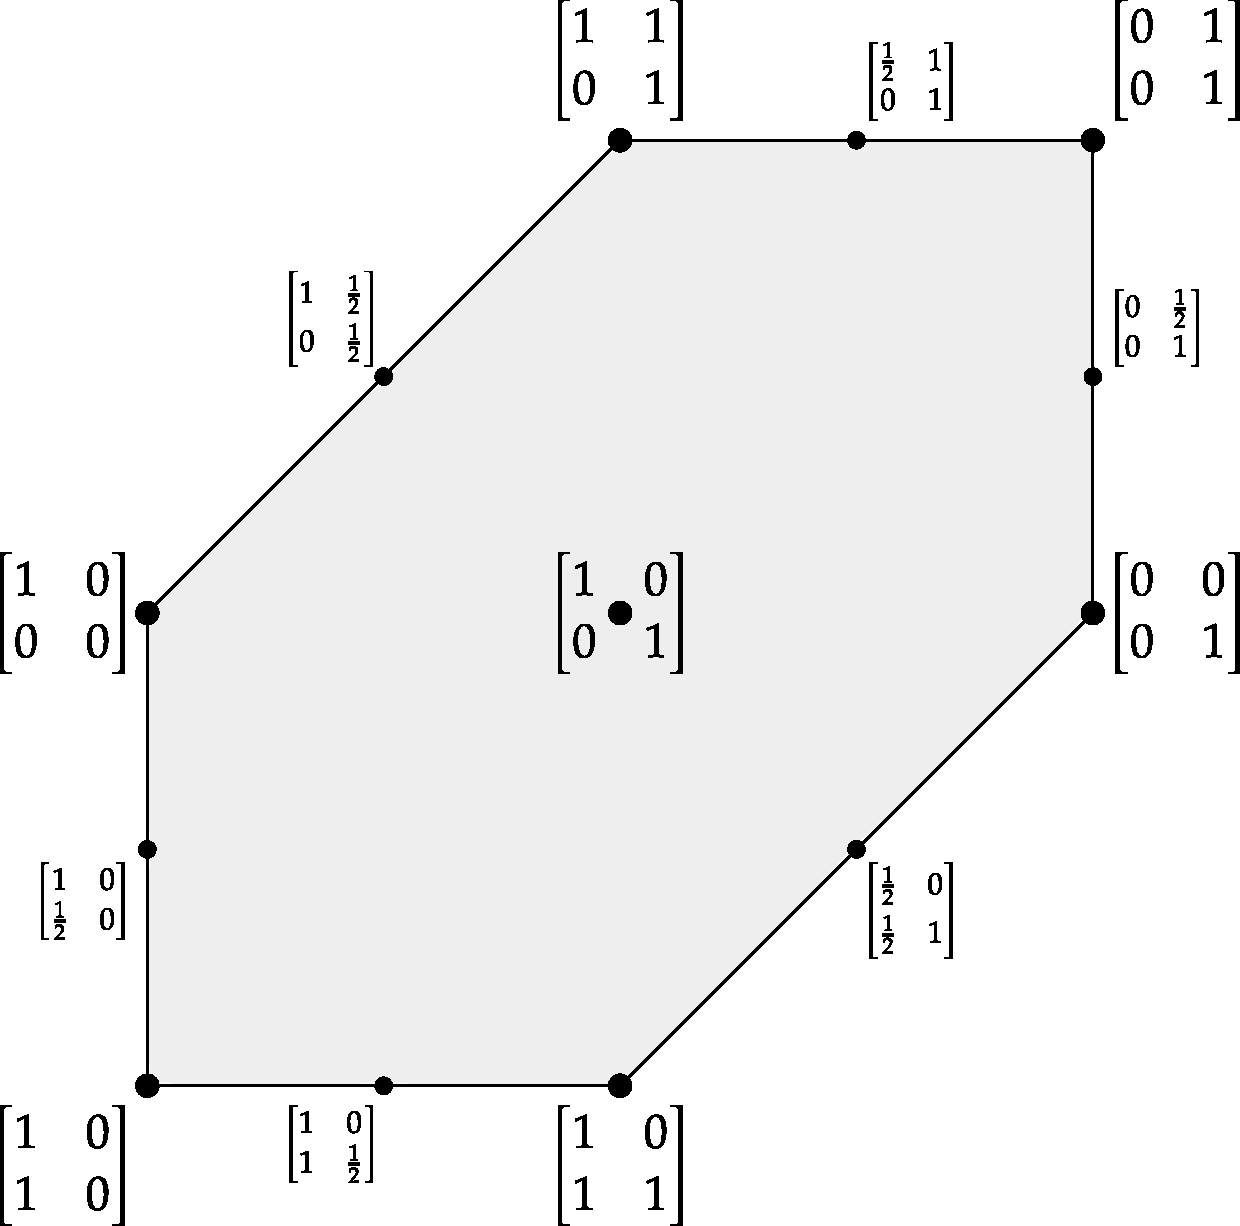
\includegraphics[width=0.65\linewidth]{space_UM2c.pdf}\\
  \caption{Space of utility matrices for binary classification.}
  \label{fig:space_UM}
\end{figure}
We can represent this space as in \fig~\ref{fig:space_UM}. The centre is the utility matrix with equal maximum utilities for correct classification and equal minimum utilities for incorrect classification; we shall see later that it corresponds to the use of accuracy as evaluation metric. Moving to the left from the centre, the utility for correct classification of class~1 decreases with respect of class~0; vice versa moving to the right. Moving upwards from the centre, the utility for misclassification of class~1 increases; moving downwards, the utility for misclassification of class~0 increases. We have excluded utility matrices in which misclassification has a higher utility than correct classification (although they may occur in some situations); they would appear in the missing the upper-left and lower-right corners. Fixing $(x,y)$ axes through the centre of the set, a utility matrix has coordinates
\begin{equation}
  \label{eq:coords_um}
  \begin{bmatrix}
    1 - x\ \delt(x > 0) & y\ \delt(y>0) \\
    -y\ \delt(y<0) & 1 + x\ \delt(x < 0)
  \end{bmatrix} \ .
\end{equation}

Note that this representation is \emph{not} meant to reflect any convex or metric properties, however. No metric or distance is defined in the space of utility matrices. Convex combination is defined if we drop the normalization~\eqref{eq:normalize_utilities} % and will be discussed in \sect~\mynotep{\ldots},
but it is not correctly reflected in the representation of \fig~\ref{fig:space_UM}.

\subsection{Relationship with common metrics}
\label{sec:common_metrics}

In \sect~\ref{sec:admissible_metrics} we found that the most general evaluation metric according to decision theory must be a linear combination of the confusion-matrix elements. The coefficients of this linear combination cannot depend on the confusion-matrix elements themselves, because such a dependence would reflect some sort of cognitive bias. Which common popular metrics adhere to this mathematical form? We want to answer this question in the binary-classification case and by giving as much allowance as possible in the typical context in which popular metrics are used.

Consider the case in which we are comparing several classifiers \emph{on the same test set}. The number of data $N$ and the relative frequencies $f_{0}, f_{1}$ with which the two classes \enquote{$0$}, \enquote{$1$} occur in the test set are fixed and constant for all classifiers under evaluation.

A classifier yields a normalized confusion matrix $(C_{ij})$ which we write in the format
\begin{equation*}
  \rotatebox[origin=c]{90}{
    \clap{\textit{\parbox{5em}{\centering\scriptsize classifier\\output\\$1\hspace{1.5em}0$}}
    }}\ 
    \overbracket[0pt]{
      \begin{bmatrix} C_{00} & C_{01} \\ C_{10} & C_{11}
      \end{bmatrix}}^{
      \clap{\textit{\parbox{6em}{\centering\scriptsize true class\\$0\hspace{3em}1$}}
    }} \ .
\end{equation*}

Owing to the constraints $C_{00} + C_{10} \equiv f_{0}$ and $C_{01} + C_{11} \equiv f_{1}$ we can always make two elements of the confusion matrix appear or disappear from any formula, replacing them with expressions involving the remaining two elements and the class frequencies. To avoid ambiguities in interpreting the functional form of mathematical formulae, let us agree to always express them in terms of $C_{00}$ and $C_{11}$ only, making the replacements $C_{10} = f_{0} - C_{00}$, $C_{01} = f_{1} - C_{11}$ wherever necessary.

Recall that given a utility matrix we can always modify its elements by a common positive multiplicative constant $a$ and by a common additive constant $b$, \eqn~\eqref{eq:modify_UM}, because such a modification corresponds to a change of unit and zero of the utility scale. With such a modification the evaluation metric~\eqref{eq:final_utility} takes the equivalent form
\begin{equation}
  \label{eq:final_utility_modified}
 a\ \sum_{ij} \ U_{ij}\ C_{ij} + b
\end{equation}
because $\sum_{ij} C_{ij} \equiv 1$. Writing the sum explicitly and rewriting the elements $C_{10}, C_{01}$ in terms of $C_{00}, C_{11}$ as discussed above, this formula becomes 
\begin{equation}
  \label{eq:final_utility_binary}
    a\ (U_{00} - U_{10})\ C_{00} \ + \ 
    a\ (U_{11} - U_{01})\ C_{11} \ + \ 
    a\ f_{0}\ U_{10} + a\ f_{1}\ U_{01} +  b \ .
\end{equation}

Since in the present context $N, f_{0}, f_{1}$ are constants, we are free to construct the arbitrary constants $a > 0$ and $b$ from them in any way we please:
\begin{equation}
  \label{eq:constants_functions}
  a = a(N, f_{0}, f_{1}) > 0\ , \qquad
  b = b(N, f_{0}, f_{1}) \ .
\end{equation}
We can also use this freedom to include the term $a\ f_{0}\ U_{10} + a\ f_{1}\ U_{01}$ into $b$ in the formula above. We conclude that \emph{an evaluation metric for binary classification complies with decision theory if and only if it can be written in the general form}
\begin{equation}
  \label{eq:general_valuation_metric}
  a(N, f_{0}, f_{1})\ \cx\ C_{00} +
  a(N, f_{0}, f_{1})\ \cy\  C_{11} +
  b(N, f_{0}, f_{1})
\end{equation}
\emph{where $\cx,\cy$ are constants that do not depend on $C_{00}, C_{11}, N, f_{0}, f_{1}$, and $a(\dotv)>0$, $b(\dotv)$ are arbitrary functions of $N, f_{0}, f_{1}$ only.}

A monotonic function (such as an exponential) of such form is also admissible, if we only require a comparison score to rank several classifiers from best to worst.

Let us examine some common evaluation metrics for binary classification from this point of view. We write their formulae in terms of $C_{00}, C_{11}$.

The following metrics are particular instances of formula~\eqref{eq:general_valuation_metric}:
\begin{itemize}
\item[\itemyes] \emph{Accuracy:} $C_{00}+C_{11}$. We have $a=1$, $\cx=\cy=1$, $b=0$. Indeed it corresponds to the utility yield based on the identity utility matrix $(U_{ij}) = \begin{bsmallmatrix} 1&0\\0&1 \end{bsmallmatrix}$ (or equivalently a utility matrix that assigns the same utility to the correct classification of any class, and the same, lower utility to the misclassification of any class).
  
\item[\itemyes] \emph{True-positive rate (recall):} $C_{00}/f_{0}$. Here $a=1/f_{0}$, $\cx=1$, $\cy=0$, $b=0$. It corresponds to using the utility matrix $\begin{bsmallmatrix} 1&0\\0&0 \end{bsmallmatrix}$. 

\item[\itemyes] \emph{True-negative rate (specificity):} $C_{11}/f_{1}$. Here $a=1/f_{1}$, $\cx=0$, $\cy=1$, $b=0$. It corresponds to using the utility matrix $\begin{bsmallmatrix} 0&0\\0&1 \end{bsmallmatrix}$. 
\end{itemize}

The following metrics instead \emph{cannot} be written in the form~\eqref{eq:general_valuation_metric}, nor as monotonic functions of that form:
\begin{itemize}
\item[\itemno] \emph{Precision:} $C_{00}/(C_{00}-C_{11}+f_{1})$. Non-linear in $C_{00}, C_{11}$.

\item[\itemno] \emph{$F_{1}$-measure:} $2 C_{00}/(C_{00} - C_{11} + 1)$. Non-linear in $C_{00}, C_{11}$. The same is true for the more general $F_{\beta}$-measures.

\item[\itemno] \emph{Matthews correlation coefficient:} $\frac{
    f_{1}\,C_{00} + f_{0}\,C_{11}}{\sqrt{
      f_{0}\ f_{1}\ (f_{1} + C_{00} - C_{11})\ (f_{0} + C_{11} - C_{00})
    }}$. Non-linear in $C_{00}, C_{11}$.

\item[\itemno] \emph{Fowlkes-Mallows index:} $C_{00}/\sqrt{
      f_{0}\ (f_{1} + C_{00} - C_{11})}$. Non-linear in $C_{00}, C_{11}$.

  \item[\itemno] \emph{Balanced accuracy:} $C_{00}/(2 f_{0}) + C_{11}/(2 f_{1})$. Despite being linear in $C_{00}, C_{11}$ and an average of two metrics (true-positive and true-negative rate) that are instances of formula~\eqref{eq:general_valuation_metric}, it is not an instance of that formula, because the two averaged metrics involve different $a(\dotv)$ functions.
\end{itemize}

We see that many popular evaluation metrics do not comply with the principles of decision theory. Any such metric suffers from two problems.

First, as discussed in \sect~\ref{sec:decision_theory} the metric involves an interdependence of utilities and classification frequencies, which implies some form of cognitive bias\autocites[discuss such biases in regard to the $F_{1}$-measure]{handetal2018}.

Second, the ranking of confusion matrices yielded by the metric does not fully agree with that yielded by any utility matrix -- a full agreement would otherwise imply that the metric could be written in the form~\eqref{eq:general_valuation_metric}. Some confusion matrices must therefore be incorrectly ranked. Since any rational classification problem is characterized by some underlying utility matrix, this means that the incompliant metric will always lead to some wrong evaluations. By contrast, compliant metrics such as the accuracy give completely correct rankings for all pairs of confusion matrices at least in a specific set of classification problems.

The second phenomenon is illustrated in the plots of \figs~\ref{fig:metrics_vs_utility}--\ref{fig:metrics_vs_utility2}.
% \setlength{\fboxsep}{0pt}%
% \setlength{\fboxrule}{0.25pt}%
\begin{figure}[p]
  \centering
  % {A}\hfill\mbox{}\\[0pt]
%  \vspace{-0.5\headsep}
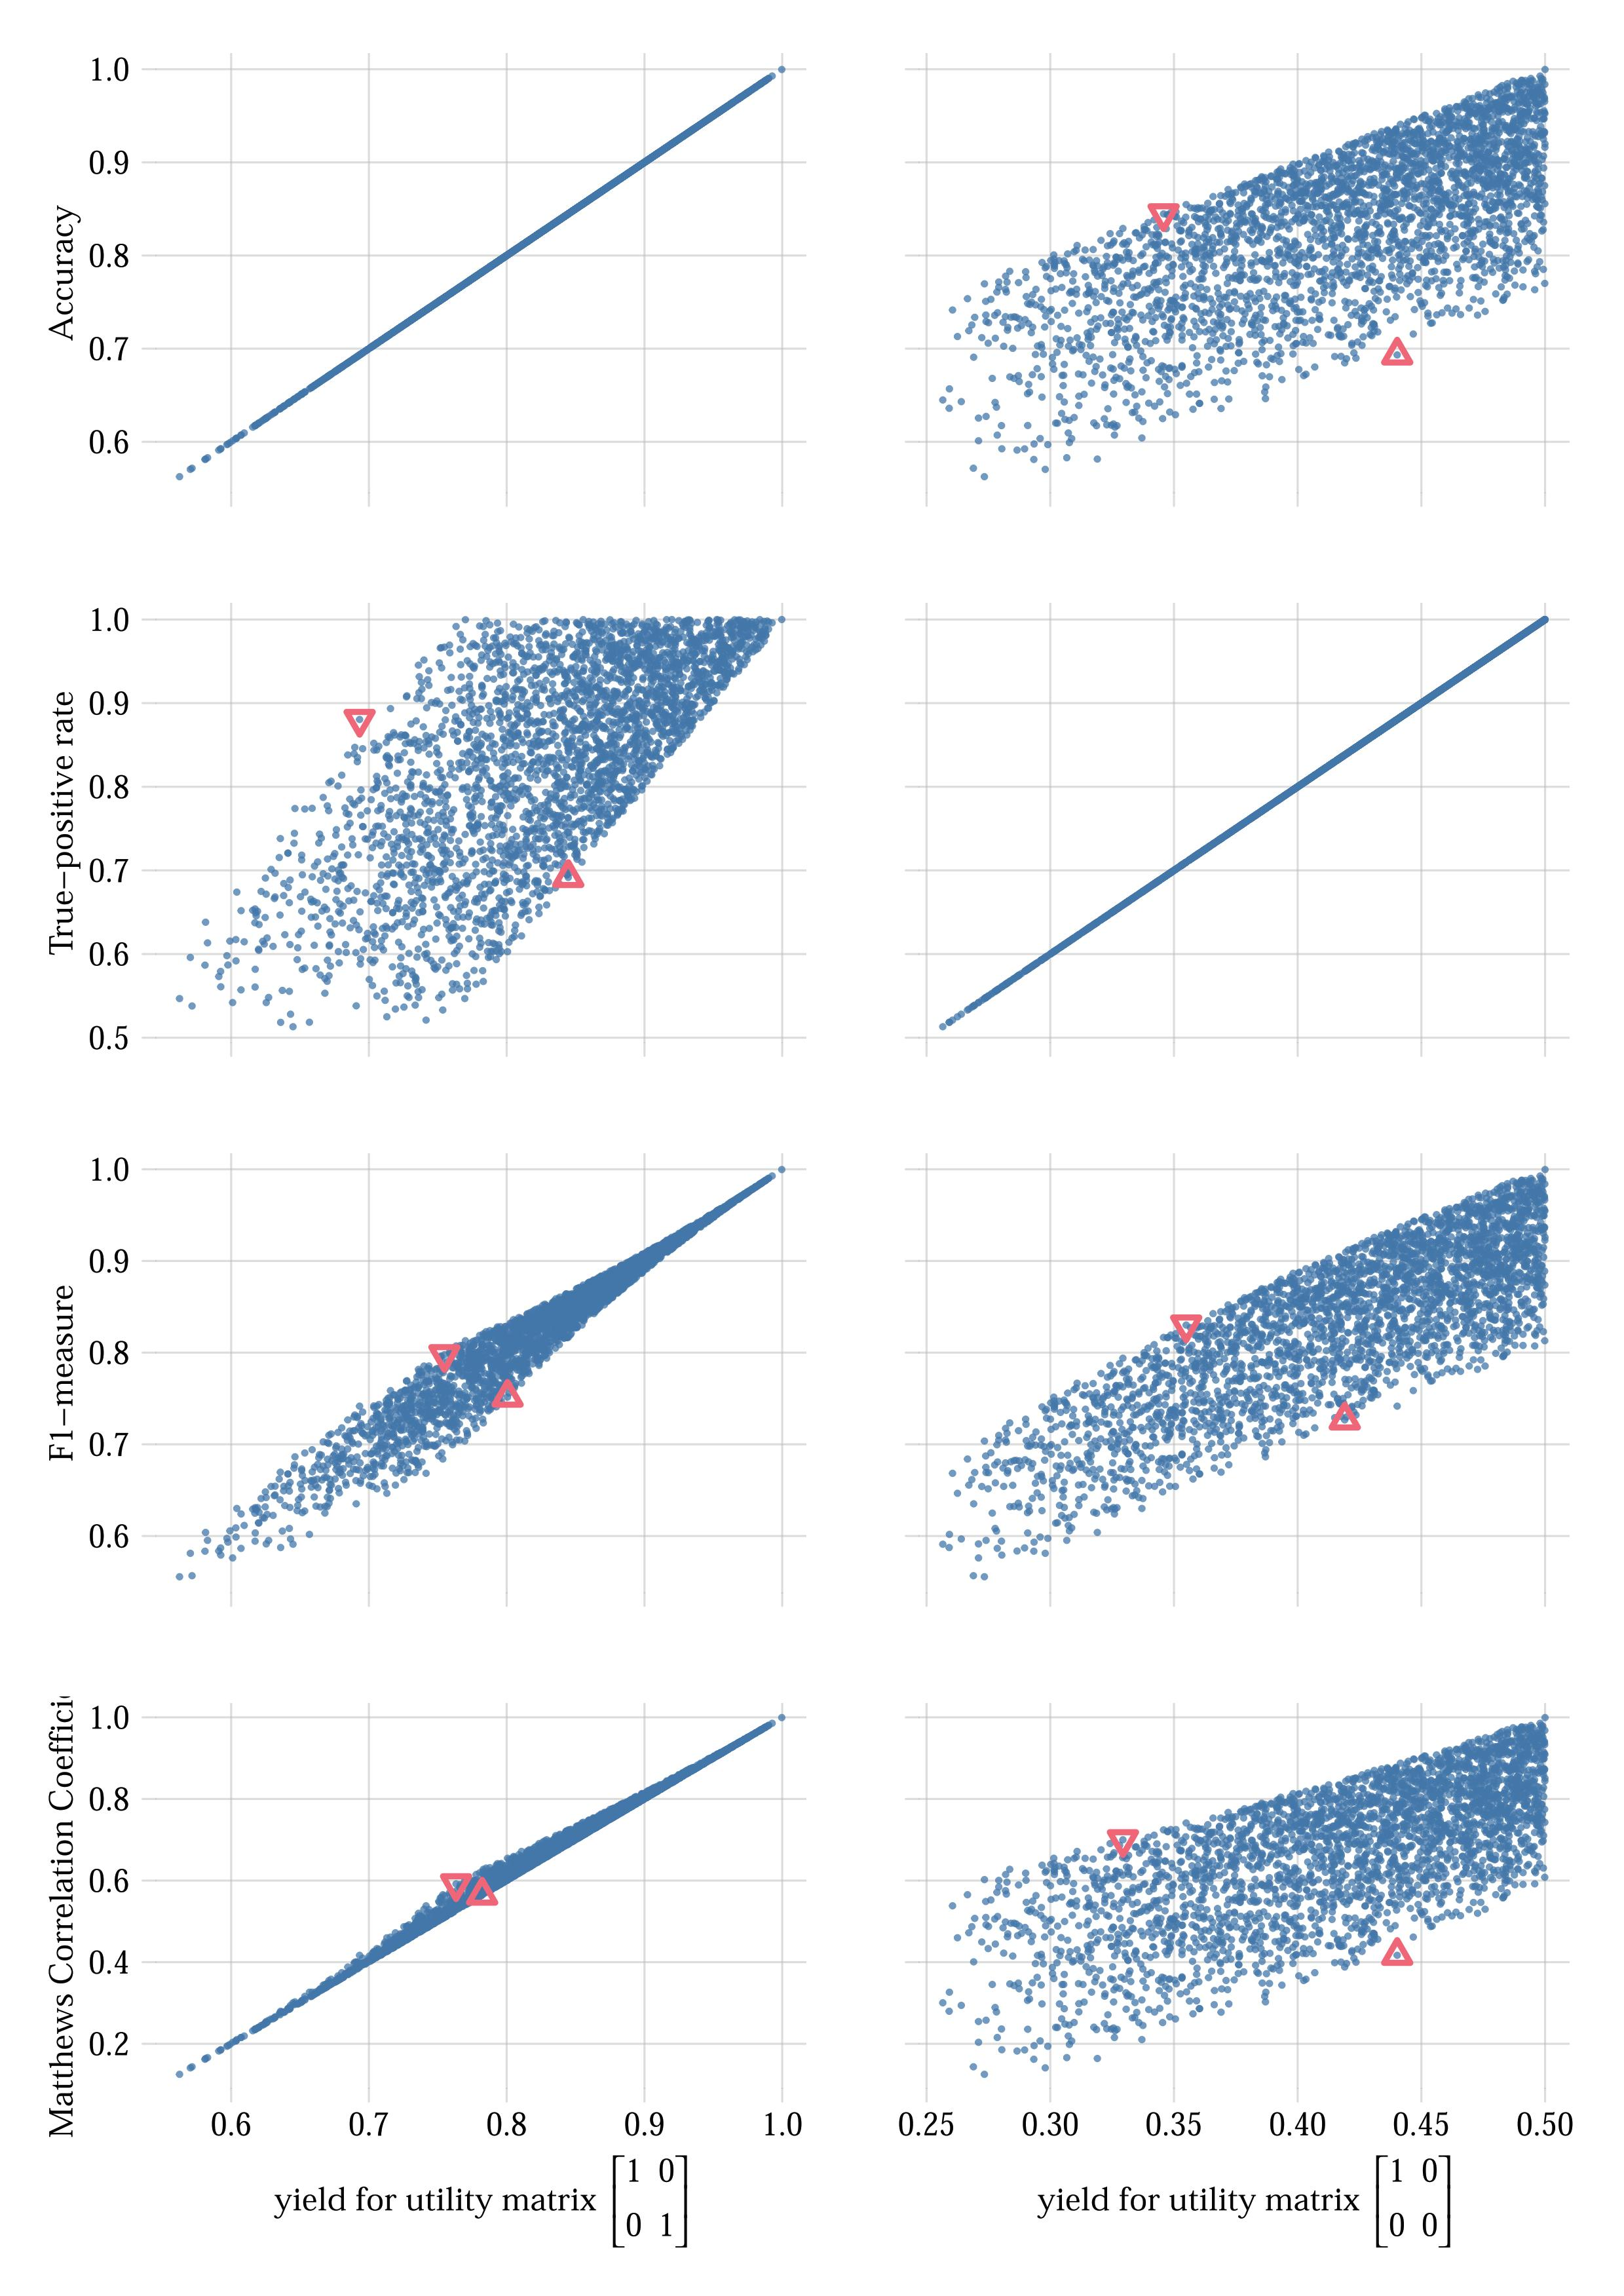
\includegraphics[width=0.95\linewidth]{utility_vs_metrics2_0.5.jpg}\\%[-1\baselineskip]
% {B}\hfill\mbox{}\\[0pt]
% \vspace{-1em}{\color{mygrey}\rule{0.66\linewidth}{0.25pt}}
% 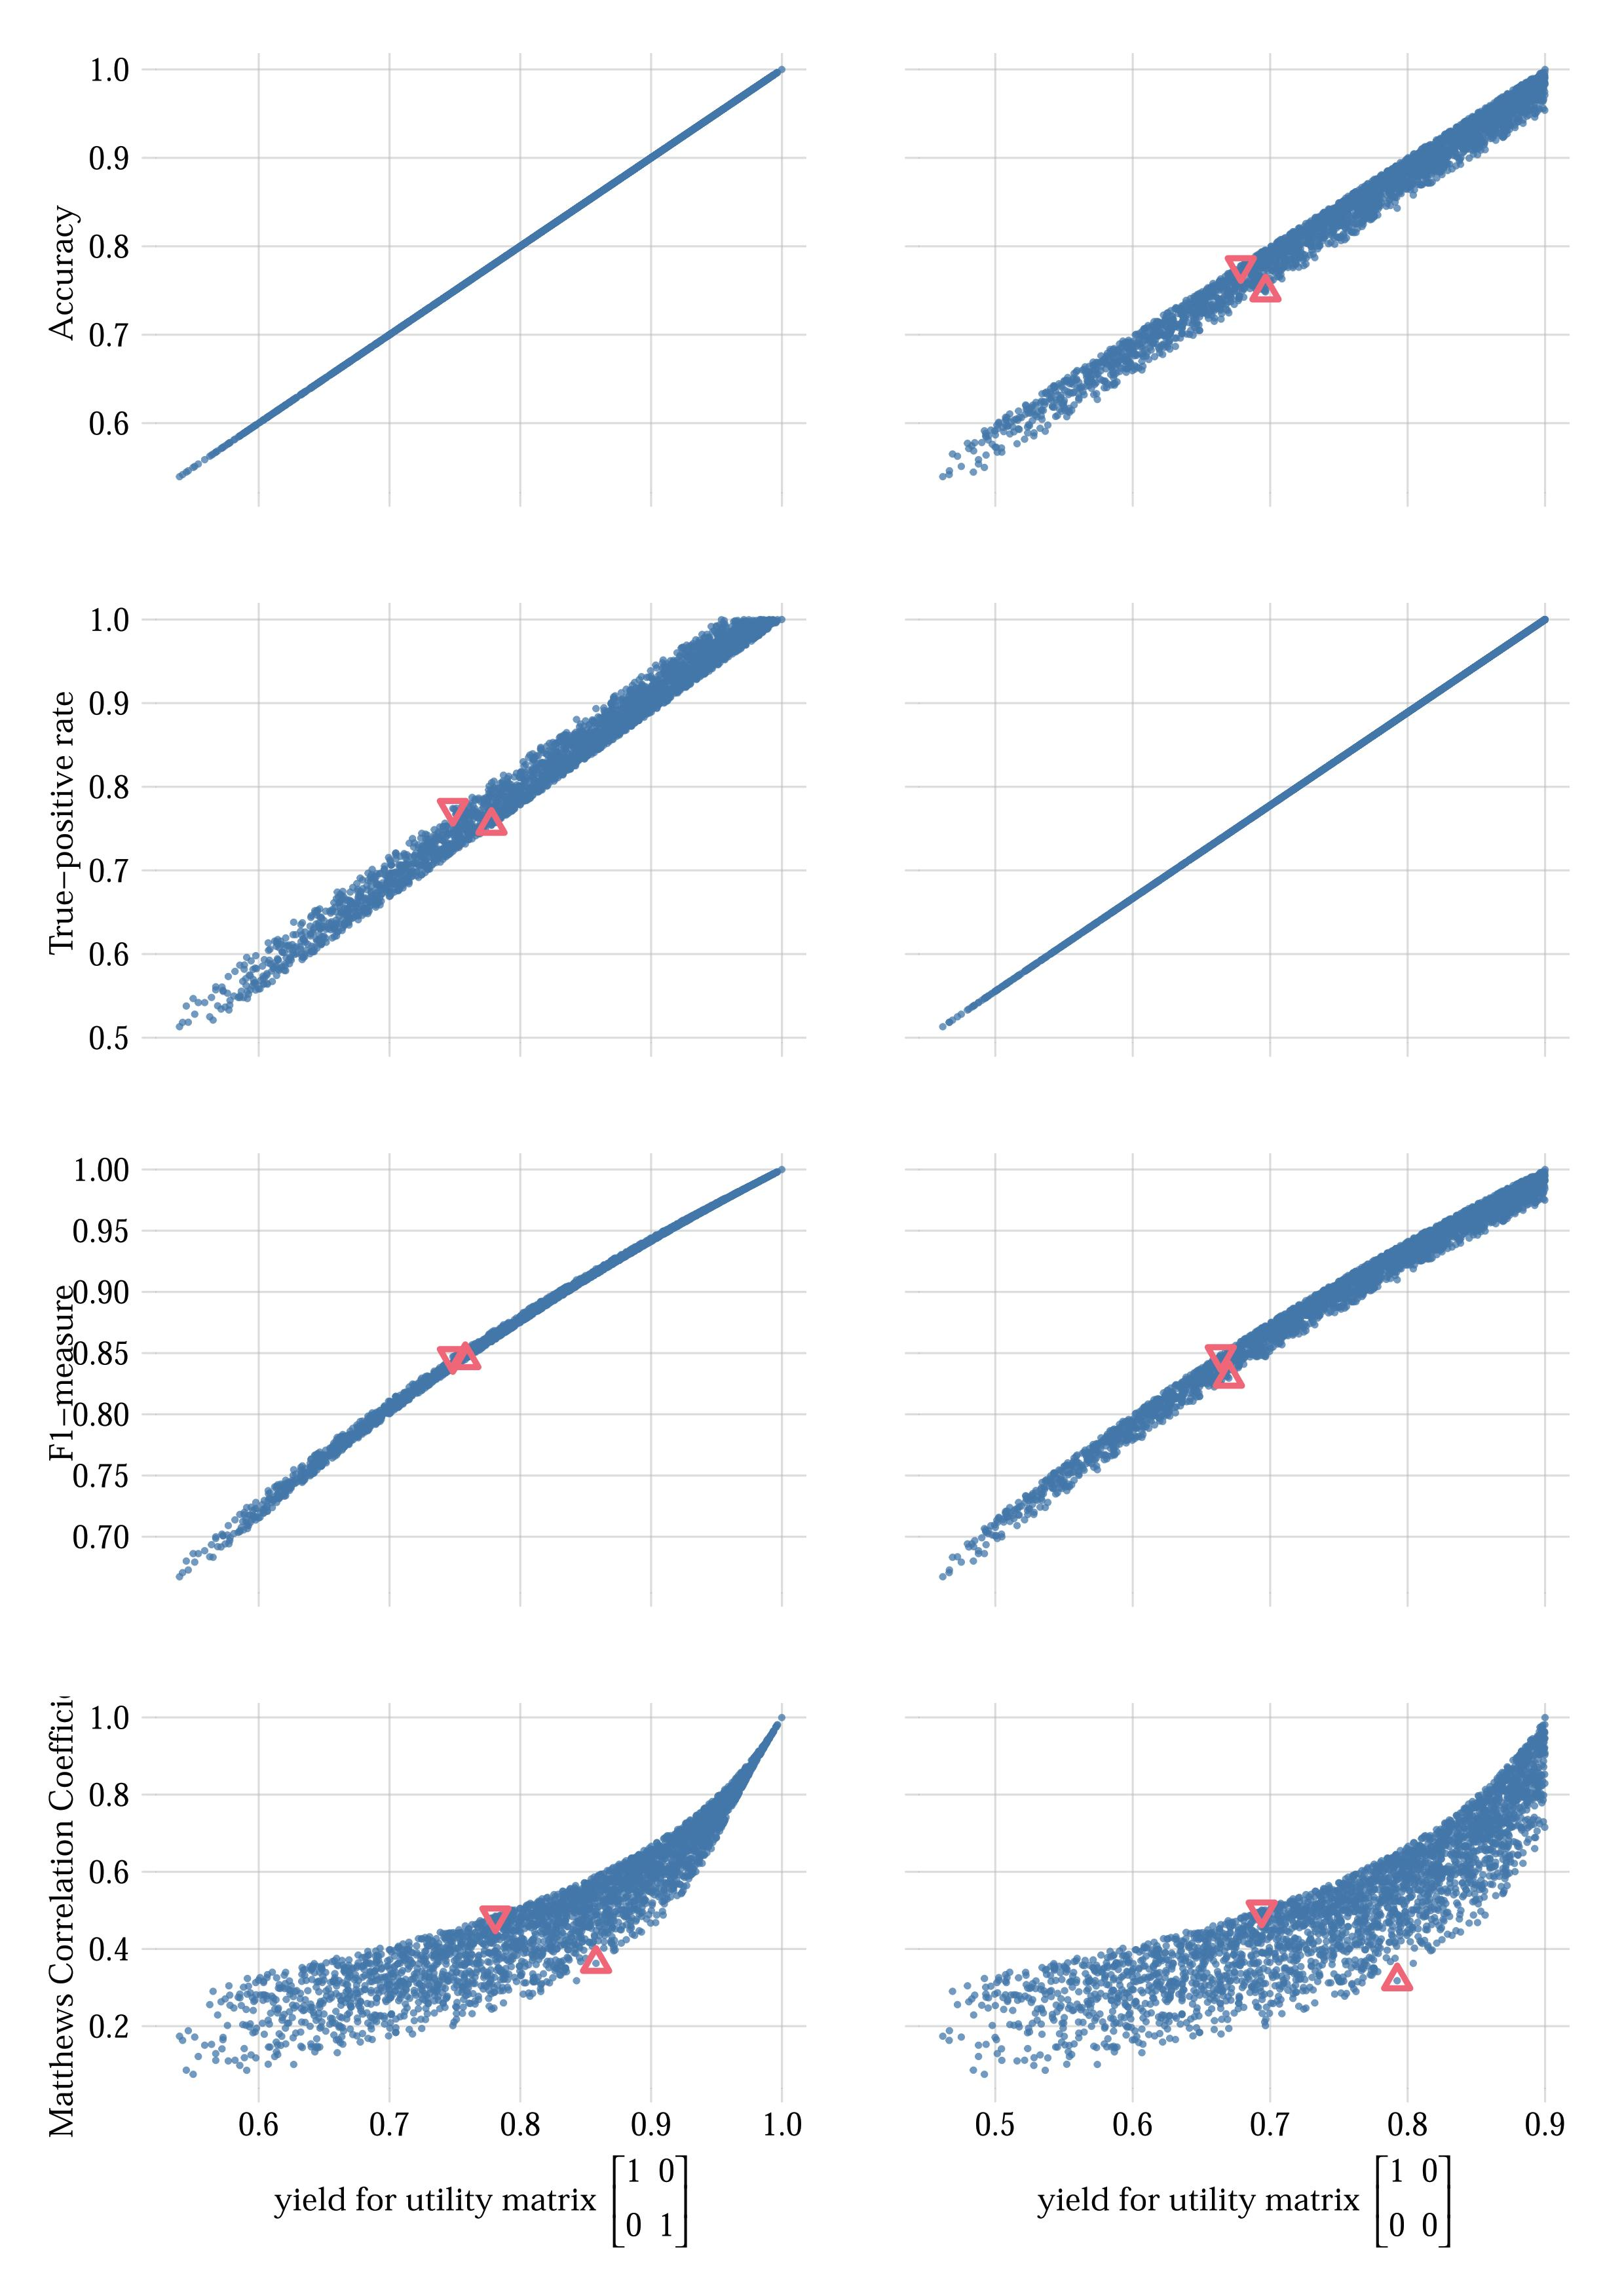
\includegraphics[width=0.95\linewidth]{utility_vs_metrics2_0.9.jpg}\\[0pt]
\caption{Relationship between various evaluation metrics and actual utility yields for a  two binary-classification problems with underlying utility matrices $\begin{bsmallmatrix} 1&0\\0&1 \end{bsmallmatrix}$ (left column) and $\begin{bsmallmatrix} 1&0\\0&0 \end{bsmallmatrix}$ (right column). All confusion matrices ({\color{mypurpleblue}blue dots}) are obtained from a dataset with 50\%/50\% class balance.
%
  Pairs of {\color{myred}red triangles} in a plot show two confusion matrices which are wrongly ranked by the metric (y-axis) with respect to the actual utility yield (x-axis). Clearly there can even be three or more confusion matrices ranked in completely reverse order by the metric.
%
  % {\color{myred}Red triangular pairs} (almost overlapping in some plots) in each column show two confusion matrices wrongly ranked by \emph{all} metrics but one simultaneously.
  %%
  The accuracy yields correct evaluations the classification problem on the left column; and the true-positive rate, for the one on the right. }
  \label{fig:metrics_vs_utility}
\end{figure}
%%
\begin{figure}[p]
  \centering
  %{A}\hfill\mbox{}\\[0pt]
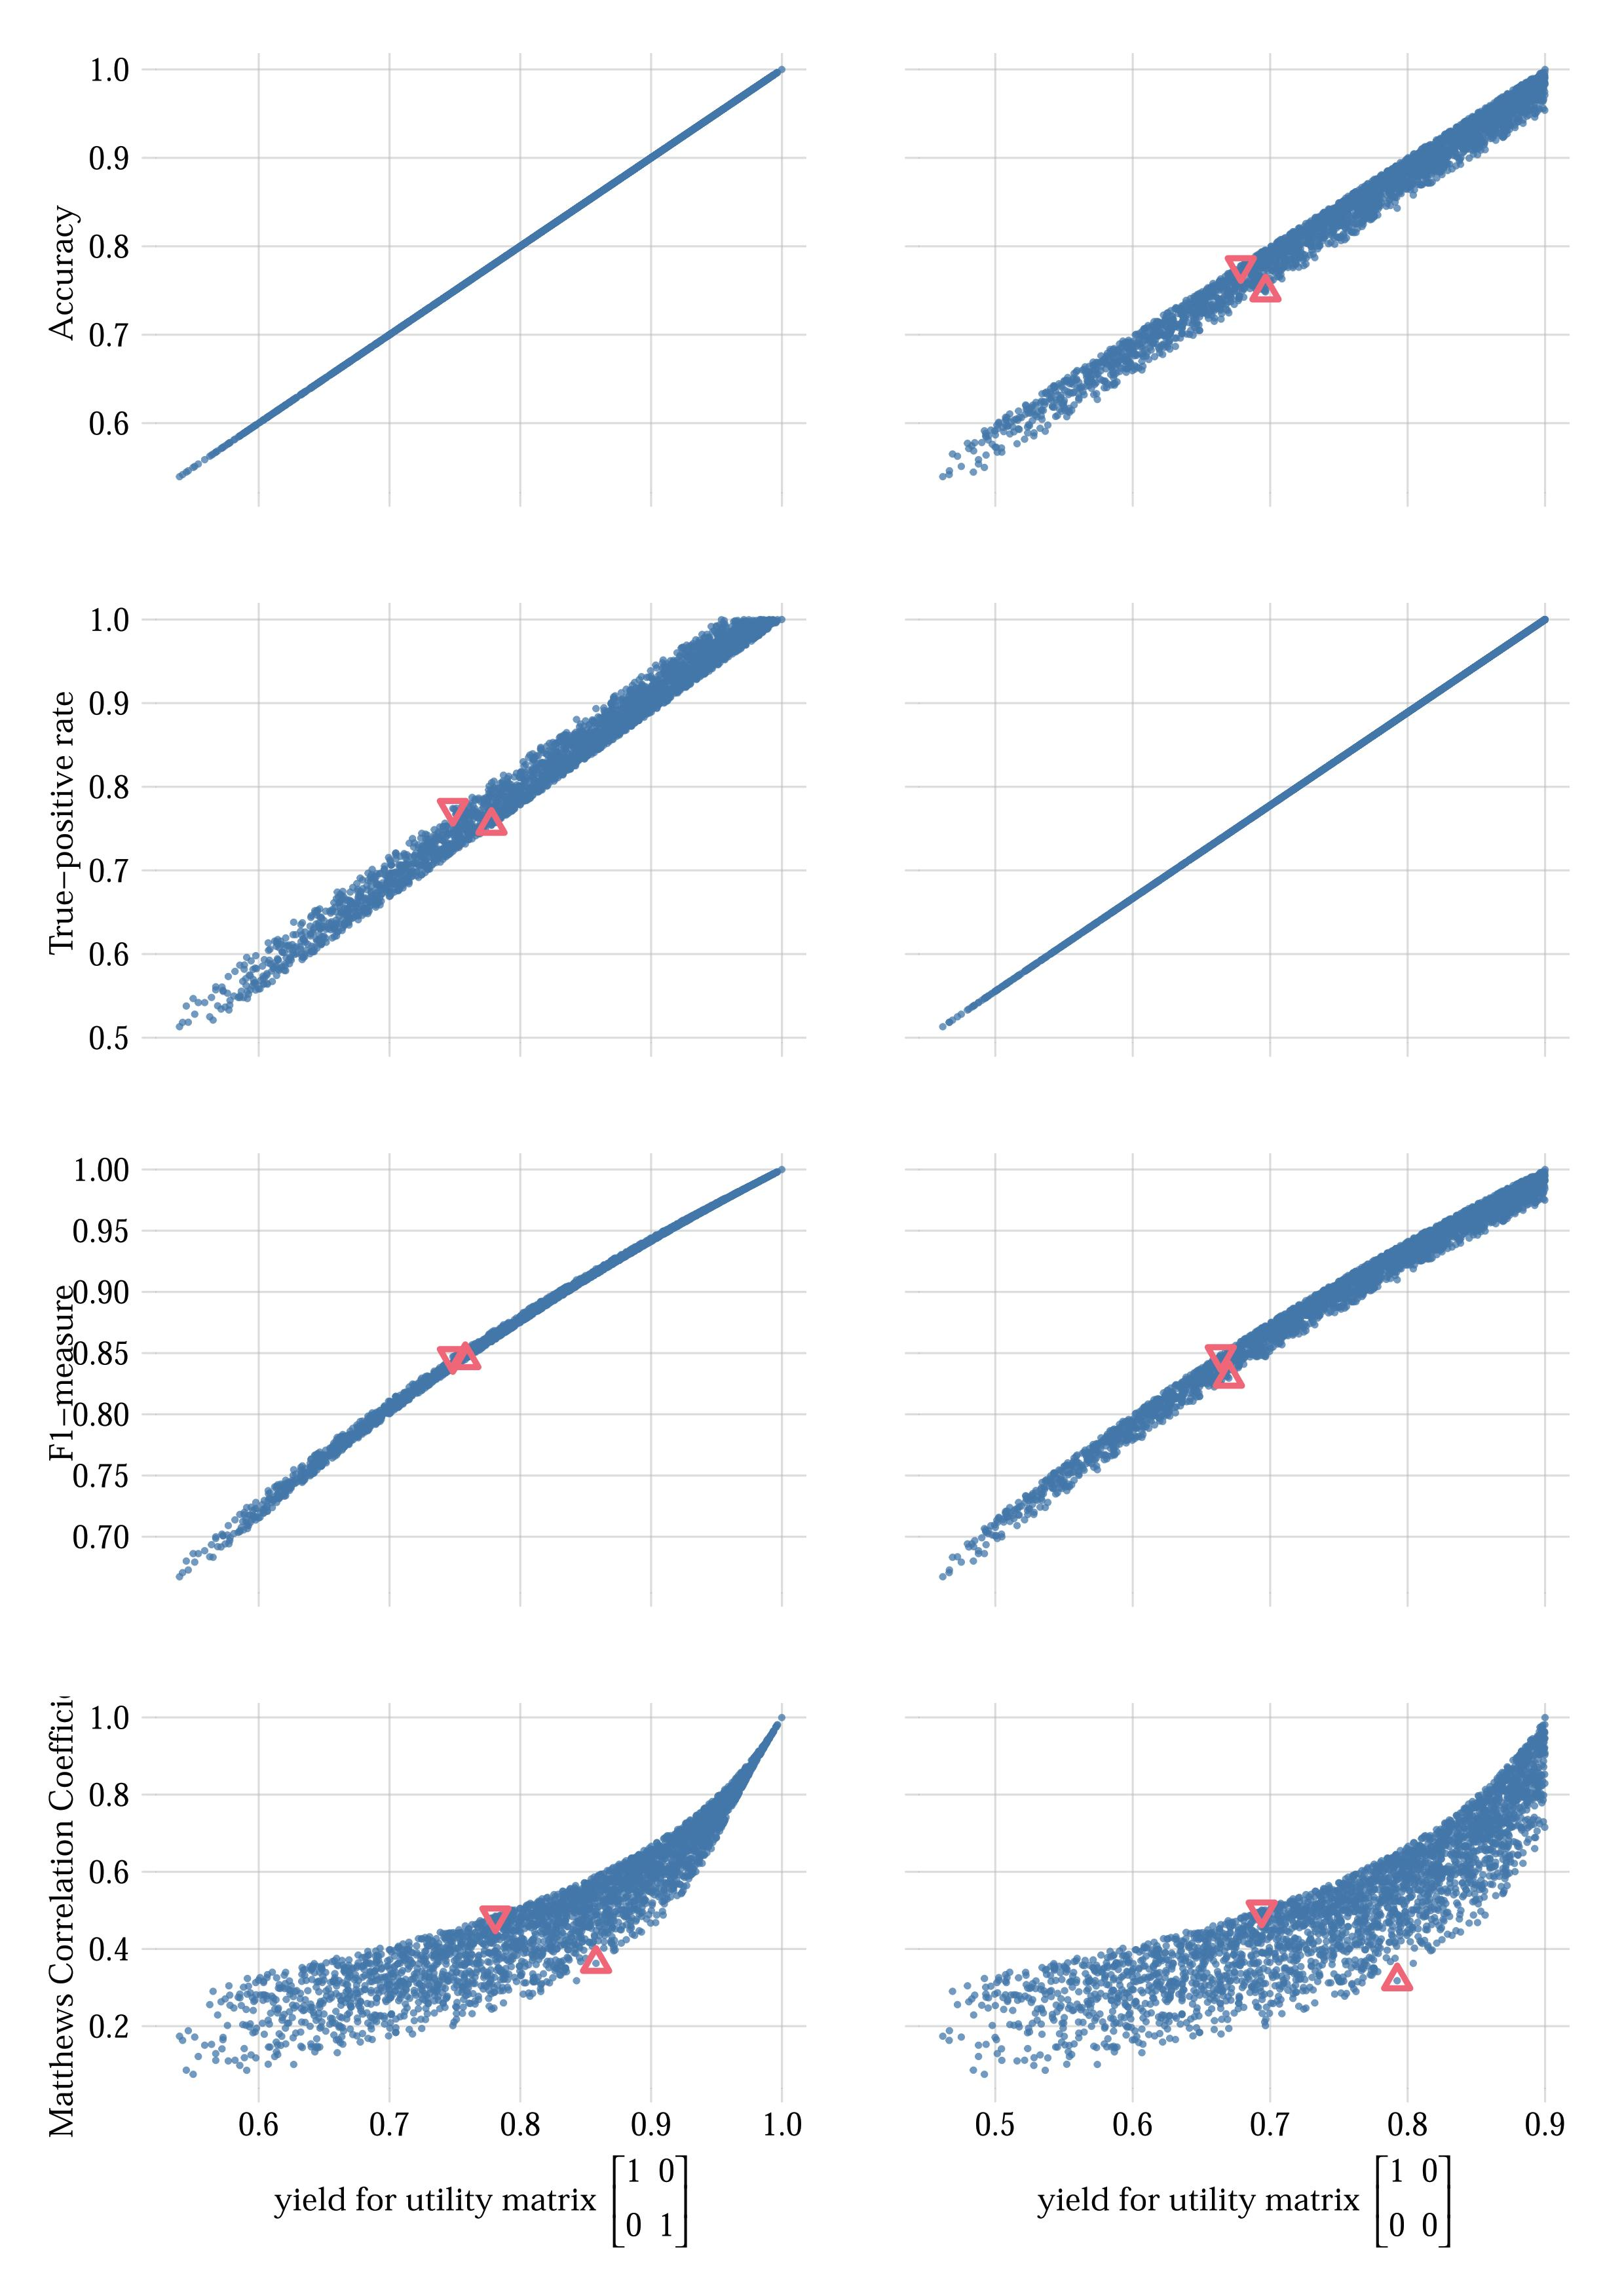
\includegraphics[width=0.95\linewidth]{utility_vs_metrics2_0.9.jpg}\\%[0pt]
% {B}\hfill\mbox{}\\[0pt]
% \vspace{-1em}{\color{mygrey}\rule{0.66\linewidth}{0.25pt}}
% 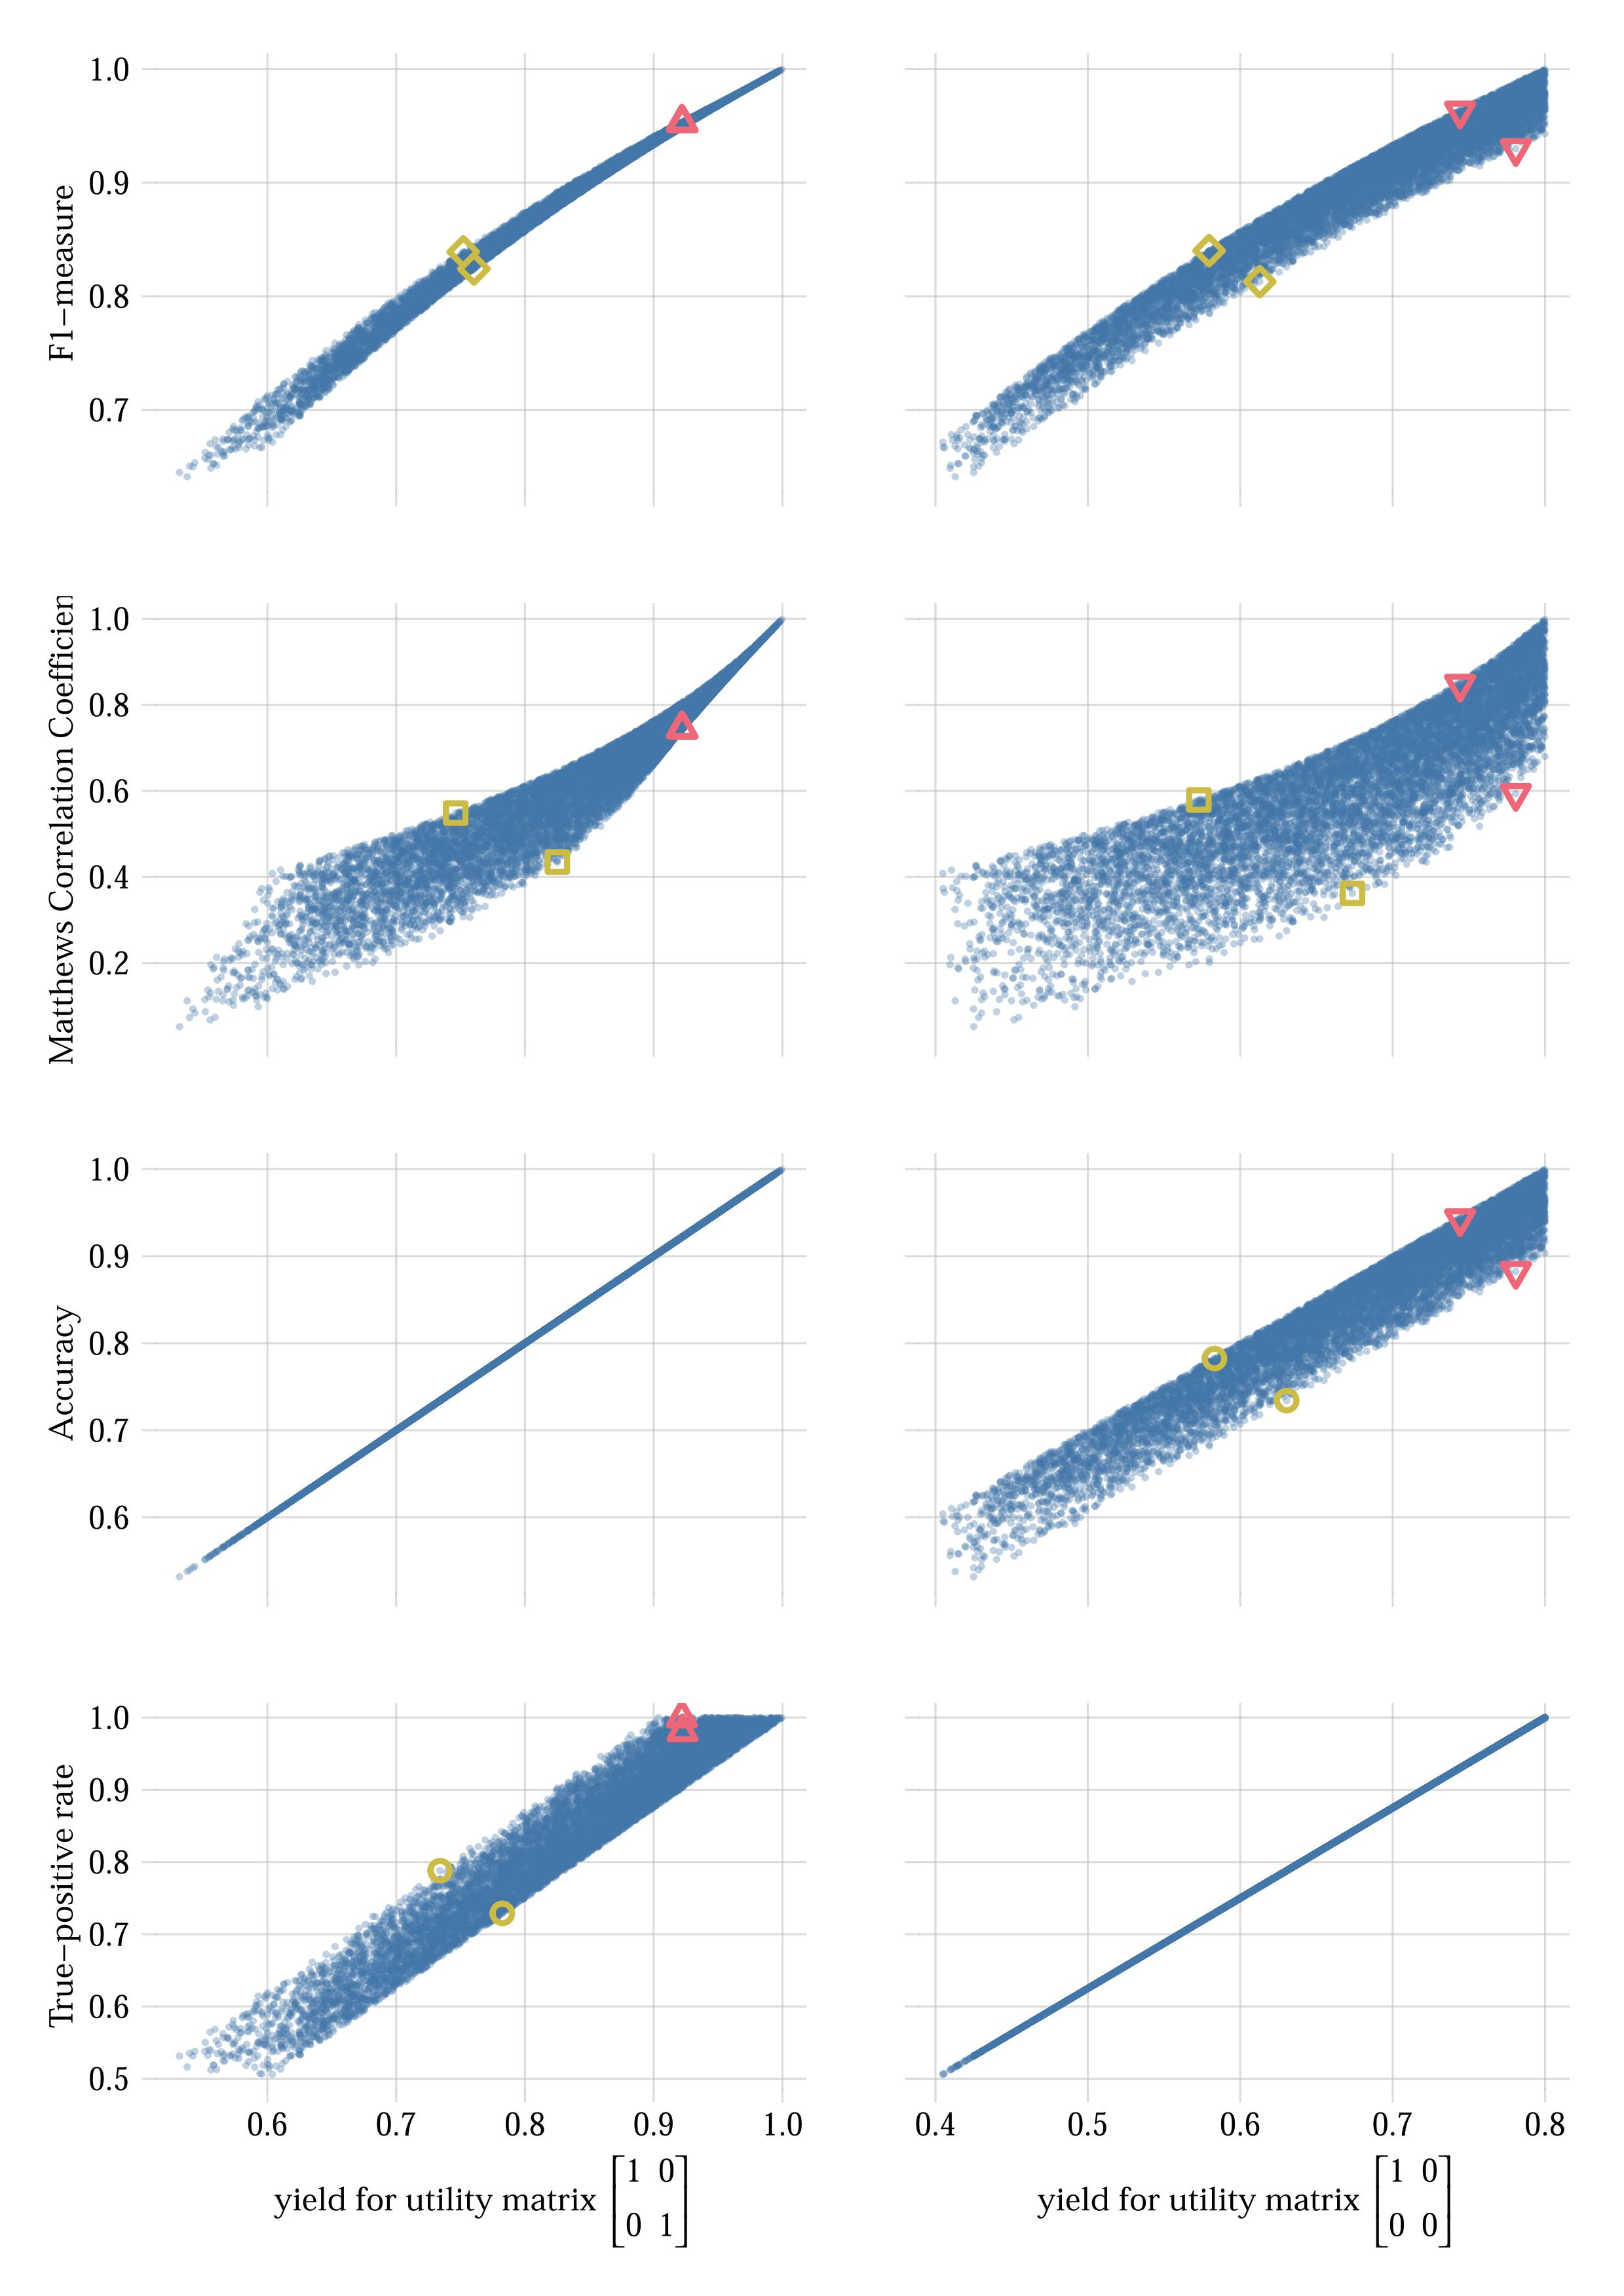
\includegraphics[width=0.99\linewidth]{utility_vs_metrics_0.8.jpg}\\
\caption{As for \fig~\ref{fig:metrics_vs_utility} but for confusion matrices obtained from an imbalanced dataset with 90\% occurrence of class~0 (\enquote{positive}) and 10\% of class~1 (\enquote{negative}).}
  \label{fig:metrics_vs_utility2}
\end{figure}
Each blue dot in a plot represents a hypothetical confusion matrix obtained from a test dataset in a binary-classification problem. The dot's coordinates are the utility yield of that confusion matrix according to a particular utility matrix underlying the classification problem, and the score of the confusion matrix according to another metric. The underlying utility matrix is $\begin{bsmallmatrix} 1&0\\0&1 \end{bsmallmatrix}$ for all plots in the left column, and $\begin{bsmallmatrix} 1&0\\0&0 \end{bsmallmatrix}$ for all plots in the right column. The other metrics considered, one for each row of plots, are accuracy, true-positive rate (recall, class~0 being \enquote{positive}), $F_{1}$-measure, Matthews correlation coefficient.

The confusion matrices are selected by first fixing a proportion of classes in the dataset, which is 50\%/50\% (balanced dataset) for all plots in \fig~\ref{fig:metrics_vs_utility} and 90\%/10\% (imbalanced dataset) for all plots in \fig~\ref{fig:metrics_vs_utility2}; and then choosing true-positive and true-negative rates independently distributed between $1/2$ and $1$ with linearly increasing probabilities. These confusion matrices therefore represent the classification statistics produced %(one and the same in each figure)
by classifiers that tend to have good performance -- as is clear from the fact that the points tend to accumulate on the upper-right corners of the plots.

% Consider the uppermost left plot of \fig~\ref{fig:metrics_vs_utility} as an example. It corresponds to a binary-classification problem with an underlying utility matrix equivalent to the identity $ \begin{bsmallmatrix} 1&0\\0&1 \end{bsmallmatrix} $, and a test set with a balanced number of classes, that is, each class appear with $50\%$ frequency. We select a large number of confusion matrices having this class balance and true-positive and true-negative rates distributed between $1/2$ and $1$ with linearly increasing probabilities. These confusion matrices would thus arise mostly from good classifying algorithms. For each confusion matrix we calculate
% \begin{enumerate}[label=\arabic*.]
% \item its average utility yield, according to the utility matrix $\begin{bsmallmatrix} 1&0\\0&1 \end{bsmallmatrix}$; this number is the actual performance, appropriate to this specific problem, of the corresponding algorithm;
% \item its score according to another metric, in this case the $F_{1}$-measure;
% \end{enumerate}
% and we plot (blue disks) a corresponding point with these two numbers as $x$- and $y$-coordinates. This plot thus shows the general statistical relation between the appropriate utility score and the $F_{1}$-measure of this distribution of confusion matrices.
% 
% The other three plots in the upper panel of \fig~\ref{fig:metrics_vs_utility} are analogous but for Matthews Correlation Coefficient, accuracy, and true-positive rate as $y$-coordinates. The lower panel is analogous to the upper panel, but for an imbalanced dataset with one class appearing with $80\%$ frequency. Finally, \fig~\ref{fig:metrics_vs_utility2} is analogous to \fig~\ref{fig:metrics_vs_utility} but with an underlying utility matrix equal to $ \begin{bsmallmatrix} 1&0\\0&0 \end{bsmallmatrix} $.

We see that the accuracy (first-row plots) always gives correct relative evaluations of all confusion matrices when the underlying utility matrix is equivalent to $\begin{bsmallmatrix} 1&0\\0&1 \end{bsmallmatrix}$ (left column): the y-coordinate is a monotonically increasing function -- in fact a linear function -- of the x-coordinate. Accuracy is indeed the utility yield corresponding to the identity utility matrix. The true-positive rate (second-row plots) always gives correct relative evaluations (provided the test set is the same) when the underlying utility matrix is equivalent to $\begin{bsmallmatrix} 1&0\\0&0 \end{bsmallmatrix}$ (right column). When each of these two metrics is used for a problem having different underlying utility matrix, however, there is no deterministic relationship between the metric's score and the actual utility yield: the y-coordinate is not a function of the x-coordinate. Thus it is always possible to find two or more confusion matrices for which the metric gives completely reversed evaluations with respect to the actual utility yield, scoring the worst confusion matrix -- and thus its associated algorithm -- as the best, and the best as the worst. Pairs of red triangular shapes in a plot are examples of confusion matrices wrongly ranked by the y-axis metric.

Metrics such as accuracy and true-positive rate, complying with formula~\eqref{eq:general_valuation_metric}, thus require us to rely on evaluation \emph{luck} only when they are used in the wrong classification problem.

The plots for the $F_{1}$-measure (third-row plots) and Matthews correlation coefficient (fourth-row plots) show that these two metrics do not have any functional relationship with the actual utility yield. It is again always possible to find two or more confusion matrices for which either metric gives completely reversed evaluations with respect to the actual utility yield. But for these two metrics, unlike accuracy and true-positive rate, cases of incorrect evaluation will \emph{always} occur, in every classification problem.

Metrics such as  $F_{1}$-measure and Matthews correlation coefficient, not complying with formula~\eqref{eq:general_valuation_metric}, thus \emph{always require us to rely on luck in our evaluations}. There are no classification problems for which these metrics lead to always correct evaluations.

\medskip

A metric non-compliant with decision theory can lead to a large number of correct results for some classification problems and test sets. The bottom-left plot of \fig~\ref{fig:metrics_vs_utility}, for instance, shows that the Matthews correlation coefficient is almost a monotonically increasing deterministic function of the utility yield when the underlying utility matrix is the identity and the dataset is balanced (but it is not when the underlying utility matrix is $\begin{bsmallmatrix} 1&0\\0&0 \end{bsmallmatrix}$ or the dataset is imbalanced; see corresponding plots). Such an occasional partial agreement is useless, however. Knowledge of the utility matrix is a prerequisite for relying on such partial agreement-- but with this knowledge we can directly use the actual utility yield instead, which has an exact agreement and is easier to compute.


\section{Unknown or incorrect utilities}
\label{sec:unknown_wrong_utilities}

So far we have argued that the natural evaluation metric for a classifier is the utility yield of its confusion matrix, according to the utilities underlying the particular classification problem. We have also argued that many popular metrics, those not complying with formula~\eqref{eq:general_valuation_metric}, must lead to instances of incorrect evaluation. Our arguments are based on the principles of decision theory.

Several interrelated questions arise from our arguments, though:
\begin{itemize}
\item What to do when we are uncertain about the utilities underlying a classification problem?
\item What happens if the utilities we use are actually wrong, that is, not the true ones underlying the problem?
\item How often do uncompliant metrics such as $F_{1}$-measure or Matthews correlation coefficient lead to incorrect results, on average?
\end{itemize}
In fact, if a small error in the assessment of the utilities led to a large number of wrong evaluations, and at the same time incompliant metrics led a small number of wrong evaluations on average, then all the rigorousness of decision-theoretic metrics would be useless in practice, and  incompliant metrics would be best for real applications.

This is not the case, however. We now discuss how to deal with uncertainty about the utilities, and present an important result: Using wrong utilities, even with relative errors almost as large as 20\% of the maximum utility, still leads to fewer incorrect relative evaluations on average than using some of the most common metrics.

\subsection{Unknown utilities; average performance on several classification problems}
\label{sec:unknown_utilities}

Dealing with unknown utilities is straightforward. Suppose we are uncertain whether the utility matrix appropriate to a classification problem is $\uncu{1} \equiv \bigl(U^{(1)}_{ij}\bigr)$, or $\uncu{2}$, or $\uncu{3}$, and so on, where the number of alternatives can even be infinite or continuous. Each alternative $\uncu{a}$ has a probability $q_a$, or probability density $q(a)\ \di a$ in the continuous case. Then \emph{for the classification problem we should use the expected utility matrix
  \begin{equation}
    \label{eq:expe_UM}
    \aveu \defd q_{1}\ \uncu{1} + q_{2}\ \uncu{2} + q_{3}\ \uncu{3} + \dotsb
  \end{equation}
  or $\aveu \defd \int q(a)\, \uncu{a}\, \di a$ in the continuous case}.

We only give a sketch of the proof of this intuitive result. If we are uncertain about the utility matrix then we have a double decision problem: choosing the optimal utility and choosing the optimal class. If the true utility matrix is for instance $\uncu{2} \equiv \bigl(U^{(2)}_{ij}\bigr)$, and the true class is class~$0$, then choosing class~$1$ would yield a utility $U^{(2)}_{10}$; choosing class~$0$ would yield a utility $U^{(2)}_{00}$, and so on. Our double decision problem is thus characterized by a rectangular utility matrix that is the row-concatenation of the utility matrices $\uncu{a}$. We make the realistic judgement that the probabilities $q_{a}$ of the utility matrices and the probabilities $p_{j}$ of the classes are independent, so that $q_{a}\cdot p_{j}$ is probability that the true utility matrix is $\uncu{a}$ and the true class is $j$. The principle of maximum expected utility, \sect~\ref{sec:dt_utilities} \eqn~\eqref{eq:max_expe_utility}, then leads to the maximization of the expected utilities
\begin{equation}
  \label{eq:average_expe_utility}
  \eu_{i} \defd \sum_{j,a} U^{(a)}_{ij}\ q_{a}\cdot p_{j}
  \equiv \sum_{j} \biggl[\underbrace{\sum_{a} q_{a}\ U^{(a)}_{ij}}_{\aveu} \biggr]\ p_{j}
\end{equation}
in which the expected utility matrix~\eqref{eq:expe_UM} appears as the \enquote{effective} utility matrix to be used for the class-decision problem alone.

If our uncertainty is symmetric with respect to the utilities conditional on the different classes -- for instance, our uncertainty about the utilities conditional on class~$0$ is the same as on class~$1$ -- then the expected utility matrix is equivalent to the identity matrix. The utility yield is in this case equal to the accuracy. The accuracy is therefore the natural evaluation metric to use if we are in a complete state of uncertainty regarding the underlying utilities. This fact is indeed reflected in some results discussed in \sect~\ref{sec:wrong_utility_assess}.


For a binary-classification problem the set of possible utility matrices can be represented as in \fig~\ref{fig:space_UM}, as discussed in \sect~\ref{sec:dt_space_util}. Our uncertainty about the true underlying utility matrix corresponds to a discrete or continuous distribution of probability over this set. Note, however, that the expected utility matrix~\eqref{eq:expe_UM} does \emph{not} correspond to the mass-centre of the distribution, because of the peculiar coordinate system used in that figure. The actual mass-centre is obtained by representing the set of utility matrices as a two-dimensional surface (a tetrahedron) in three-dimensional space; for brevity we do not discuss this representation in the present work.

\medskip

The procedure of averaging utilities, formula~\eqref{eq:expe_UM}, also applies if we want to evaluate how a classifier performs on average on several classification problems, which differ in their utility matrices. Again, what we need to use is the average of their utility matrices.



\subsection{Consequences of wrong utility assessments and comparison with common metrics}
\label{sec:wrong_utility_assess}

It may happen that our assessment of the utility matrix of a classification problem is incorrect, especially if it has been made on semi-quantitative grounds owing to lack of information. Then our comparative evaluations of classifiers may also end up being incorrect. What is the probability of an incorrect comparative evaluation, on average, in such cases? and how does it depend on the amount of error in the utilities? Is it higher than the probability of incorrect evaluation by other metrics?

A precise answer to these questions is extremely difficult if not impossible because to define \enquote{on average} we would need to conduct a survey of classification problems of any kind, collecting statistics about their underlying utility matrices, about the confusion matrices of candidate classification algorithms for their solution, and about the errors committed in assessing utilities. We try to give a cursory answer to questions above for the binary-classification case, based on the following assumptions and judgements:
% \setlength{\intextsep}{0ex}% with wrapfigure
% \setlength{\columnsep}{0ex}% with wrapfigure
% \begin{wrapfigure}{r}{0.3\linewidth} % with wrapfigure
% \centering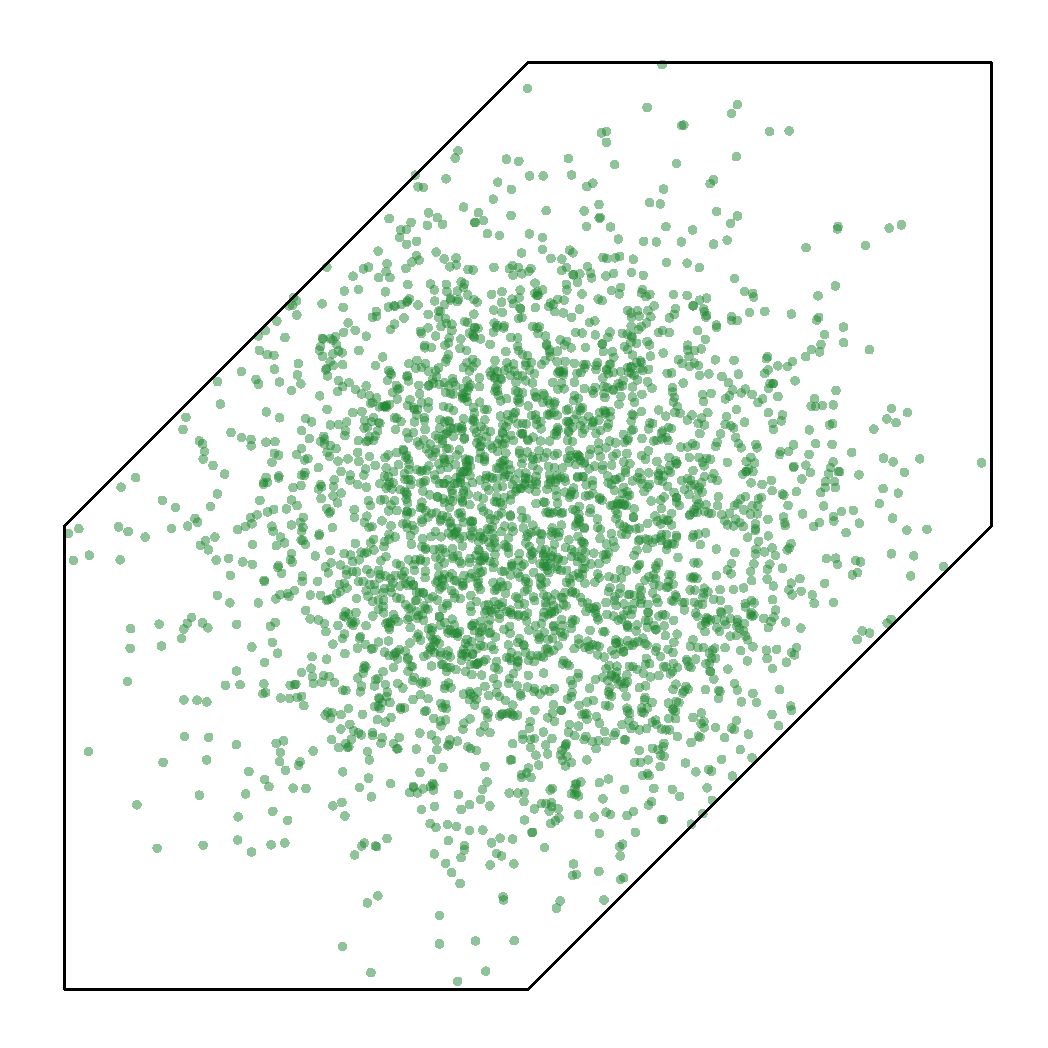
\includegraphics[width=\linewidth]{distr_true_um_norm.pdf}
% %\caption{caption}\label{fig:comparison_a5}
% \end{wrapfigure}% exp_family_maxent.nb
\begin{enumerate}[label=(\roman*)]
\item\label{item:distr_um} Two possible distributions of true utility matrices on the set of \fig~\ref{fig:space_UM} (in that coordinate system): a uniform distribution; and a bivariate (truncated) gaussian distribution centred on the identity matrix $\begin{bsmallmatrix} 1&0\\0&1 \end{bsmallmatrix}$ and with standard deviation $1/3$ in the $x$ and $y$ coordinates of \eqn~\eqref{eq:coords_um}, illustrated in \fig~\ref{fig:gauss_distr_um}.

\item\label{item:distr_cm} A distribution of confusion matrices for which the fraction of one class is uniformly distributed in $\clcl{0,1}$, and the true-positive and true-negative rates are independently distributed in $\clcl{0.5, 1}$ with linearly increasing probabilities (median of 0.85,  lower and upper quartiles at 0.75 and 0.93). This means that we consider problems with highly imbalanced data to be as common as problems with balanced data (a realistic assumption according to our expecience); and candidate classifiers to be generally good.
  
\item\label{item:distr_error} A truncated gaussian distribution of error around each true utility-matrix element, centred on the true utility value. We consider standard deviations ranging from $0$ to $0.3$. The gaussian must be truncated because each true utility has a value between $0$ and $1$ and moreover we require correct classifications to have higher utilities than incorrect ones. Figure~\ref{fig:error_distr_um} illustrates the extent of such an error in the space of utility matrices, for standard deviations equal to $0.1$ and $0.2$.
\end{enumerate}
\begin{figure}[t]
  \centering
  \hspace{\stretch{1}}
  \parbox[t]{0.45\linewidth}{%
    \centering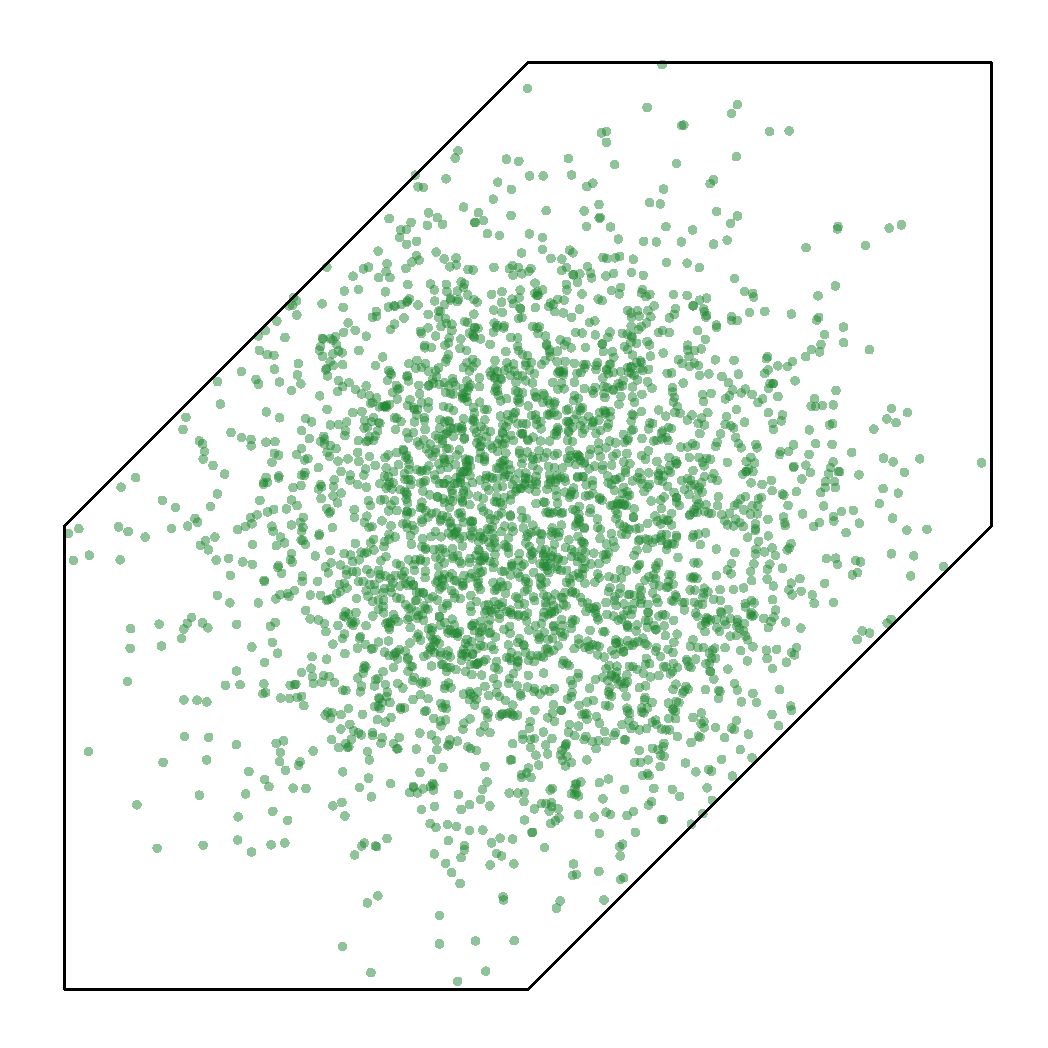
\includegraphics[width=\linewidth]{distr_true_um_norm.pdf}\\
    \caption{Truncated gaussian distribution in the space of utility matrices of \fig~\ref{fig:space_UM}, described in item~\ref{item:distr_um}.}
    \label{fig:gauss_distr_um}}
  \hspace{\stretch{1}}
  \parbox[t]{0.45\linewidth}{%
    \centering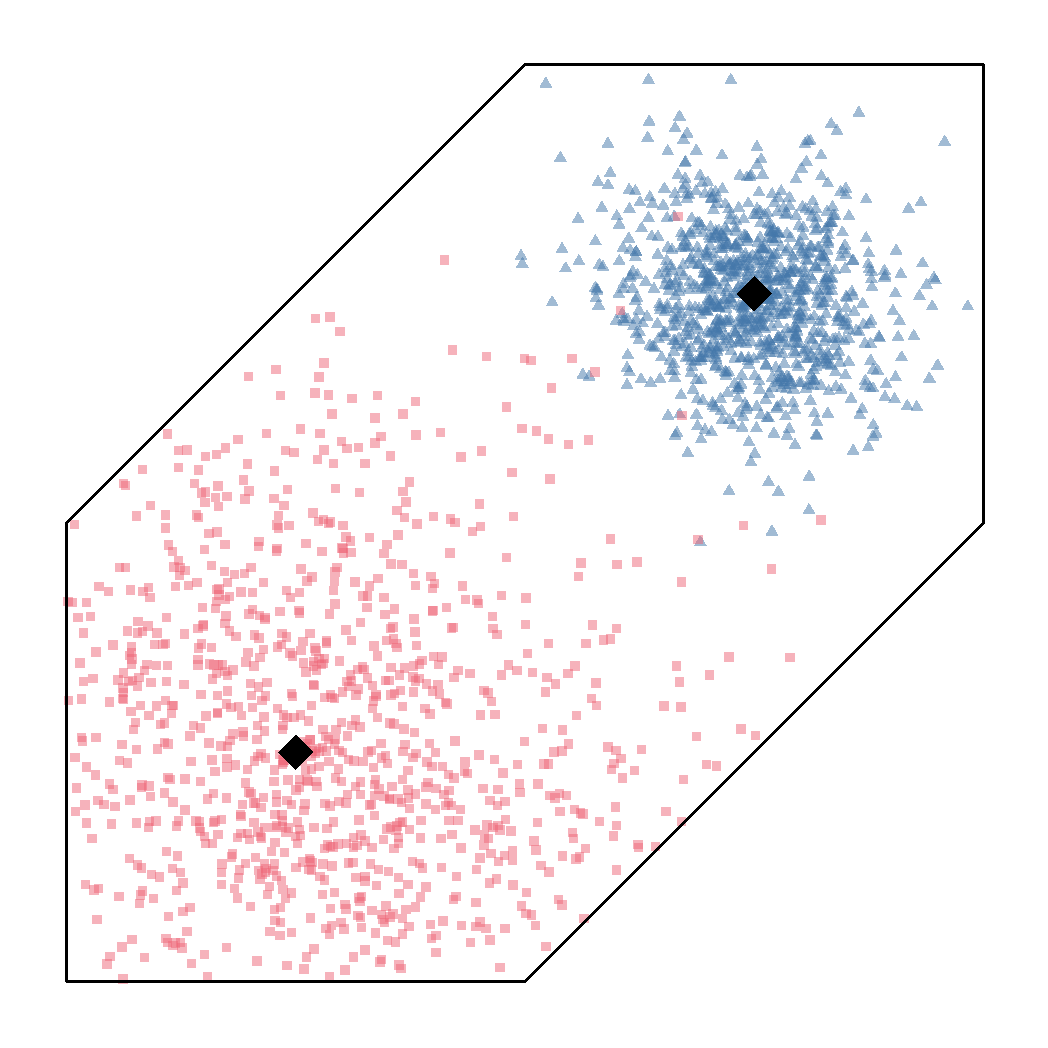
\includegraphics[width=\linewidth]{error_around_um2.pdf}
    \caption{Extents of errors having standard deviations $0.1$ ({\color{mypurpleblue}blue triangles}) and $0.2$ ({\color{myred}red squares}), around the utility matrices $\begin{bsmallmatrix} 0.5&0.5\\0&1 \end{bsmallmatrix}$ and $\begin{bsmallmatrix} 1&0\\0.5&0.1 \end{bsmallmatrix}$ (black diamonds).}
    \label{fig:error_distr_um}}
  \hspace{\stretch{1}}
\end{figure}

Under these assumptions we calculate how often a pair of classifiers, represented by two confusion matrices with the same class proportions, is evaluated in reverse order, with respect to their true utility yield, when an incorrect utility matrix or another metric is used for the evaluation. This calculation is an integration problem that we solve by Monte Carlo sampling. The procedure is intuitive:
\begin{enumerate}[label=\arabic*.,ref=\arabic*]
\item\label{item:draw_um} Select a \enquote{true} utility matrix according to the distribution~\ref{item:distr_um}.
\item\label{item:draw_wrongum} Select errors around the elements of the true utility matrix, according to the distribution~\ref{item:distr_error}, and add them to it.
\item\label{item:draw_cm} Select a class proportion and then two confusion matrices having that class proportion (the class proportion must be the same since the matrices are obtained from the same data), according to the distributions~\ref{item:distr_cm}.
\item\label{item:diff_true} Calculate the difference in the true utility yield of the two confusion matrices, using the true utility from step~\ref{item:draw_um}.
\item\label{item:diff_other} Calculate the difference in
  \begin{enumerate}[label=\theenumi\alph*.]
  \item the scores according to several metrics
  \item the yields according to the erroneous utility matrix from step~\ref{item:draw_wrongum}
  \end{enumerate}
for the two confusion matrices.
\item If the differences from steps~\ref{item:diff_true} and \ref{item:diff_other} disagree in sign then this pair of confusion matrices was incorrectly ranked by the metric or the incorrect utility matrix.
\end{enumerate}

The results of this sampling procedure for the case of uniform distribution of true utility matrices, several metrics, and utilities affected by errors with $0.1$ standard deviation, are shown in \fig~\ref{fig:wrongly_ranked_pairs}.
\begin{figure}[p]
  \centering
    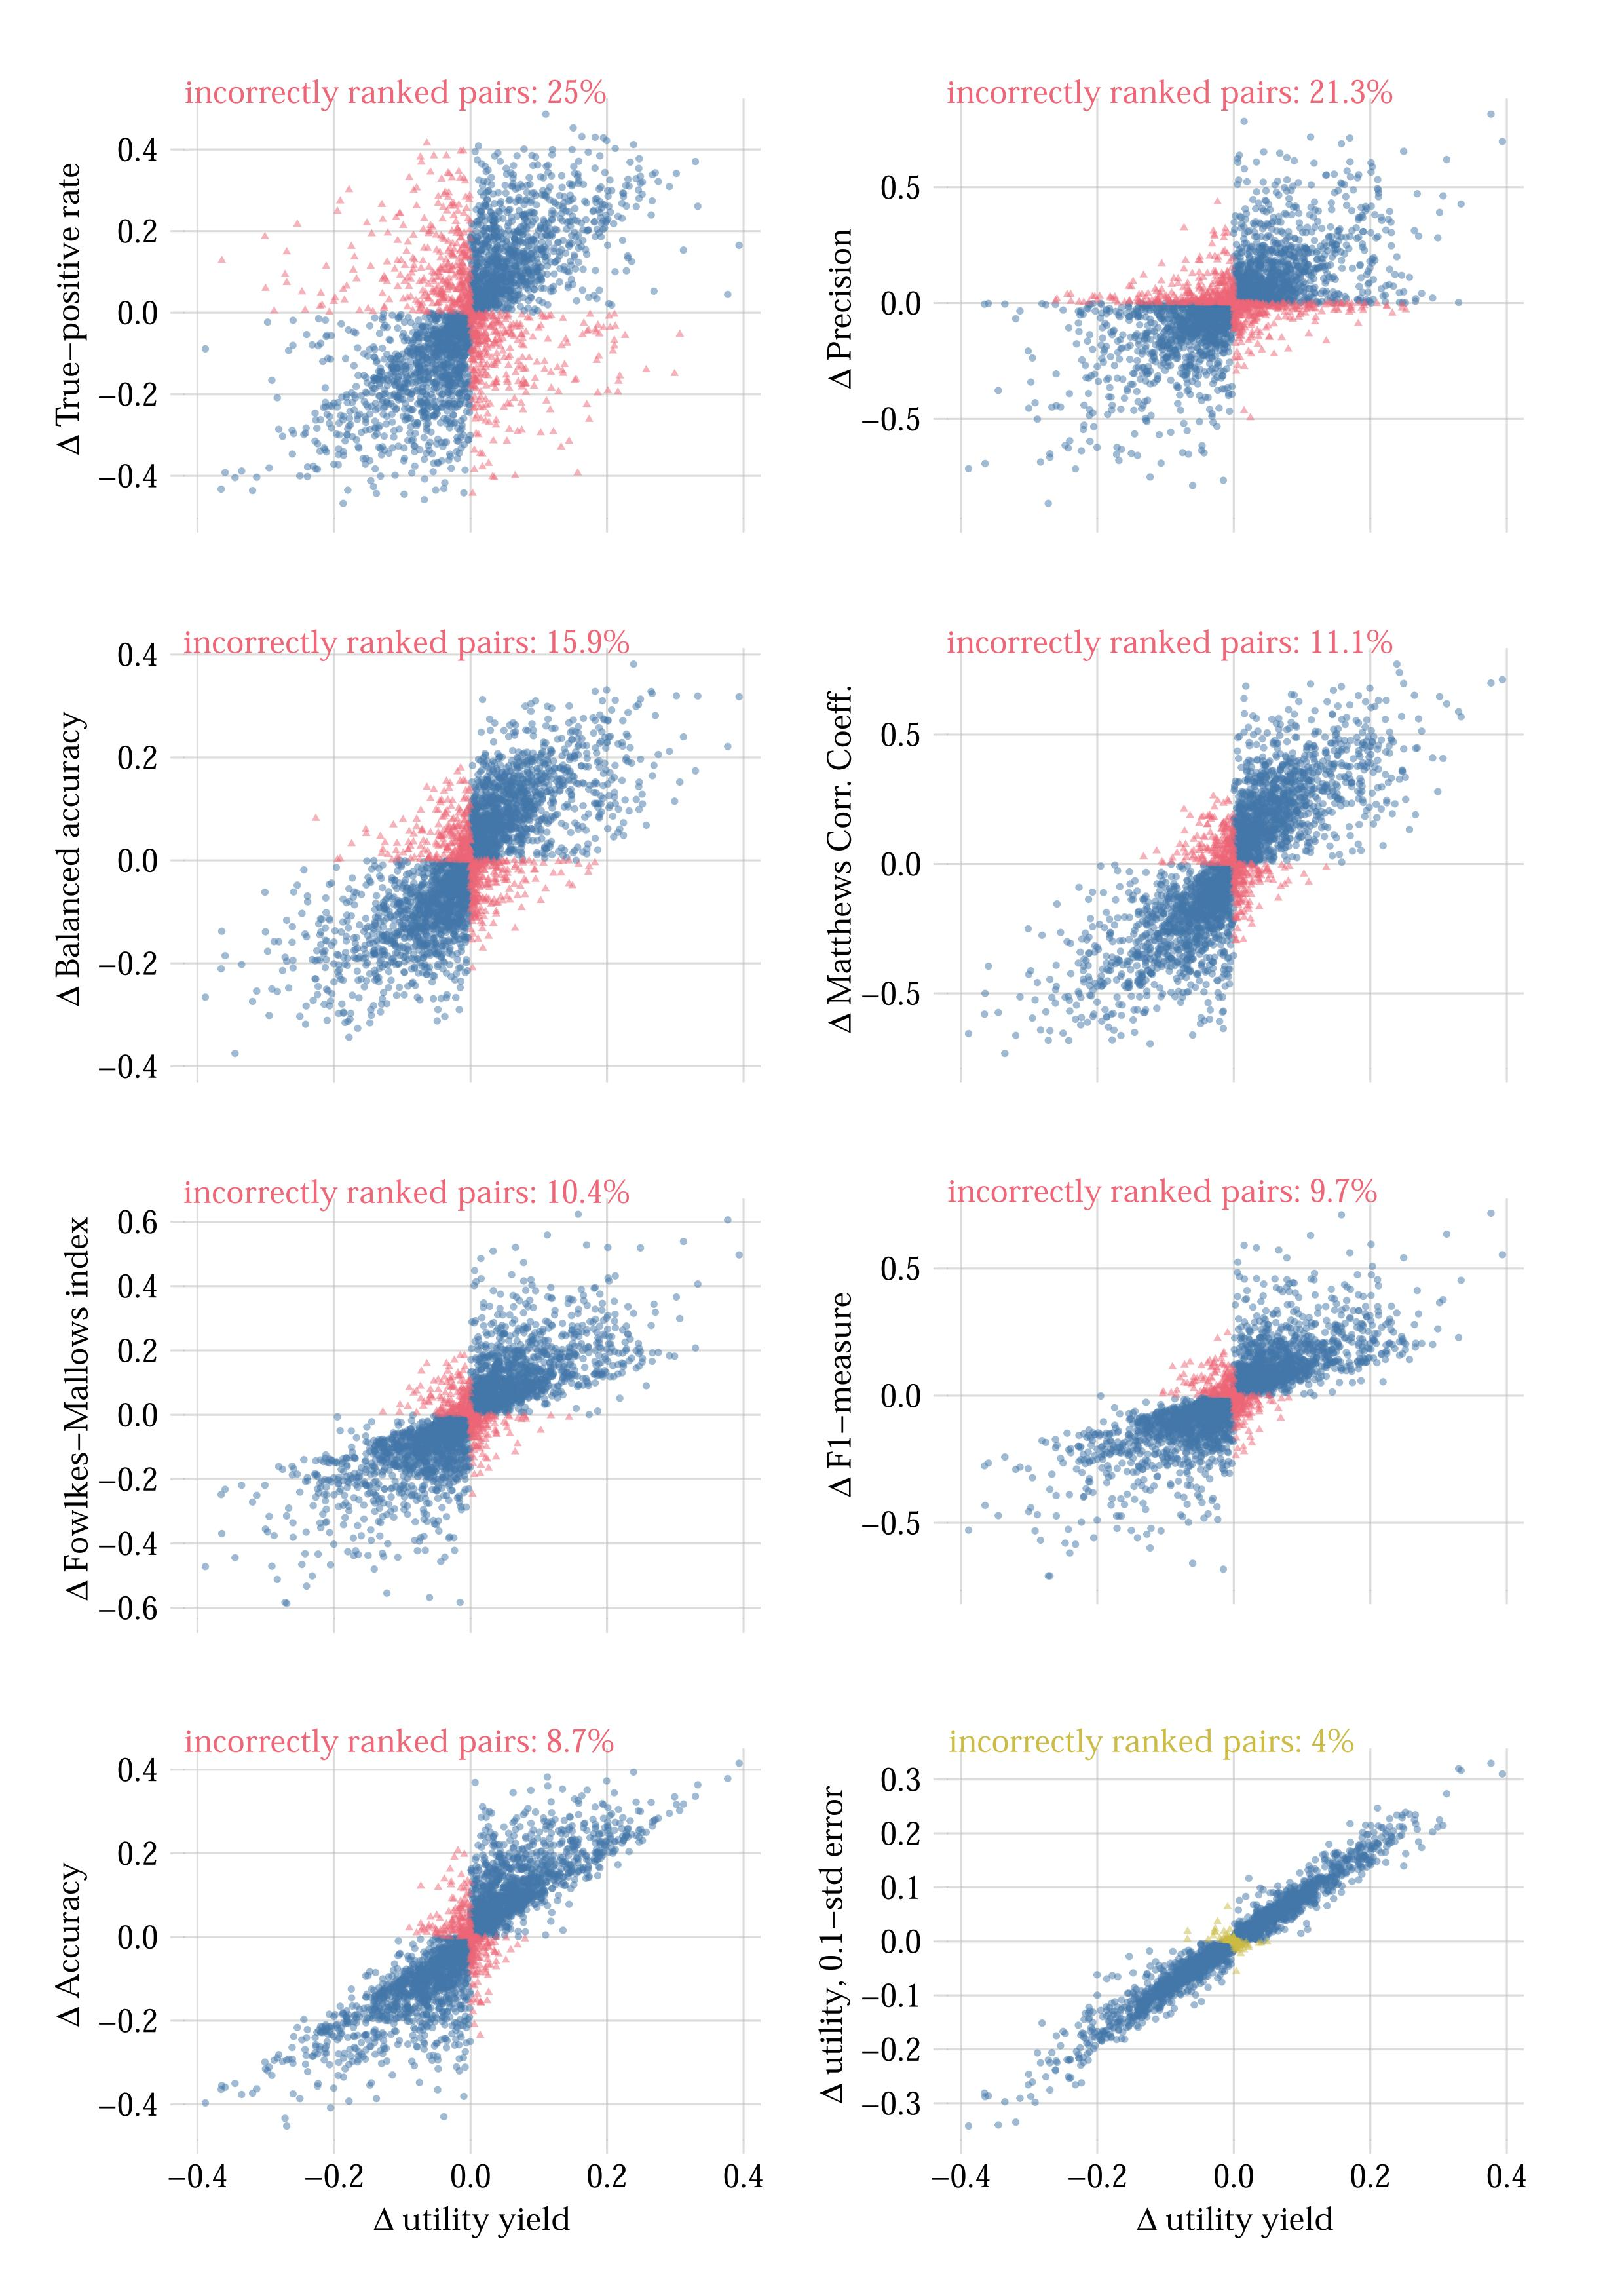
\includegraphics[width=0.99\linewidth]{incorrectscores4unif-11.jpg}\\
  \caption{Relationship between difference in utility yields according to a \enquote{true} utility matrix, and difference in scores according to other metrics including an incorrectly assessed utility matrix (error with $0.1$ standard deviation). Points landing in the II or IV quadrants represent pairs of confusion matrices that were wrongly compared.}
  \label{fig:wrongly_ranked_pairs}
\end{figure}
% %% True-positive/negative rate, not reported: 25.0\% incorrect pair-rankings
% \begin{figure}[p]
%   \centering
%     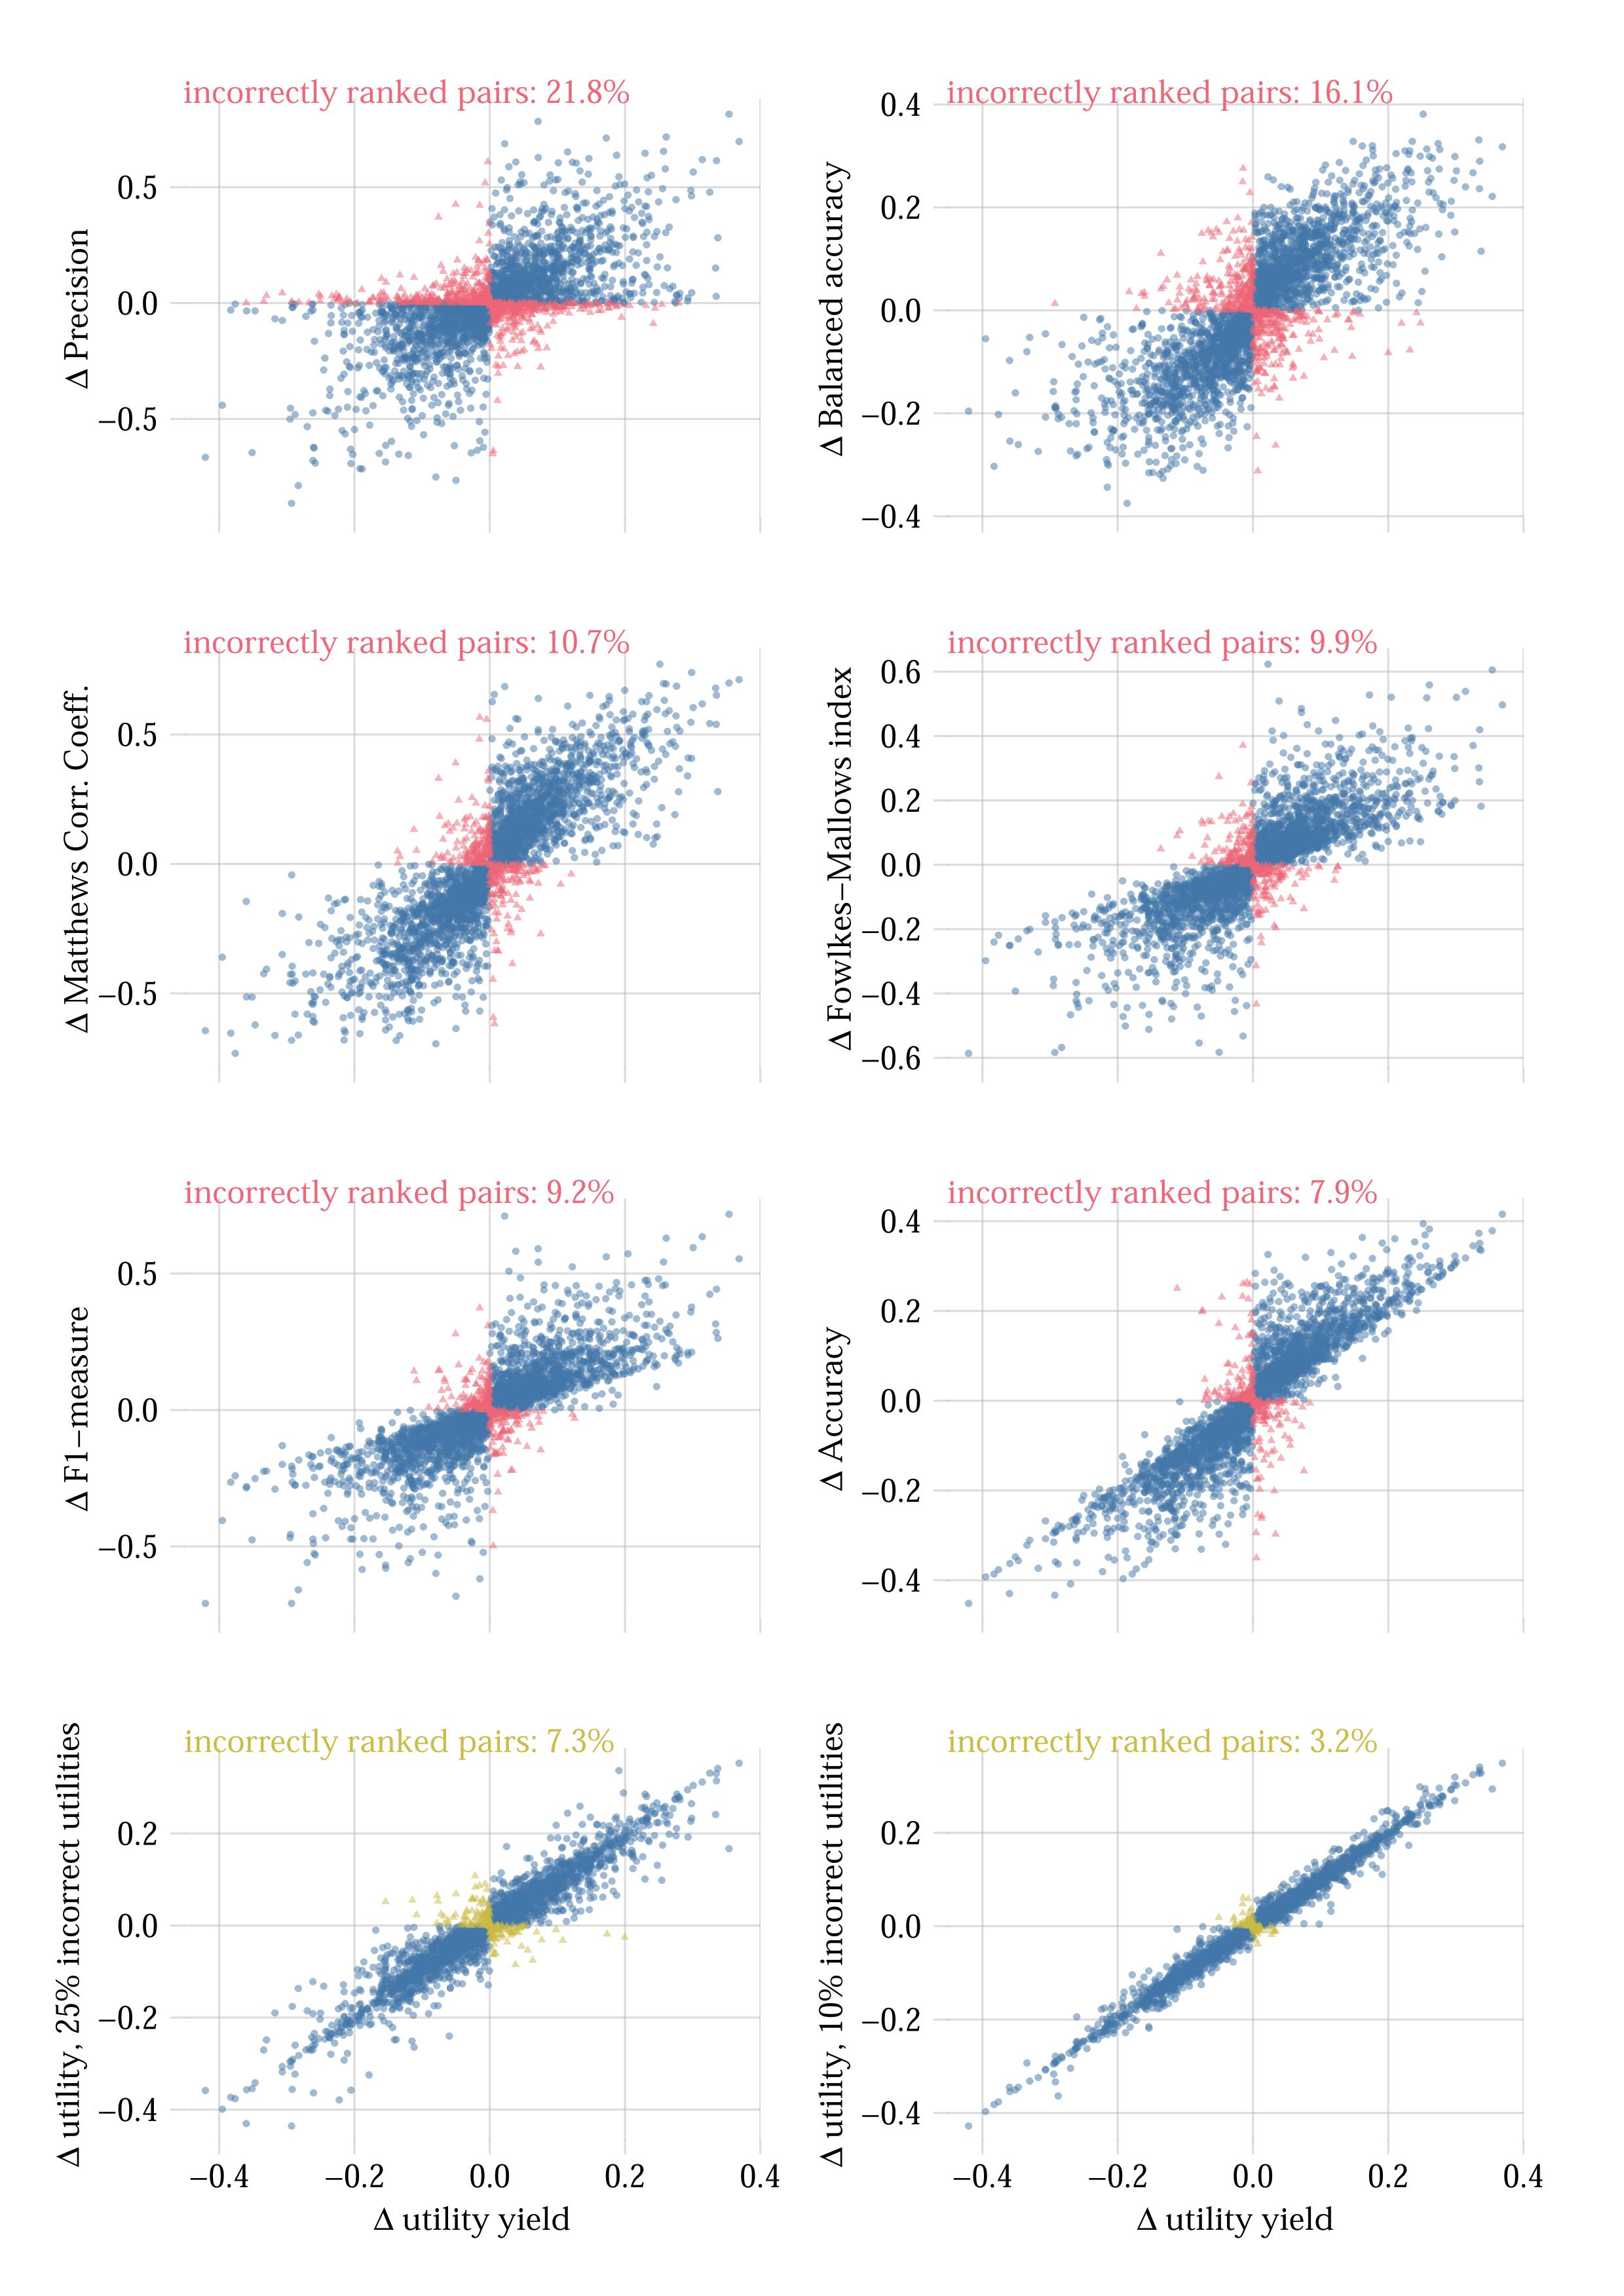
\includegraphics[width=0.99\linewidth]{incorrectscores2norm2_25.jpg}\\
%   \caption{Relationship between various metrics and utility}
%   \label{fig:wrongly_ranked_pairs2}
% \end{figure}
%% True-positive/negative rate, not reported: 25.0\% incorrect pair-rankings
\begin{figure}[p]
  \centering
    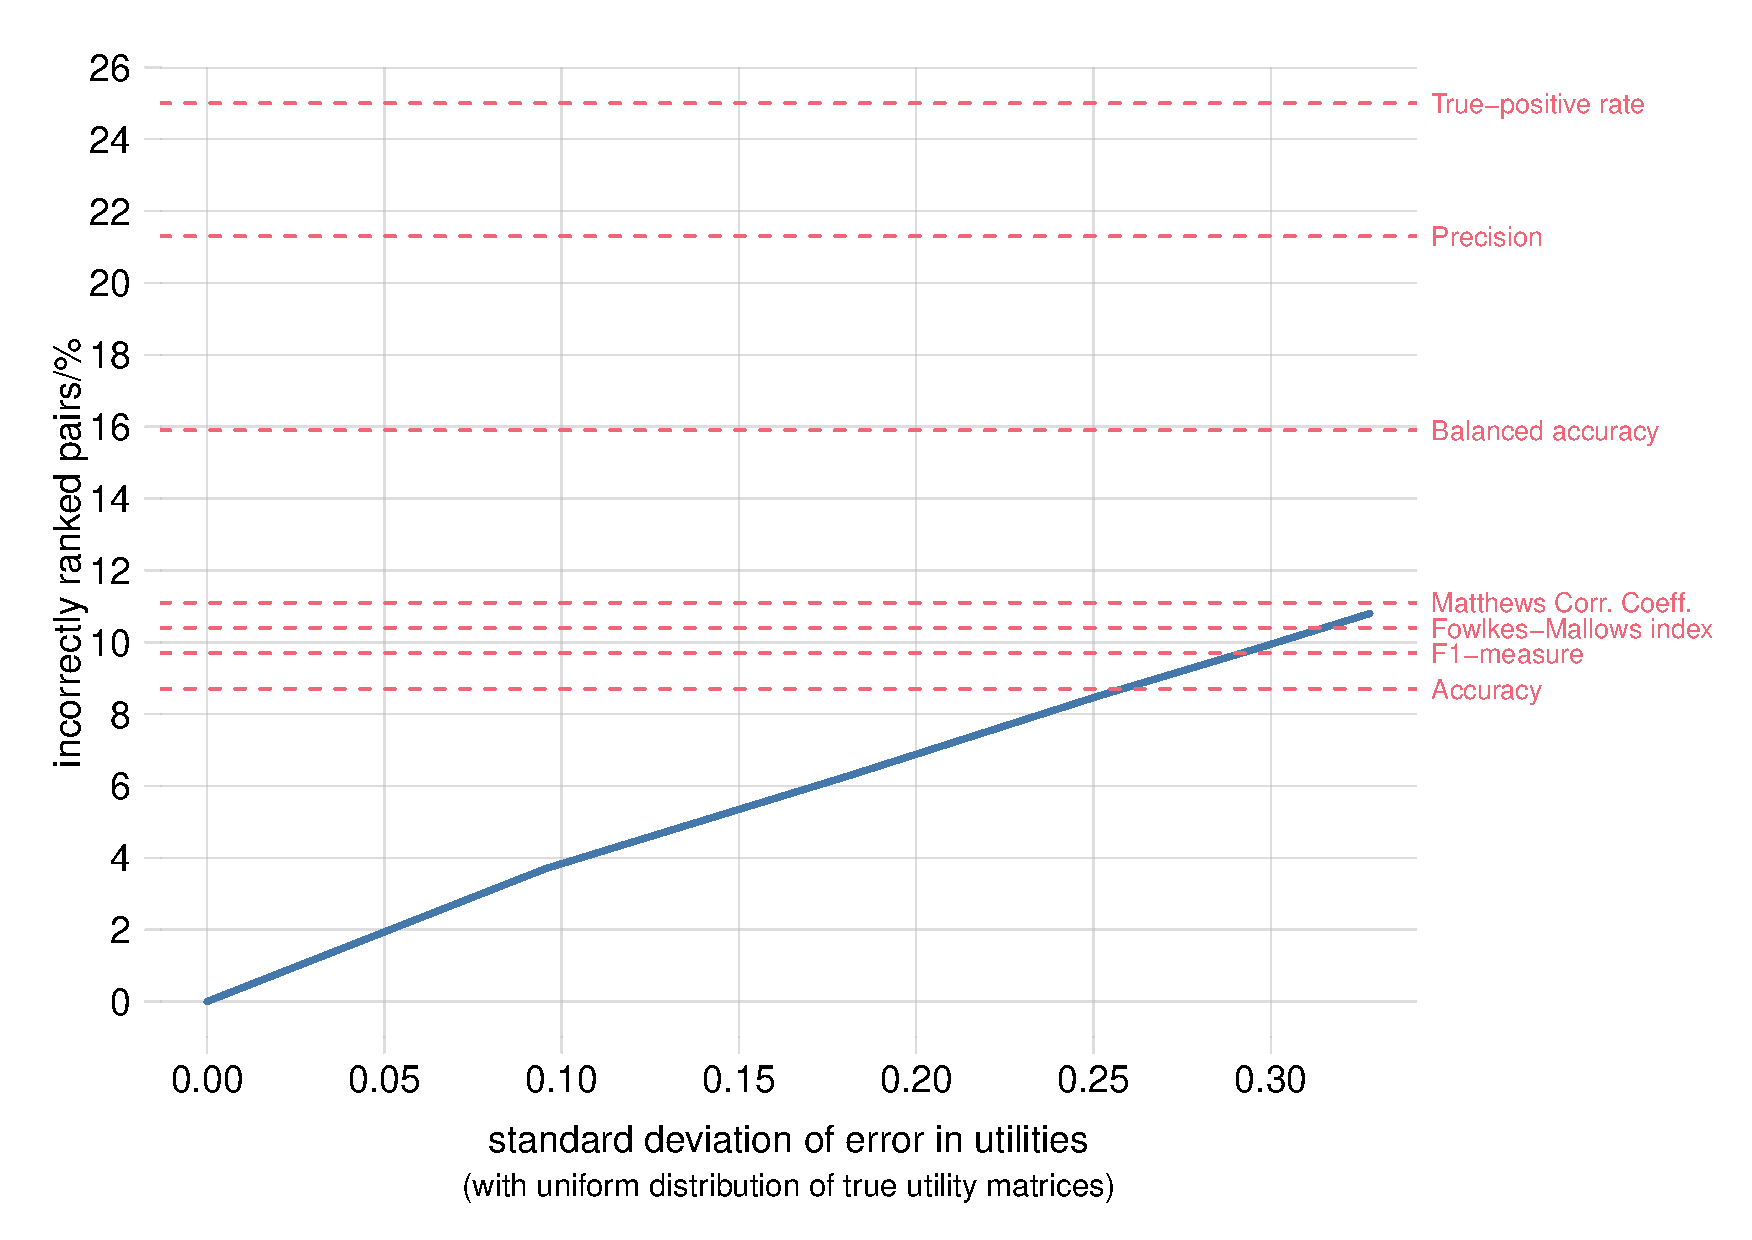
\includegraphics[width=0.99\linewidth]{increase_error2_unif.pdf}\\\hfill
    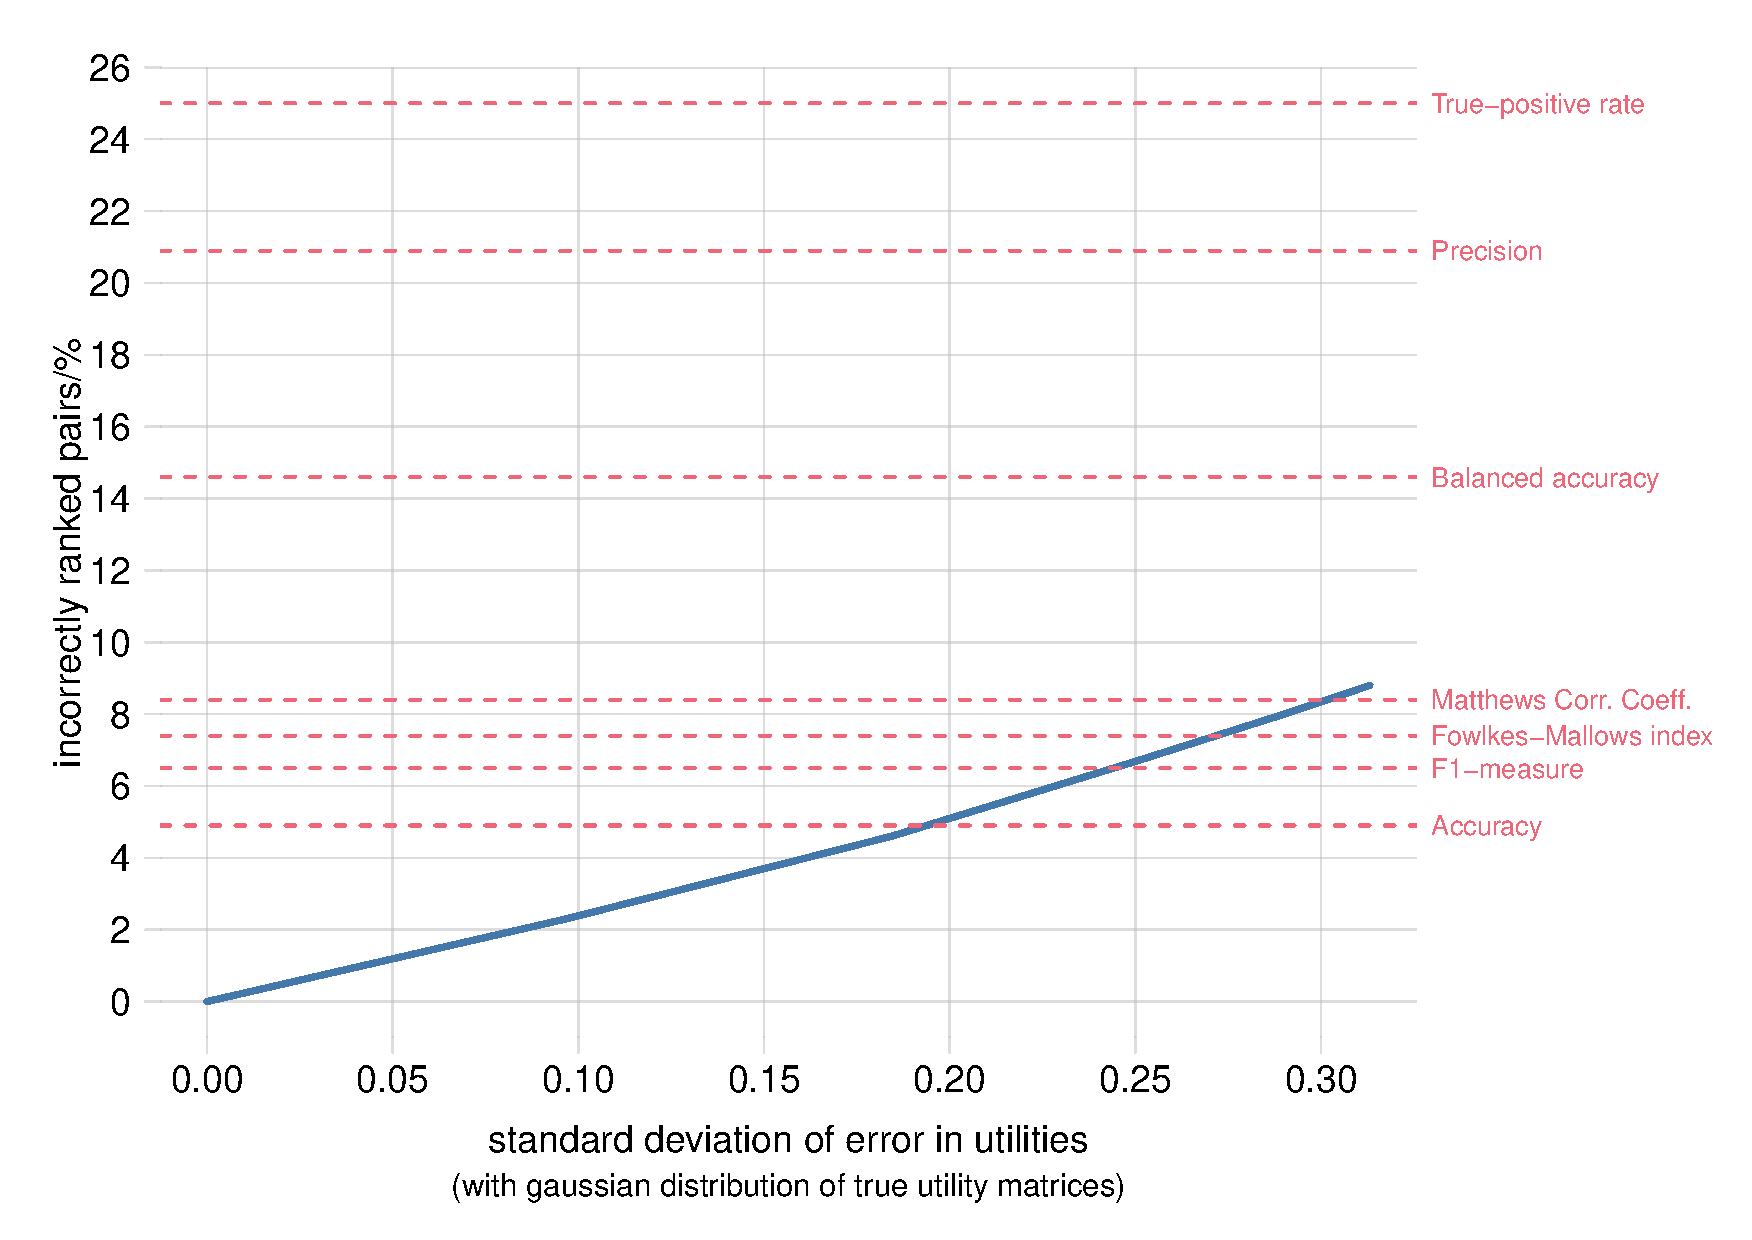
\includegraphics[width=0.99\linewidth]{increase_error2_norm.pdf}\\\hfill
  \caption{Dependence of the proportion of incorrectly ranked pairs of confusion matrices, on the standard deviation of the assessment error on the utilities. Top plot: case with uniform distribution of true utility matrices. Bottom plot: case with gaussian distribution of true utility matrices, as in \fig~\ref{fig:gauss_distr_um}.}
  \label{fig:percentage_vs_error}
\end{figure}
Each point represents a pair of confusion matrices (step~\ref{item:draw_cm}); its coordinates are the true utility yield and either the score given by a metric or (last plot) the yield according to the incorrect utility matrix. The red or yellow triangular points in the in the II and IV quadrants (discordant signs) are incorrectly ranked pairs. The percentages of incorrect rankings are calculated from $10^{6}$ samples, giving slightly more than one decimal significant digit; fewer samples are shown in the plots.

The plots are displayed in order (left-rigt, top-bottom) of decreasing percentages of incorrect rankings. The accuracy metric proves to be the best among the ones considered, leading to $8.7\%$ incorrect pairwise rankings. But we see that a utility matrix affected by gaussian errors with $0.1$ standard deviation is even better, yielding $4\%$ incorrect pairwise rankings.

The dependence of the fraction of incorrect rankings on the standard deviation of the error affecting the utilities is shown in the plots of \fig~\ref{fig:percentage_vs_error}, for the case of uniform distribution (top plot) and gaussian distribution (bottom plot) of true utility matrices. It is approximately linear. The plots also report the fractions of incorrect rankings for the other metrics. We see that evaluations based on a utility matrix affected by errors with standard deviation up to $0.15$ or even $0.25$ are still more reliable than evaluations based on the other reported metrics. This is a remarkable fact, considering that errors with such standard deviations are quite large, as can be seen in \fig~\ref{fig:error_distr_um}.

An utility error with standard deviations around $0.25$ cover the whole space of utility matrices almost uniformly (cf \fig~\ref{fig:error_distr_um}). Such large error means that we were completely uncertain about the utilities to start with. It therefore makes sense that the accuracy, equivalent to using the identity utility matrix, becomes a more reliable metric when this error level is reached. Indeed we saw in \sect~\ref{sec:unknown_utilities} that the identity utility matrix is the natural one to use in a state of complete uncertainty about the utilities.


\section{What about the area under the curve of the receiver operating characteristic?}
\label{sec:auc}

Another very common metric to evaluate binary classifiers is the Area Under the Curve of the Receiver Operating Characteristic, or \enquote{area under the curve} for short. This metric can only be used for particular classifying algorithms, and its meaning is different from that of the metrics reviewed so far. For these reasons we leave a full discussion of it to future works, and only offer a couple of remarks.

The area under the curve can only be computed for classifiers that output a continuous variable rather than a class. A threshold for this variable determines whether its value predicts of one class or the other. Different choices of threshold leads to different pairs of false-positive rate $f$ (which is $1-{}$true-negative rate) and true-positive rate $t$ in a given test set. These pairs can be plotted as a curve $f \mapsto t(f)$ on a graph with corresponding axes. Given the proportion of classes in the test set, every point on such curve corresponds to a possible confusion matrix $C_{ij}(f)$ that the classifier can produce depending on the threshold chosen. The area subtended by such curve is a weighted average of true-positive rates with a peculiar choice of weights; the weights are uniform as a function of false-positive rate, but generally not uniform as a function of the threshold, for example. The meaning and proper use of the receiver operating characteristic are discussed in a classic by \textcites{metz1978}; see especially p.~290.


\medskip

From the standpoint of decision theory two remarks can be made\autocites[similar points are made by][]{bakeretal2001,loboetal2008}. First, according to the principle of maximum expected utility, \sect~\ref{sec:dt_utilities}, we should choose a threshold and corresponding false-positive rate $f^{*}$ such as to maximize the utility yield, given by \eqn~\eqref{eq:final_utility}:
\begin{equation}
  \label{eq:threshold_auc_maxutility}
  \text{\small choose}\quad
  f^{*} = \argmax_{f}\set[\bigg]{\sum_{i,j=0}^{1} U_{ij}\ C_{ij}(f)} \ .
\end{equation}
Any other values of $f$ and of the threshold are irrelevant. Averages over $f$ values are therefore irrelevant as well. Second, if our goal is to evaluate the average performance over several possible classification problems, then the quantities to be averaged are the utility matrices of those classification problems, as discussed in \sect~\ref{sec:unknown_utilities}, yielding a unique expected utility matrix. Once this is computed we go back to a single choice of $f$ according to our first remark.
% Finally, if we wanted to somehow interpret the average implicit in the area under the curve as an average of utility matrices, in accord to the remark above, then such average would depend on the probabilities or frequencies appearing in the confusion matrix, and would therefore imply some sort of cognitive bias as discussed in \sect~\ref{sec:decision_theory}.

Owing to these issues, the area under the curve suffers from the same problems as the non-compliant metrics discussed in \sect~\ref{sec:common_metrics}: in every classification problem it always leads to cases of incorrect evaluation.

A correct use of the receiver-operating-characteristic curve $t(f)$ can be made, however. It is explained in \textcite{metz1978}, section \emph{Cost/Benefit Analysis} p.~295, and in \textcites{soxetal1988_r2013}, \sect~5.7.4 (curiously Sox \etal\ also mention the generally erroneous criterion of the area under the curve).

Denote the proportion of class~$0$ (positive) in the test set by $B$. The confusion matrix as a function of $f$ is then
\begin{equation}
  \label{eq:CM_fromrates}
  \begin{bmatrix}
    C_{00}(f) & C_{01}(f)\\ C_{10}(f) & C_{11}(f)
  \end{bmatrix}
  =
  \begin{bmatrix}
    B\ t(f) & (1-B)\ f \\ B\ [1-t(f)] &(1-B)\ (1-f)
  \end{bmatrix} \ .
\end{equation}
The sum in formula~\eqref{eq:threshold_auc_maxutility} above can then be explicitly written, rearranging some terms,
\begin{multline}
  \label{eq:sum_UC}
    % U_{00}\  B\ t +
    % U_{01}\ (1-B)\ f +
    % U_{10}\ B\ (1-t) +
    % U_{11}\ (1-B)\ (1-f)
  \sum_{i,j=0}^{1} U_{ij}\ C_{ij}(f) \equiv
      (U_{00} - U_{10})\  B\ t(f) -
    (U_{11} - U_{01})\ (1-B)\ f
    +{}\\[-2\jot]
    U_{10}\ B\ + U_{11}\ (1-B) \ .
\end{multline}
The principle of maximum expected utility~\eqref{eq:threshold_auc_maxutility} is  then equivalent to the following condition, obtained using the explicit sum above but dropping the constant term on the second line for simplicity:
\begin{equation}
  \label{eq:threshold_auc_maxutility_rates}
  \text{\small choose}\quad
  f^{*} = \argmax_{f}\set[\big]{
    (U_{00} - U_{10})\  B\ t(f) -
    (U_{11} - U_{01})\ (1-B)\ f
%    + U_{10}\ B\ + U_{11}\ (1-B)
} \ .
  \end{equation}
The function in braces is monotonically increasing because $t(f)$ is (we assume, as always, that the utility of correct classification of a class is higher than that of misclassification, so $U_{00}-U_{10} \ge 0$ and $U_{11}-U_{01} \ge 0$). Its maximum can thus be found by setting its derivative to zero:
\begin{equation}
  \label{eq:threshold_auc_maxutility_derivat}
  \text{\small choose } f^{*} \text{\small\ such that}\quad
t'(f^{*}) = \frac{(U_{11} - U_{01})\ (1-B)}{(U_{00} - U_{10})\  B} \ .
\end{equation}
If we have several classifiers, each with its own curve $t(f)$, then \emph{the best is the one tangent to the line
\begin{equation}
  \label{eq:tangent_line}
  t = \frac{(U_{11} - U_{01})\ (1-B)}{(U_{00} - U_{10})\  B} f + \text{\normalfont\small const.}
\end{equation}
that has the highest intercept.}

From this criterion it can be seen geometrically that if a classifier has its curve $t(f)$ \emph{completely above} the curve of another classifier, then it must have a higher utility yield. But nothing in general can be said if the curves of the two classifiers cross. It is the tangent of a receiver-operating-characteristic curve that matters, not its subtended area. Figure~\ref{fig:auc_example} shows an example of this.
\begin{figure}[t]
  \centering
    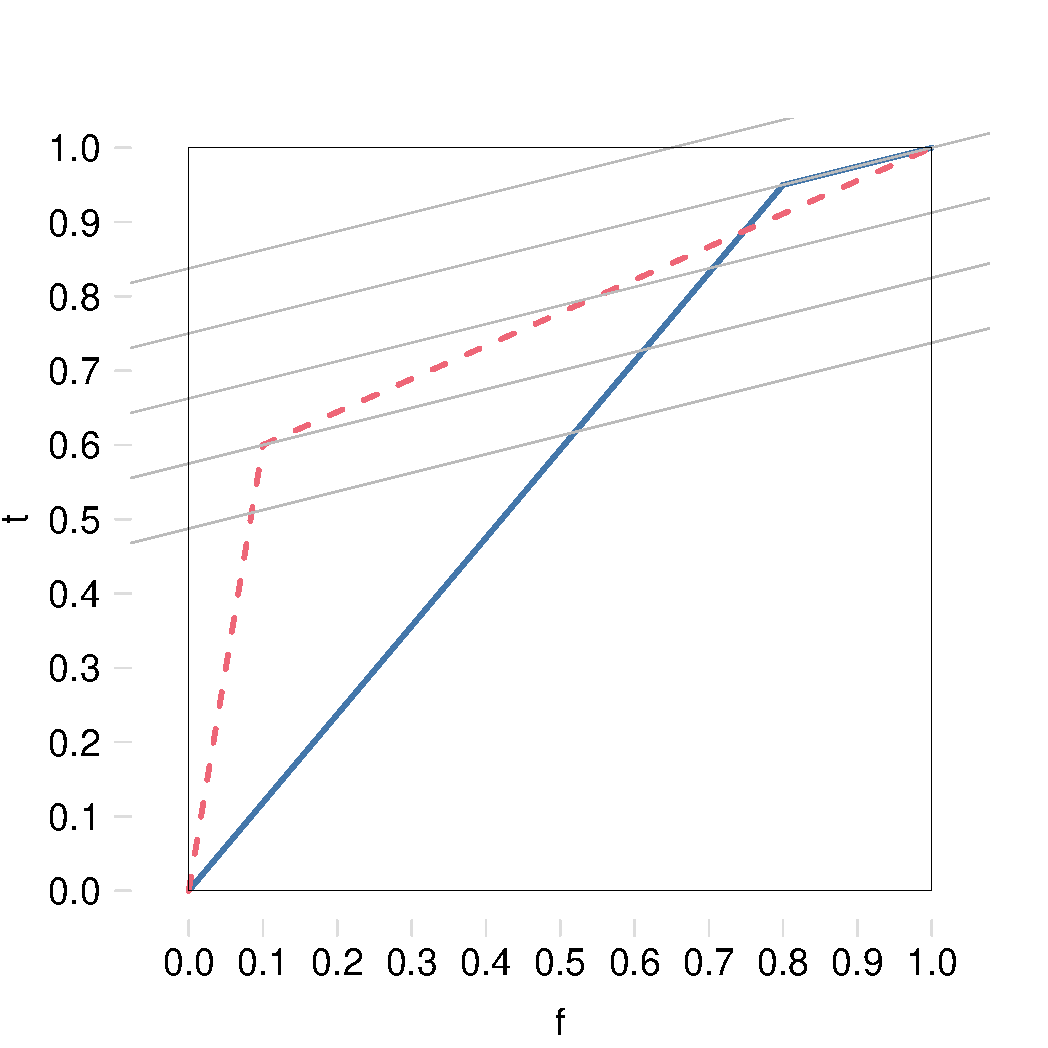
\includegraphics[width=0.66\linewidth]{auc_example.pdf}\\
    \caption{Receiver-operating-characteristic curves of two classifiers. The {\color{red}red dashed curve} clearly subtends a larger area than the {\color{blue}blue solid curve}. Yet the classifier with the latter curve yields a higher utility, because it touches the family of parallel lines, \eqn~\eqref{eq:tangent_line}, at a higher point. This example arises for a utility matrix equal to $\begin{bsmallmatrix} 4&0\\0&1 \end{bsmallmatrix}$ and a test set with $B=0.5$ (balanced), or for a utility matrix equal to $\begin{bsmallmatrix} 1&0\\0&1 \end{bsmallmatrix}$ and a test set with $B=0.8$.}
  \label{fig:auc_example}
\end{figure}






% \section{Remarks on the choice of test dataset}
% \label{sec:test_set}
%
% It may not be amiss to emphasize that the \emph{proportions $N_{c}$ of classes in the test set should be representative of the proportions that will be encountered in the real application}. Otherwise the test-set results would misleading or even opposite to what the real performance will be. In the lottery example with utility matrix~\eqref{eq:exp_utilities_lottery}, suppose we have an algorithm that always makes the decision \texttt{buy} and another algorithm that always decides \texttt{not-buy}. In  real instances of such lotteries the class \texttt{win} occurs 1\% of the time, and \texttt{lose}, 99\%. In a real application the first algorithm would thus yield $-0.89$, a loss, on average at each instance, and the second $0$. The second algorithm is actually best. Suppose we test these algorithms on a test set where the two classes appear 50\%/50\% instead. On this test set the first algorithm will yield $4.5$ on average, the second $0$. Thus according to the test the first algorithm is best -- a wrong conclusion.




\section{Summary and discussion}
\label{sec:discussion}

The evaluation and ranking of classification algorithms is a critical stage in their development and deployment. Without such evaluation we cannot even say whether an algorithm is better than another, or whether a set of parameter values for a specific algorithm is better than another set.

And yet at present we have not an evaluation theory, but only an evaluation folklore: different procedures, proposed only out of intuition and of analysis of special cases, with fuzzy criteria to decide which should be used, and without rigorous theoretical foundations that should guarantee uniqueness and universality properties and absence of biases. We believe that some of the surprising failures of machine-learning \emph{in actual applications}\autocites[see \eg][]{varoquauxetal2022} come not only from biases in the choice of test datasets and similar biases, but also from the use of wrong evaluation metrics.

In the present work we have argued that theoretical foundations for the evaluation process are available in \emph{decision theory}. Its main notions and principle -- utilities and their maximization -- are very intuitive, as shown (we hope) by the introductory story.

These are the main results of the application of decision theory to the evaluation of classifiers:
\begin{itemize}[--,wide]
\item The evaluation metric depends on the specific classification problem.
\item Such metric is completely defined by $n^{2}$ parameters, called utilities, collected in a utility matrix; $n$ is the number of classes. Two parameters are arbitrary and represent a zero and measurement unit of the utility scale. In the binary-classification case this means that we have a two-dimensional set of possible metrics.
\item A utility matrix also appears when we are uncertain about the utilities underlying a classification problem, or when we want to consider the average performance over several classification problems.
\item The score of a classifier on a test set is simply given by its utility yield: the grand sum of the products of the elements of the utility matrix and the confusion matrix of the classifier. It is therefore a simple linear expression in the confusion matrix elements.
\item Some popular metrics such as precision, balanced accuracy, Matthews correlation coefficient, Fowlkes-Mallows index, $F_{1}$-measure, and area under the receiver-operating-characteristic curve do not comply with decision theory. As a consequence they are affected by cognitive biases and always lead to some erroneous comparative evaluations of classifiers in every classification problem.
\item Using a utility matrix with incorrectly assessed utilities still leads on average to fewer wrong comparative evaluations than using other popular metrics.
\end{itemize}

We believe that the decision-theoretic evaluation of classifiers has remarkable advantages.

First, it translates the fuzzy problem \enquote*{which of the numerous scores should I rely on?} into a more structured, thus easier to confront, one: to assess, at least semi-quantitatively, how many times more valuable, desirable, or useful is the correct classification of a class than its incorrect classification, than the correct classification of another class, and so on. Such utilities usually have a more immediate, problem-dependent interpretation than other metrics.

Second, it leads to a mathematically extremely simple, computationally convenient metric: a linear combination of confusion-matrix elements. No need of transcendental functions or of the integration of curves.

Third, the principles of the underlying theory guide us if we have to face new peculiar problems. Imagine for instance a classification problem where we cannot say, in general, whether true positives are more important than true negatives and so on, because such valuation can vary from one tested item to another. Decision theory in this case requires an item-wise assessment of utilities, and still provides an item-wise score, which can be accumulated across items to obtain a total evaluation score for the performance of candidate classifiers.


% \mynotep{We recommend to avoid metrics not complying with decision theory -- not of the form~\eqref{eq:general_valuation_metric} -- and to try to get an estimate of the utilities involved instead.}








%%%% examples use empheq
%   \begin{empheq}[left={\mathllap{\begin{aligned}    \de\yF_{\yc}/\de\yp&=0\text{:} \\
%         \de\yF_{\yc}/\de\ym&=0\text{:}\\ \de\yF_{\yc}/\de\yl&=0\text{:}\end{aligned}}\qquad}\empheqlbrace]{align}
%     \label{eq:con_p}
% %    \de\yF_{\yc}/\de\yp &\equiv
%     -\ln\yp + \ln\yq + \yl\yM + \ym\yu &=0,\\
%     \label{eq:con_u}
% %    \de\yF_{\yc}/\de\ym &\equiv
%     \yu\yp-1 &=0,\\
%     \label{eq:con_l}
%     %\de\yF_{\yc}/\de\yl &\equiv
%     \yM\yp-\yc &=0.
%   \end{empheq}
%%%%
% \begin{empheq}[box=\widefbox]{equation}
%   \label{eq:maxent_question}
%   \p\bigl[\yE{N+1}{k} \bigcond \tsum\yo\yf{N}\in\yA, \yM\bigr] = \mathord{?}
% \end{empheq}


%%\setlength{\intextsep}{0ex}% with wrapfigure
%%\setlength{\columnsep}{0ex}% with wrapfigure
%\begin{figure}[p!]% with figure
%\begin{wrapfigure}{r}{0.4\linewidth} % with wrapfigure
%  \centering\includegraphics[trim={12ex 0 18ex 0},clip,width=\linewidth]{maxent_saddle.png}\\
%\caption{caption}\label{fig:comparison_a5}
%\end{figure}% exp_family_maxent.nb


%%%%%%%%%%%%%%%%%%%%%%%%%%%%%%%%%%%%%%%%%%%%%%%%%%%%%%%%%%%%%%%%%%%%%%%%%%%%
%%% Acknowledgements
%%%%%%%%%%%%%%%%%%%%%%%%%%%%%%%%%%%%%%%%%%%%%%%%%%%%%%%%%%%%%%%%%%%%%%%%%%%% 
\begin{acknowledgements}
  PGLPM thanks Maja, Mari, Miri, Emma for continuous encouragement and affection;  Buster Keaton and Saitama for filling life with awe and inspiration; and the developers and maintainers of \LaTeX, Emacs, AUC\TeX, Open Science Framework, R, Python, Inkscape, LibreOffice, Sci-Hub for making a free and impartial scientific exchange possible.
  % Our work was supported by the Trond Mohn Research Foundation, grant number BFS2018TMT07
%\rotatebox{15}{P}\rotatebox{5}{I}\rotatebox{-10}{P}\rotatebox{10}{\reflectbox{P}}\rotatebox{-5}{O}.
%\sourceatright{\autanet}
%\mbox{}\hfill\autanet
\end{acknowledgements}

%%%%%%%%%%%%%%%%%%%%%%%%%%%%%%%%%%%%%%%%%%%%%%%%%%%%%%%%%%%%%%%%%%%%%%%%%%%%
%%% Appendices
%%%%%%%%%%%%%%%%%%%%%%%%%%%%%%%%%%%%%%%%%%%%%%%%%%%%%%%%%%%%%%%%%%%%%%%%%%%% 
%\clearpage
% \bigskip
% \renewcommand*{\appendixpagename}{}
% % \renewcommand*{\appendixname}{Appendix: test2}
% % %\appendixpage
% \appendix



%%%%%%%%%%%%%%%%%%%%%%%%%%%%%%%%%%%%%%%%%%%%%%%%%%%%%%%%%%%%%%%%%%%%%%%%%%%%
%%% Bibliography
%%%%%%%%%%%%%%%%%%%%%%%%%%%%%%%%%%%%%%%%%%%%%%%%%%%%%%%%%%%%%%%%%%%%%%%%%%%% 
\renewcommand*{\finalnamedelim}{\addcomma\space}
\defbibnote{prenote}{{\footnotesize (\enquote{de $X$} is listed under D,
    \enquote{van $X$} under V, and so on, regardless of national
    conventions.)\par}}
% \defbibnote{postnote}{\par\medskip\noindent{\footnotesize% Note:
%     \arxivp \mparcp \philscip \biorxivp}}

\printbibliography[prenote=prenote%,postnote=postnote
]

\end{document}

%%%%%%%%%%%%%%%%%%%%%%%%%%%%%%%%%%%%%%%%%%%%%%%%%%%%%%%%%%%%%%%%%%%%%%%%%%%%
%%% Cut text (won't be compiled)
%%%%%%%%%%%%%%%%%%%%%%%%%%%%%%%%%%%%%%%%%%%%%%%%%%%%%%%%%%%%%%%%%%%%%%%%%%%% 

\mynotez{[Luca] I find it very difficult to structure the paper: there seems to be issues at several levels in the development and use of binary classifiers (and classifiers in general) within machine-learning.

  Here are some relevant points:
  \begin{itemize}
  \item There should be a distinction between \enquote{inference} (or forecast, prediction, guess) and \enquote{decision} (or action, choice). In particular, the possible situations we may be uncertain about and the possible decisions available may be completely different things. A clinician, for example, may be uncertain about \enquote{cancer} vs \enquote{non-cancer}, while the choices are about \enquote{drug treatment 1} vs \enquote{drug treatment 2} vs \enquote{surgery}.

  \item Probability theory \amp\ decision theory say that in order to make self-consistent decision we need two things: (a) the probabilities for the possible situations, (b) the utilities of the decisions given each possible situation.

  \item A useful \ml\ algorithm should therefore give us one of two things:
\begin{itemize}
\item either the \emph{probabilities} of the uncertain situations
  (\enquote{cancer} vs \enquote{non-cancer} in the example above),
\item or the final decision (\enquote{drug treatment 1} vs \enquote{drug
    treatment 2} vs \enquote{surgery} in the example above).
\end{itemize}
Current \ml\ classifiers do not give us either: the output in the example
above would be \enquote{cancer} vs \enquote{non-cancer}, often without
probabilities.

\item So there are two possible solutions to the problem above:
  \begin{itemize}
  \item We must build a classifier that outputs probabilities. The 0--1
    outputs of current classifiers cannot properly interpreted as
    probabilities, for various reasons.
  \item We must build a classifier that output \emph{decisions}: so not
    \enquote{cancer} vs \enquote{non-cancer}, but \enquote{drug treatment
      1} vs \etc.
  \end{itemize}

\end{itemize}
}


\mynotez{[maybe the following discussion is unnecessary:]
  
Several conventions can be used to fix the two redundant degrees of freedom. We can choose them in such a way that the smallest utility is 0 and the largest is 1; this is achieved by subtracting the value of the smallest utility from all elements of the utility matrix and then dividing them by the value of the largest minus the smallest; in symbols
\begin{equation}
  \label{eq:standardize1}
  U_{cd} \mapsto \frac{U_{cd} - \min(U_{cd})}{\max(U_{cd}) - \min(U_{cd})} \ .
\end{equation}
In the lottery example this leads to
\begin{equation}
  \label{eq:standardize1_lottery}
  \begin{pmatrix}
    +10 & -1 \\ 0 & 0
  \end{pmatrix} \mapsto
    \begin{pmatrix}
    1 & 0 \\ 1/11 & 1/11
  \end{pmatrix} \ .
\end{equation}
Another convention is to choose them in such a way that the smallest utility is 0 and the sum of all utilities is 1; this is achieved by the transformation
\begin{equation}
  \label{eq:standardize2}
  U_{cd} \mapsto
  \frac{U_{cd} - \min(U_{cd})}{\sum_{cd}U_{cd} - \nd\nc\min(U_{cd})} \ .
\end{equation}
In the lottery example this leads to
\begin{equation}
  \label{eq:standardize1_lottery}
  \begin{pmatrix}
    +10 & -1 \\ 0 & 0
  \end{pmatrix} \mapsto
    \begin{pmatrix}
    11/13 & 0 \\ 1/13 & 1/13
  \end{pmatrix} \ .
\end{equation}
}

%%%%%%%%%%%%%%%%%%%%%%%%%%%%%%%%%%%%%%%%%%%%%%%%%%%%%%%%%%%%%%%%%%%%%%%%%
%%%% other cut text

\clearpage

\bigskip
\mynotew{\hrule
  
Pieces from old version below

\hrule}




\subsection{Actual utility yield}
\label{sec:dt_utility_yield}

The utility matrix is not only the basis for making optimal decisions by means of expected-utility maximization. It also provides the metric to rank a set of decisions already made -- for example on a test set -- by some algorithm, if we know the corresponding true classes. Suppose we have $N$ test instances, in which each class $c$ occurs $N_{c}$ times, so that $\sum_{c} N_{c} = N$. A decision algorithm made decision $d$ when the true class was $c$ a number $M_{dc}$ of times. These numbers form the confusion matrix $(M_{dc})$ of the algorithm's output. The numbers $M_{dc}$ are must satisfy the constraints $\sum_{d} M_{dc} = N_{c}$ for each $c$.

For given decision $d$ and class $c$, in each of the $M_{dc}$ instances the algorithm yielded a utility $U_{dc}$. The actual average utility yield in the test set is then
\begin{equation}
  \label{eq:utility_gained}
 \frac{1}{N} \sum_{dc} U_{dc}\, M_{dc} \ .
\end{equation}
It is convenient to consider the average utility yield, rather than the total utility yield (without the $1/N$ factor), because if we shift the zero or change the measurement unity of our utilities then the yield changes in the same way.



% The utility matrix is not only the basis for making optimal decisions by means of expected-utility maximization. It also provides the metric to rank a set of decisions already made -- for example on a test set -- by some algorithm, if we know the corresponding true classes. Suppose we have $N$ test instances, in which each class $c$ occurs $N_{c}$ times, so that $\sum_{c} N_{c} = N$. A decision algorithm made decision $d$ when the true class was $c$ a number $M_{dc}$ of times. These numbers form the confusion matrix $(M_{dc})$ of the algorithm's output. The numbers $M_{dc}$ are not all independent: they must satisfy the constraints
% \begin{equation}
%   \label{eq:sum_frequencies}
%   \sum_{d} M_{dc} = N_{c} \quad\text{for each class $c$} \ .
% \end{equation}
% The test output of the decision algorithm is therefore characterized by $(\nd-1)\nc$ independent numbers. We can take these to be the first $\nd-1$ rows of the confusion matrix, so that for the last row we have
% \begin{equation}
%   \label{eq:lastrow_conf_matrix}
%   M_{\nd c} = N_{c} - \sum_{d=1}^{\nd - 1} M_{dc}
%   \quad\text{for each class $c$} \ .
% \end{equation}
% In binary classification for example, where $\nd=\nc=2$, the two independent numbers are often taken to be the \enquote{true positives} and \enquote{false positives} (the axes of the receiver-operating-characteristic plot).

% For given decision $d$ and class $c$, in each of the $M_{dc}$ instances the algorithm yielded a utility $U_{dc}$. The actual total utility gained in the test set is then
% \begin{equation}
%   \label{eq:utility_gained}
%   \sum_{d=1}^{\nd}\sum_{c=1}^{\nc} U_{dc}\, M_{dc}
%   \quad\text{or}\quad
%   \sum_{d=1}^{\nd  - 1}\sum_{c=1}^{\nc} (U_{dc} - U_{\nd c})\, M_{dc}
%   + \sum_{c=1}^{\nc} U_{\nd c}\,N_{c}
%    \ ,
%   % \sum_{d=1}^{\nd}\sum{c=1}^{\nc} U_{dc}\, M_{dc}
%   % \sum_{d=1}^{\nd-1}\sum{c=1}^{\nc} U_{dc}\, M_{dc}
%   % + \sum_{c=1}^{\nc} U_{\nd c}\,M_{\nd c}
%   % \sum_{d=1}^{\nd-1}\sum{c=1}^{\nc} U_{dc}\, M_{dc}
%   % + \sum_{c=1}^{\nc} U_{\nd c}\,(N_{c} - \sum_{d=1}^{\nd-1}M_{d c})
%   % \sum_{d=1}^{\nd-1}\sum{c=1}^{\nc} U_{dc}\, M_{dc}
%   % + \sum_{c=1}^{\nc} U_{\nd c}\,N_{c}
%   % - \sum_{c=1}^{\nc}\sum_{d=1}^{\nd-1} U_{\nd c}\,M_{dc})
% \end{equation}
% the second expression being in terms of the independent elements of the confusion matrix. We can also consider the average gained utility per test instance:
% \begin{equation}
%   \label{eq:avg_utility_gained}
%   \sum_{d=1}^{\nd}\sum_{c=1}^{\nc} U_{dc}\, \frac{M_{dc}}{N}
%   \quad\text{or}\quad
%   \sum_{d=1}^{\nd  - 1}\sum_{c=1}^{\nc} (U_{dc} - U_{\nd c})\, \frac{M_{dc}}{N}
%   + \sum_{c=1}^{\nc} U_{\nd c}\,\frac{N_{c}}{N} \ .
% \end{equation}

% [Don't know whether to include the following discussion, it may not have substantial import in this work]
% Formulae~\eqref{eq:utility_gained} or \eqref{eq:avg_utility_gained} show that the performance and ranking of several decision algorithm depend on the values of the utility matrix $(U_{dc})$, and that changes in the zero or measurement unit of the utilities do not affect such raking, as it should intuitively be the case. Note, however, that two \emph{in}equivalent utility matrices can also lead to the same ranking, \emph{provided the frequencies $N_{c}$ of the classes are not changed}. If we add a different constant term to each column of the utility matrix, these terms disappear within the parentheses of formulae~\eqref{eq:utility_gained} and \eqref{eq:avg_utility_gained} and only contribute a total constant term in the remaining sum. This happens because the performance depends not only on the utility but also on the relative proportions of classes.


\bigskip

The summary of decision theory just given suffices to address issues~\ref{item:metrics}--\ref{item:optimal_true}.





\bigskip

In comparing, evaluating, and using \ml\ classifiers we face a number of questions and issues; some are well-known, others are rarely discussed:

\begin{enumerate}[label=\textbf{\textsf{i\arabic*}},ref=\textbf{\textsf{i\arabic*}},itemsep=\parsep]
  
\item\label{item:metrics}\textsf{\textbf{Choice of valuation metric.}}\enspace When we have to evaluate and compare different classifying algorithms or different hyperparameter values for one algorithm, we are avalanched by a choice of possible evaluation metrics: accuracy, area under curve, $F_{1}$-measure, mean square contingency \autocites[denoted \enquote{$r$} there]{yule1912} also known as Matthews correlation coefficient \autocites{matthews1975}[\sect~31 p.~183]{fisher1925_r1963}, precision, recall, sensitivity, specificity, and many others \autocites{sammutetal2011_r2017}[see also the analysis in ][]{goodmanetal1954,goodmanetal1959,goodmanetal1963,goodmanetal1972b}. Only vague guidelines are usually given to face this choice. Typically one computes several of such scores and hopes that they will lead to similar ranking.

\item\label{item:rationale}\textsf{\textbf{Rationale and consistency.}}\enspace Most or all of such metrics were proposed only on intuitive grounds, from the exploration of specific problems and relying on tacit assumptions, then heedlessly applied to new problems. The Matthews correlation coefficient, for example, relies on several assumptions of gaussianity \autocites[\sect~31 p.~183 first paragraph]{fisher1925_r1963}, which for instance do not apply to skewed population distributions \autocites{jenietal2013,zhu2020}. The area under the receiver-operating-characteristic curve is heavily affected by values of false-positive and false-negative frequencies, as well as by misclassification costs, that have nothing to do with those of the specific application of the classifier \autocites{bakeretal2001,loboetal2008}. The $F_{1}$-measure implicitly gives correct classifications a weight that depends on their frequency or probability \autocites{handetal2018}; such dependence amounts to saying, for example, \enquote*{this class is rare, \emph{therefore} its correct classification leads to high gains}, which is a form of scarcity cognitive bias \autocites{camereretal1989,kimetal1999,mittoneetal2009}.

  We are therefore led to ask: are there valuation metrics that can be proven, from first principles, to be free from biases and unnecessary assumptions?

\item\label{item:class_imbal}\textsf{\textbf{Class imbalance.}}\enspace  If our sample data are more numerous for one class than for another -- a common predicament in medical applications -- we must face the \enquote{class-imbalance problem}: the classifier ends up classifying all data as belonging to the more numerous class \autocites{sammutetal2011_r2017,provost2000}, which may be an undesirable action if the misclassification of cases from the less numerous class entails high losses. \mynotew{discussion and refs about cost-sensitive learning}
  
  
\item\label{item:optimal_true}\textsf{\textbf{Optimality vs truth.}}\enspace  
\end{enumerate}


\medskip

All the issues above are manifestly connected: they involve considerations of importance, gain, loss, and of uncertainty.

In the present work we show how issues~\ref{item:metrics}--\ref{item:optimal_true} are all solved at once by using the principles of \emph{Decision Theory}. Decision theory gives a logically and mathematically self-consistent procedure to catalogue all possible valuation metrics, to make optimal choices under uncertainty, and to evaluate and compare the performance of several decision algorithms. Most important, we show that implementing decision-theoretic procedures in a \ml\ classifier does not require any changes in current training practices \mynotez{(possibly it may even make procedures like under- or over-sampling unnecessary!)}, is computationally inexpensive, and takes place downstream after the output of the classifier.

The use of decision theory requires sensible probabilities for the possible classes, which brings us to issue~\ref{item:no_probs} above. In the present work we also present and use a computationally inexpensive way of calculating these probabilities from the ordinary output of a \ml\ classifier, both for classifiers such as \mynotez{example here} that can only output a class label, and for classifiers that can output some sort of continuous score.

\mynotew{Write here a summary or outlook of the rest of the paper and a summary of results:  
\begin{itemize*}
\item The admissible valuation metrics for a binary
  classifier form a two-dimensional family; that is, the choice of a specific
  metric corresponds to the choice of two numbers. Such choice is
  problem-dependent and cannot be given a priori.
\item Admissible metrics are only those that can be
  expressed as a linear function of the elements of the
  population-normalized confusion matrix. Metrics such as the
  $F_{1}$-measure or the Matthews correlation coefficient are therefore inadmissible
\end{itemize*}
}




\section{Classification from the point of view of decision theory}
\label{sec:classification_decision}

In using \ml\ classifiers one typically considers situations where the set of available decisions and the set of possible classes have some kind of natural correspondence and equal in number. In a \enquote{cat vs dog} image classification, for example, the classes are \enquote{cat} and \enquote{dog}, and the decisions could be \enquote{put into folder Cats} vs \enquote{put into folder Dogs}. In a medical application the classes could be \enquote{ill} and \enquote{healthy} and the decisions \enquote{treat} vs \enquote{dismiss}. In the following when we speak of \enquote{classification} we mean a \emph{decision} problem of this kind. The number of decisions thus equals that of classes: $\nd=\nc$.

\mynotez{For simplicity we will focus on binary classification, $\nd=\nc=2$, but the discussion generalizes to multi-class problems in an obvious way.}


\subsection{Choice of valuation metric, rationale and consistency (issues~\ref{item:metrics}, \ref{item:rationale})}
\label{sec:choice_valuation}



% According to decision theory, a classification problem requires the specification of a utility matrix $(U_{dc})$. We saw in \sect~\ref{sec:dt_utility_yield} that the utility matrix should also be used in evaluating the decisions made by one or more classification algorithms in a test set with $N$ datapoints. Each algorithm gives rise to a confusion matrix $(M_{dc})$, containing the number $M_{dc}$ of times the algorithm made decision $d$ when the true class was $c$. We saw that the total and average utilities obtained by the classifier algorithm on the test set are, in terms of the independent components of the confusion matrix,
% \begin{equation}
%   \label{eq:utility_testset}
%   \begin{aligned}
% %  \sum_{d=1}^{\nd}\sum_{c=1}^{\nc} U_{dc}\, M_{dc}
% \text{\small total:}&\quad  \sum_{d=1}^{\nd  - 1}\sum_{c=1}^{\nc} (U_{dc} - U_{\nd c})\, M_{dc}
%   + \sum_{c=1}^{\nc} U_{\nd c}\,N_{c}
%    \\
%   % \sum_{d=1}^{\nd}\sum_{c=1}^{\nc} U_{dc}\, \frac{M_{dc}}{N}
% \text{\small average:}&\quad  \sum_{d=1}^{\nd  - 1}\sum_{c=1}^{\nc} (U_{dc} - U_{\nd c})\, \frac{M_{dc}}{N}
%   + \sum_{c=1}^{\nc} U_{\nd c}\,\frac{N_{c}}{N} \ .
%   \end{aligned}
% \end{equation}

% The expressions above are a linear combination of the elements in the first $\nd-1$ rows of the confusion matrix $(M_{dc})$, possibly normalized to the total number of test data, plus a term independent of the confusion matrix. The coefficients of the linear combination depend only on the utility matrix $(U_{dc})$, the additive term also depends on the frequencies of the classes.

% We thus find the following important result according to decision theory: \emph{A valuation metric should be a \textbf{linear combination} of the independent elements of the confusion matrix, possibly normalized to the number of test data. The coefficients of the linear combination are problem-specific and \textbf{cannot depend on the confusion matrix}, nor on the frequencies of the classes.}

% Let us see what this means in the case of binary classification. The decisions and classes are typically both denoted as positive \enquote{$\Po$} and negative \enquote{$\Ne$}, and we speak of the number of \enquote{true positives}, \enquote{false positives}, and so on, so that
% \begin{equation*}
%   M_{\Po\Po} \equiv M_{\tp}, \quad
%   M_{\Po\Ne} \equiv M_{\fp}, \quad
%   M_{\Ne\Po} \equiv M_{\fn}, \quad
%   M_{\Ne\Ne} \equiv M_{\tn} \ .
% \end{equation*}
% Accordingly we denote the elements of the utility matrix as
% \begin{equation*}
%   U_{\Po\Po} \equiv U_{\tp}, \quad
%   U_{\Po\Ne} \equiv U_{\fp}, \quad
%   U_{\Ne\Po} \equiv U_{\fn}, \quad
%   U_{\Ne\Ne} \equiv U_{\tn} \ .
% \end{equation*}
% With this notation, formulae~\eqref{eq:utility_testset} take the general form
% \begin{equation}
%   \label{eq:utility_testset_binary}
%   \begin{aligned}
%     \text{\small total:}&\quad
%                           x_{\tp}\, M_{\tp} + x_{\fp}\, M_{\fp} +
%                           (y_{\Po}\, N_{\Po} + y_{\Ne}\, N_{\Ne})
%     \\
%     \text{\small average:}&\quad
%                             x_{\tp}\, \frac{M_{\tp}}{N} + x_{\fp}\, \frac{M_{\fp}}{N} +
%                             \Bigl(y_{\Po}\, \frac{N_{\Po}}{N} + y_{\Ne}\, \frac{N_{\Ne}}{N}\Bigr) \ .
%   \end{aligned}
% \end{equation}

% A valuation metric consistent with decision theory must take one of the forms above for particular values of the coefficients $x_{\tp}, x_{\fp}, y_{\Po}, y_{\Ne}$. Let us examine some common valuation metrics according to this requirement.

% \begin{itemize}
% \item[\itemyes] \emph{Accuracy:} $(M_{\tp}-M_{\fp}+N_{\Ne})/N$. It is a particular case of formula~\eqref{eq:utility_testset_binary} with $x_{\tp}=y_{\Ne}=1$, $x_{\fp}=-1$, $y_{\Po}=0$. In fact it corresponds to using a utility matrix equivalent to the identity $\begin{psmallmatrix} 1&0\\0&1 \end{psmallmatrix}$.
  
% \item[\itemno] \emph{Precision:} $M_{\tp}/(M_{\tp}+M_{\fp})$.  It cannot be written as a linear expression in $M_{\tp},M_{\fp}$.

% \item[\itemno] \emph{$F_{1}$-measure:} $2 M_{\tp}/(M_{\tp} + M_{\fp} + N_{\Po})$.

% \item[\itemno] \emph{Matthews correlation coefficient:} $\frac{N_{\Ne}\, M_{\tp} - N_{\Po}\, M_{\fp}}{\sqrt{(M_{\tp}+M_{\fp})(N-M_{\tp}-M_{\fp})N_{\Po}N_{\Ne}}}$. It cannot be written as a linear expression in $M_{\tp},M_{\fp}$.
% \end{itemize}
% \mynotez{It seems most or all commonly used metrics, except accuracy, do not comply with decision theory!}






\subsection{Optimality vs truth (issue~\ref{item:optimal_true})}
\label{sec:optimality_truth}

According to decision theory a classification algorithm should, at each application, calculate the probabilities $(p_{c\|z})$ for the possible classes, given the feature $z$ provided as input; calculate the expected utility of the available decisions according to \eqn~\eqref{eq:exp_utility}, using the probabilities and the utility matrix; and finally output the decision $d^{*}$ having maximal expected utility:
\begin{equation}
  \label{eq:argmax_decision}
  d^{*} = \argmax_{d}   \sum_{c} U_{dc}\, p_{c\|z} \ .
\end{equation}
We assume here that the utilities are given and the same at each application -- the latter assumption could be dropped, however; see the discussion in \sect~\ref{sec:summary_discussion}.

Current common practice with algorithms capable of outputting some sort of probability-like score is simply to output the class $c^{*}$ having highest probability:
\begin{equation}
  \label{eq:argmax_probable}
  c^{*} = \argmax_{c} p_{c\|z} \ .
\end{equation}
As discussed in \sect~\ref{sec:intro}, issue~\ref{item:optimal_true}, this means choosing the \emph{most probable} class, not the \emph{optimal} class, and the two are often different, the second being what we typically want. This choice is also the one that would be made with an identity utility matrix $\begin{psmallmatrix} 1&0\\0&1 \end{psmallmatrix}$.

How can we amend current practice for this kind of classifiers, so that they look for optimality rather than truth?

A first idea could be to simply modify the standard output step~\eqref{eq:argmax_probable} into~\eqref{eq:argmax_decision}. It is an easily implementable and computationally cheap modification: we just multiply the probability tuple by a matrix. Such simple modification, however, has a profound implication for the training procedure: we are modifying the algorithm to output the optimal class, and therefore it should also \emph{learn what is optimal}, not what is true: \emph{the targets in the training and validation phases should be the optimal classes, not the true classes}. But optimality depends on the value of sensible probabilities for the specific situation of uncertainty, in this case conditional on the input features. Determining the optimal classes would thus require a probabilistic analysis that is computationally unfeasible at present for problems that involve very high-dimensional spaces, such as image classification -- if an exact probabilistic analysis were possible we would not be developing \ml\ classifiers in the first place \autocites[\chaps~2, 12]{russelletal1995_r2022}{pearl1988}. \mynotez{Maybe useful to add a reminder that probability theory is the \emph{learning} theory par excellence (even if there's no \enquote{learning} in its name)? Its rules are all about making logical updates given new data.}




\section{Summary and discussion}
\label{sec:summary_discussion}

\mynotep{maybe refer to  \autocites{varoquauxetal2022}}



\clearpage

\addsec{Appendix: broader overview of binary classification}
% \label{sec:test}

Let us consider our binary-classification problem from a general perspective and summarize how it would be approached and solved from first principles\autocites[part~IV]{russelletal1995_r2022} if our computational resources had no constraints.

In our long-term task we will receive \enquote{units} of a specific kind; the units for example could be gadgets, individuals, or investment portfolios. Each new unit will belong to one of two classes, which we can denote $X\mo 0$ and $X\mo 1$; for example they could be \enquote{defective} vs \enquote{non-defective}, \enquote{ill} vs \enquote{healthy}. The class will be unknown to us. For each new unit we shall need to decide among two possible actions, which we can denote $A\mo\za$ and $A\mo\zb$; for example \enquote{discard} vs \enquote{keep}, or \enquote{treat} vs \enquote{dismiss}. The utility of each action depends on the unknown class of the unit; we denote these utilities by $U(A \| X)$. For each new unit we will be able to measure a \enquote{feature} $Z$ of a specific kind common to all units; for example $Z$ could be a set of categorical and real quantities, or an image such as a brain scan. We have a set of units -- our \enquote{sample units} or \enquote{sample data} -- that are somehow \enquote*{representative} of the units we will receive in our long-term task \autocites[for a critical analysis of the sometimes hollow term \enquote{representative sample} see][]{kruskaletal1979,kruskaletal1979b,kruskaletal1979c,kruskaletal1980}. we know both the class and the feature of each of these sample units. Let us denote this sample information by $D$.

According to the principles of decision theory and probability theory, for each new unit we would proceed as follows:
\begin{enumerate}[label=\arabic*.]
\item Assign probabilities to the two possible values of the unit's class, given the value of the unit's feature $Z\mo z$, our sample data $D$, and any other available information:
  \begin{equation}
    \p(X\mo 0 \| Z\mo z, D), \qquad \p(X\mo 1 \| Z\mo z,D) \equiv 1- \p(X\mo 0 \| Z\mo z,D) \ ,
  \end{equation}
  according to the rules of the probability calculus.
\item Calculate the expected utilities $\eu$ of the two possible actions:
  \begin{equation}
    \begin{aligned}
      \eu(\za) &\defd U(\za \| X\mo 0) \ 
                 \p(X\mo 0 \| Z\mo z, D) + U(\za \| X\mo 1) \ 
                 \p(X\mo 1 \| Z\mo z, D)
      \\
      \eu(\zb) &\defd U(\zb \| X\mo 0) \ 
                 \p(X\mo 0 \| Z\mo z, D) + U(\zb \| X\mo 1) \ 
                 \p(X\mo 1 \| Z\mo z, D)
    \end{aligned}
\end{equation}
  and choose the action having maximal expected utility.
\end{enumerate}

\medskip

How is the probability $\p(X \| Z\mo z, D)$ determined by the probability calculus? Here is a simplified, intuitive picture. First consider the case where the feature $Z$ can only assume a small number of possible values, so that many units can in principle have the same value of $Z$.

Consider the collection of all units having $Z\mo z$ that we received in the past and will receive in the future. Among them, a proportion $F(X\mo 0 \| Z\mo z)$ belong to class $0$, and a proportion $1 - F(X\mo 0 \| Z\mo z) \equiv F(X\mo 1 \| Z\mo z)$ to class $1$. For example these two proportions could be 74\% and 26\%. Our present unit with $Z\mo z$ is a member of this collection. The probability $\p(X\mo 0 \| Z\mo z)$ that our unit belongs to class $0$, given that its feature has value $z$, is then intuitively equal to the proportion $F(X\mo 0 \| Z\mo z)$. Analogously for $X\mo 1$.

The problem is that we do not know the proportion $F(X\mo 0 \| Z\mo z)$. However, we expect it to be roughly equal to the analogous proportion seen in our sample data; let us denote the latter by $\Fs(X\mo 0 \| Z\mo z)$:
\begin{equation}
  \label{eq:approx_repres}
  F(X\mo 0 \| Z\mo z) \sim \Fs(X\mo 0 \| Z\mo z) \ .
\end{equation}
this is indeed what we mean by saying that our sample data are \enquote{representative} of the future units. Later we shall discuss the case in which such representativeness is of different kinds. We expect the discrepancy between $F(X\mo 0 \| Z\mo z)$ and $\Fs(X\mo 0 \| Z\mo z)$ to be smaller, the larger the number of sample data. Vice versa we expect it to be larger, the smaller the number of sample data.

If $Z$ can assume a continuum of values, as is the case for a brain scan for example, then the collection of units having $Z\mo z$ is more difficult to imagine. In this case each unit will be unique in its feature value -- no two brains are exactly alike.




\mynotew{\medskip\hrule old text below}

Given the unit's feature $Z$ we will assign probabilities to the possible values of the unit's class:  according to the rules of the probability calculus.

As mentioned in \sect~\ref{sec:decision_theory}, a decision problem under uncertainty is conceptually divided into two steps 

The Suppose we have a population of units or individuals characterized by a possibly multidimensional variable $Z$ and a binary variable $X \in \set{0,1}$. Different joint combinations of $(X,Z)$ values can appear in this population. Denote by $F(X\mo x, Z\mo z)$, or more simply $F(x, z)$ when there is no confusion, the number of individuals having specific joint values $(X\mo x, Z\mo z)$. This is the absolute frequency of the values $(x,z)$. We can also count the number of individuals having a specific value of $Z\mo z$, regardless of $X$; this is the marginal absolute frequency $F(z)$. It is easy to see that
\begin{equation}
  \label{eq:marginal_prob}
  F(z) = F(X\mo 0, z) + F(X\mo 1, z) \equiv \sum_{x} F(x,z)\ .
\end{equation}
Analogously for $F(x)$.

Select only the subpopulation of individuals that have a specific value $Z\mo z$. In this subpopulation, the \emph{proportion} of individuals having a specific value $X\mo x$ is $f(x\| Z\mo z)$. This is the conditional relative frequency of $x$ given that $z$. It is easy to see that
\begin{equation}
  \label{eq:cond_prob}
  f(x \| z) = \frac{F(x,z)}{F(z)} \ .
\end{equation}

Now suppose that we know all these statistics about this population. An
individual coming from this population is presented to us. We measure its
$Z$ and obtain the value $z$. What could be the value of $X$ for this
individual? We know that among all individuals having $Z\mo z$ (and the
individual before us is one of them) a proportion $f(x \| z)$ has $X\mo x$.
Thus we can say that there is a probability $f(x \| z)$ that our individual
has $X\mo x$. And this is all we can say if we only know $Z$.

\medskip

For this individual we must choose among two actions $\set{a, b}$. The
utility of performing action $a$ if the individual has $X\mo x$, and given
any other known circumstances, is $U(a \| x)$; similarly for $b$. If we
knew the value of $X$, say $X\mo 0$, we would simply choose the action
leading to maximal utility:
\begin{equation}
  \label{eq:choice_ex}
  \begin{aligned}
    &\text{if}\quad U(a \| X\mo 0) > U(b \| X\mo 0) \quad\text{then choose action $a$},
\\
      &\text{if}\quad U(a \| X\mo 0) < U(b \| X\mo 0) \quad\text{then choose action $b$},
\\&\text{else}\quad\text{it does not matter which action is chosen}.
  \end{aligned}
\end{equation}
But we do not know the actual value of $X$. We have probabilities for the
possible values of $X$ given that $Z\mo z$ for our individual. Since $X$ is
uncertain, the final utilities of the two actions are also uncertain; but we can
calculate their \emph{expected} values $\bar{U}(a \| Z \mo z)$ and
$\bar{U}(b \| Z \mo z)$:
\begin{equation}
  \label{eq:expe_util}
  \begin{aligned}
    &\bar{U}(a \| z) \defd
    U(a \| X\mo 0)\ f(X\mo 0 \| z) + U(a \| X\mo 1)\ f(X\mo 1 \| z) \ ,
    \\
    &\bar{U}(b \| z) \defd
    U(b \| X\mo 0)\ f(X\mo 0 \| z) + U(b \| X\mo 1)\ f(X\mo 1 \| z) \ .
\end{aligned}
\end{equation}
Decision theory shows that the optimal action is the one having the maximal
expected utility. Our choice therefore proceeds as follows:
\begin{equation}
  \label{eq:choice_uncertain}
  \begin{aligned}
    &\text{if}\quad \bar{U}(a \| z) > \bar{U}(b \| z) \quad\text{then choose action $a$},
\\
      &\text{if}\quad \bar{U}(a \| z) < \bar{U}(b \| z) \quad\text{then choose action $b$},
\\&\text{else}\quad\text{it does not matter which action is chosen}.
  \end{aligned}
\end{equation}

\medskip

The decision procedure just discussed is very simple and does not need any machine-learning algorithms. It could be implemented in a simple algorithm that takes as input the full statistics $F(X,Z)$ of the population, the utilities, and yields an output according to~\eqref{eq:choice_uncertain}.

Our main problem is that the full statistics $F(X,Z)$ is almost universally not known. Typically we only have the statistics $\Fs(X,Z)$ of a sample of individuals that come from the population of interest or from populations that are somewhat related to the one of interest. This is where probability theory steps in. It allows us to assign probabilities to all the possible statistics $F(X,Z)$. From these probabilities we can calculate the \emph{expected} value $\uf(x \| z)$ of the conditional frequencies $f(x \| z)$. Decision theory says that the expected value $\uf(x \| z)$ should then be used, in this uncertain case, in \eqn~\eqref{eq:expe_util} in place of the unknown $f(x \| z)$. The decision procedure~\eqref{eq:choice_uncertain} can then be used again.

Probability theory says that in this particular situation the probability of a particular possible statistics $F(X,Z)$ is the product of two factors having intuitive interpretations:
\begin{itemize}
\item the probability of observing the statistics $\Fs(X,Z)$ of our data sample, assuming the full statistics to be $F(X,Z)$. With some combinatorics it can be shown that this probability is proportional to
  \begin{equation}
    \label{eq:likelihood_relentropy}
%    \exp\biggl[\sum_{X,Z}\Fs(X,Z) \ln \frac{\Fs(X,Z)}{F(X,Z)}\biggr]
    \exp\biggl[\sum_{X,Z}\Fs(X,Z) \ln F(X,Z)\biggr]
  \end{equation}
  The argument of the exponential is the cross-entropy between $\Fs(X,Z)$ and $F(X,Z)$; this is the reason of its appearance in the loss function used for classifiers \autocites{bridle1990,mackay1992d}.

  This factor tells us how much the possible statistics \emph{fit} the sample data; it gives more weight to statistics with a better fit.
  
\item the probability of the full statistics $F(X,Z)$ for reasons not present in the data, for example because of physical laws, biological plausibility, or similar.

This factor tells us whether the possible statistics should be favourably considered, or maybe even discarded instead, for reasons that go beyond the data we have seen; in other words, whether the hypothetical statistics would \emph{generalize} well beyond the sample data.  
\end{itemize}
The final probability comes from the balance between these \enquote{fit} and \enquote{generalization} factors. Note that the first factor becomes more important as the sample size and therefore $\Fs(X,Z)$ increases; the sample data eventually determine what the most probable statistics is, if the sample is large enough.

A similar probabilistic reasoning applies if our sample data come not from
the population of interest but from a population having at least the same
\emph{conditional} frequencies of as the one of interest, either
$f(X \| Z)$ or $f(Z \| X)$. The latter case must be examined with care when
our purpose is to guess $X$ from $Z$. In this case we cannot use the
conditional frequencies $\fs(X \| Z)$ that appear in the data to obtain the
expected value $\uf(X \| Z)$: they could be completely different from the
ones of the population of interest. We must instead use the sample
conditional frequencies $\fs(Z \| X)$ to obtain the expected value
$\uf(Z \| X)$, and then combine the latter with an appropriate probability
$P(X)$ through Bayes's theorem:
\begin{equation}
  \label{eq:bayes_app}
  \frac{\uf(Z \| X)\ P(X)}{\sum_{X} \uf(Z \| X)\ P(X)} \ .
\end{equation}
The probability $P(X)$ cannot be obtained from the data, but requires a separate study or survey. In medical applications, where $X$ represents for example the presence or absence of a disease, the probability $P(X)$ is the base rate of the disease. Direct use of $\fs(X \| Z)$ from the data instead of \eqref{eq:bayes_app} is the \enquote{base-rate fallacy} \autocites[\sect~12.5]{russelletal1995_r2022}{axelsson2000,jennyetal2018}.




In supervised learning the classifier is trained to learn the most probable $f(X \| Z)$ from the data. The training finds the $f(X \| Z)$ that most closely fits the conditional frequency $\fs(X \| Z)$ of the sampled data; this roughly corresponds to maximizing the first factor \eqref{eq:likelihood_relentropy} described above. The architecture and the parameter regularizer of the classifier play the role of the second factor.



%%% Local Variables: 
%%% mode: LaTeX
%%% TeX-PDF-mode: t
%%% TeX-master: t
%%% End: 
